\chapter{Comparative Benchmark}
\label{chap:comparative_benchmark}

Having formalized the mathematical optimization framework in Chapter~\ref{chap:ilp_architecture} and established the calibrated operational parameters in Chapter~\ref{chap:performance_analysis}, this chapter presents an extensive comparative performance evaluation of the proposed Centralized Integer Linear Programming (ILP) Orchestrator against state-of-the-art distributed heuristics and hierarchical optimization baselines~\cite{icdcs_satellite_2025}.

Deploying orbital edge intelligence across Low Earth Orbit (LEO) constellations involves balancing competing architectural paradigms. On the one hand, decentralized heuristics provide rapid, low-complexity decisions with negligible queuing overhead. On the other hand, optimization models search the joint combinatorial space of compute allocation and multi-hop Inter-Satellite Link (ISL) routing to achieve theoretically optimal resource utilization.

To quantify the operational trade-offs between these paradigms, this benchmark evaluates 9 algorithm configurations across a comprehensive testing matrix spanning diverse workload profiles, real-time payload dimensions, initial battery energy reserves, and request arrival rates.

% =============================================================================
% SECTION 5.1: EXPERIMENTAL SETUP AND BASELINE ALGORITHMS
% =============================================================================
\section{Experimental Setup and Baseline Algorithms}
\label{sec:bench_setup}

The comparative evaluation is conducted within the event-driven discrete-event simulation framework developed in Python with \texttt{SimPy}. The simulation faithfully reproduces satellite orbital kinematics, dynamic line-of-sight visibility windows, optical ISL transceivers, processor queues, and onboard battery charge-discharge cycles.

\subsection{Benchmark Dimensioning and Scenario Parameters}
\label{subsec:bench_parameters}

The orbital network is configured as a regional Walker-Delta LEO constellation operating at an orbital altitude of $600\text{ km}$. Adjacent satellites are interconnected via full-duplex optical ISLs characterized by nominal transmission bandwidths $B_{u,v}$ and dynamically computed propagation latencies. Computational requests generated by Ground Users (GUs) are ingested through regional Access Points ($AP_{global}$) and forwarded to candidate Satellite Edge Nodes (SENs).

The benchmark explores a multi-dimensional parameter space:
\begin{itemize}
    \item \textbf{Workload Distribution Vector $\boldsymbol{\beta} = (\beta_G, \beta_C, \beta_{CD})$:} Represents the proportion of Generic tasks, CPU-intensive tasks, and CPU \& Data-intensive tasks. We systematically evaluate three distinct operational regimes:
    \begin{enumerate}
        \item \textit{Mixed Multi-Service Profile:} $\boldsymbol{\beta} = (0.40, 0.35, 0.25)$, representing a balanced heterogeneous mission.
        \item \textit{Computation-Heavy Profile:} $\boldsymbol{\beta} = (0, 1, 0)$, isolating processor clock cycles stress with minimal network footprint.
        \item \textit{Communication-Heavy Profile (Data-Intensive):} $\boldsymbol{\beta} = (0, 0, 1)$, exerting concurrent stress on onboard CPU cores, ISL bandwidth, and transceiver transmission energy.
    \end{enumerate}

    \item \textbf{Real-Time Payload Vector $\boldsymbol{\alpha} = (\alpha_M, \alpha_L, \alpha_V)$:} Governs the distribution of input/output data payload sizes across Medium ($1\text{--}5\text{ MB}$), Large ($5\text{--}20\text{ MB}$), and Very Large ($20\text{--}50\text{ MB}$) files. Four sub-profiles are benchmarked for every scenario to evaluate the impact of link saturation:
    \begin{enumerate}
        \item \textit{Standard (Std):} $\boldsymbol{\alpha} = (0.30, 0.50, 0.20)$.
        \item \textit{Large-heavy (L-heavy):} $\boldsymbol{\alpha} = (0, 0.70, 0.30)$.
        \item \textit{Very-Large-heavy (VL-heavy):} $\boldsymbol{\alpha} = (0, 0.30, 0.70)$.
        \item \textit{Pure Large (Pure L):} $\boldsymbol{\alpha} = (0, 1.0, 0)$.
    \end{enumerate}

    \item \textbf{Fleet Operational Energy Budget ($E_{i}$):} Candidate SENs are initialized with usable battery energy reserves of either $40\text{ kJ}$ (stringent energy constraint) or $80\text{ kJ}$ (relaxed energy constraint) per orbital pass.

    \item \textbf{Traffic Intensity Spectrum ($\lambda$):} Request arrival rates vary systematically across $\lambda \in \{2, 3, 4, 6, 8, 10\}\text{ req/s}$, transitioning the network from a low-load regime to a heavy-load saturation regime.
\end{itemize}

\subsection{Evaluated Algorithms and State-of-the-Art Baselines}
\label{subsec:bench_algorithms}

The comparative suite comprises 9 algorithmic configurations categorized into three architectural paradigms:

\begin{enumerate}
    \item \textbf{Distributed Online Heuristics:}
    \begin{itemize}
        \item \textbf{\texttt{DTS-base}:} A greedy distributed baseline that offloads tasks to the geographically closest available SEN possessing sufficient idle CPU capacity.
        \item \textbf{\texttt{DTS-Optimal}:} An enhanced multi-criteria greedy heuristic jointly evaluating candidate processing queues and initial access-point link bandwidth.
        \item \textbf{\texttt{OrbitAware}:} A trajectory-predictive distributed heuristic leveraging orbital ephemeris to select shortest paths and balance computational load.
    \end{itemize}

    \item \textbf{Distributed / Hierarchical Optimization Models:}
    \begin{itemize}
        \item \textbf{\texttt{ILP-Hierarchical (Time)}:} A two-stage mathematical optimization formulation solved locally within satellite clusters, prioritizing task response time.
        \item \textbf{\texttt{ILP-Hierarchical (Energy)}:} A distributed formulation prioritizing constellation energy preservation.
    \end{itemize}

    \item \textbf{Proposed Centralized ILP Orchestrator:}
    Following the micro-tuning calibration established in Chapter~\ref{chap:performance_analysis}, the centralized orchestrator is evaluated under optimal weights across two viable batching archetypes:
    \begin{itemize}
        \item \textbf{\texttt{ILP-Centr (BS20, BT0.05, Time/Energy)}:} Reactive fast-dispatch configuration with a 50~ms timeout.
        \item \textbf{\texttt{ILP-Centr (BS2, BT2, Time/Energy)}:} Controlled small-batching policy ($BS=2$).
    \end{itemize}
\end{enumerate}

% =============================================================================
% SECTION 5.2: COMPARATIVE PERFORMANCE EVALUATION
% =============================================================================
\section{Comparative Performance Evaluation across Workload Profiles}
\label{sec:comparative_evaluation}

We evaluate the algorithms across three primary performance metrics:
\begin{enumerate}
    \item \textbf{Task Success Rate (\%):} The fraction of total offloaded requests successfully routed, executed, and delivered within the deadline $D_r$ without violating battery limits.
    \item \textbf{End-to-End Response Time (ms):} Decomposed into \textit{Onboard Task Execution Time} ($T_{exec}$, capturing physical processing of the task on the destination SEN CPU cores) and \textit{Network/Wait Time} ($T_{net+wait}$, capturing batch queuing at the orchestrator, multi-hop ISL propagation, and payload transmission).
    \item \textbf{Rejection Causes Breakdown (\%):} The diagnostic distribution of task drops categorized into \textit{Deadline Exceeded}, \textit{Insufficient CPU+NET}, \textit{Insufficient CPU}, \textit{No Server Found}, \textit{ILP Infeasible}, and \textit{Sunset}.
\end{enumerate}

% -----------------------------------------------------------------------------
% SUBSECTION 5.2.1: MIXED WORKLOAD
% -----------------------------------------------------------------------------
\subsection{Mixed Multi-Service Workload Profile (\texorpdfstring{$\boldsymbol{\beta} = (0.40, 0.35, 0.25)$}{beta = (0.40, 0.35, 0.25)})}
\label{subsec:bench_mixed}

The mixed workload profile represents a standard multi-tenant operational scenario containing a heterogeneous combination of generic, CPU-heavy, and data-heavy requests. 

\begin{figure}[H]
    \begin{adjustwidth}{-1.5cm}{-1.5cm}
        \centering
        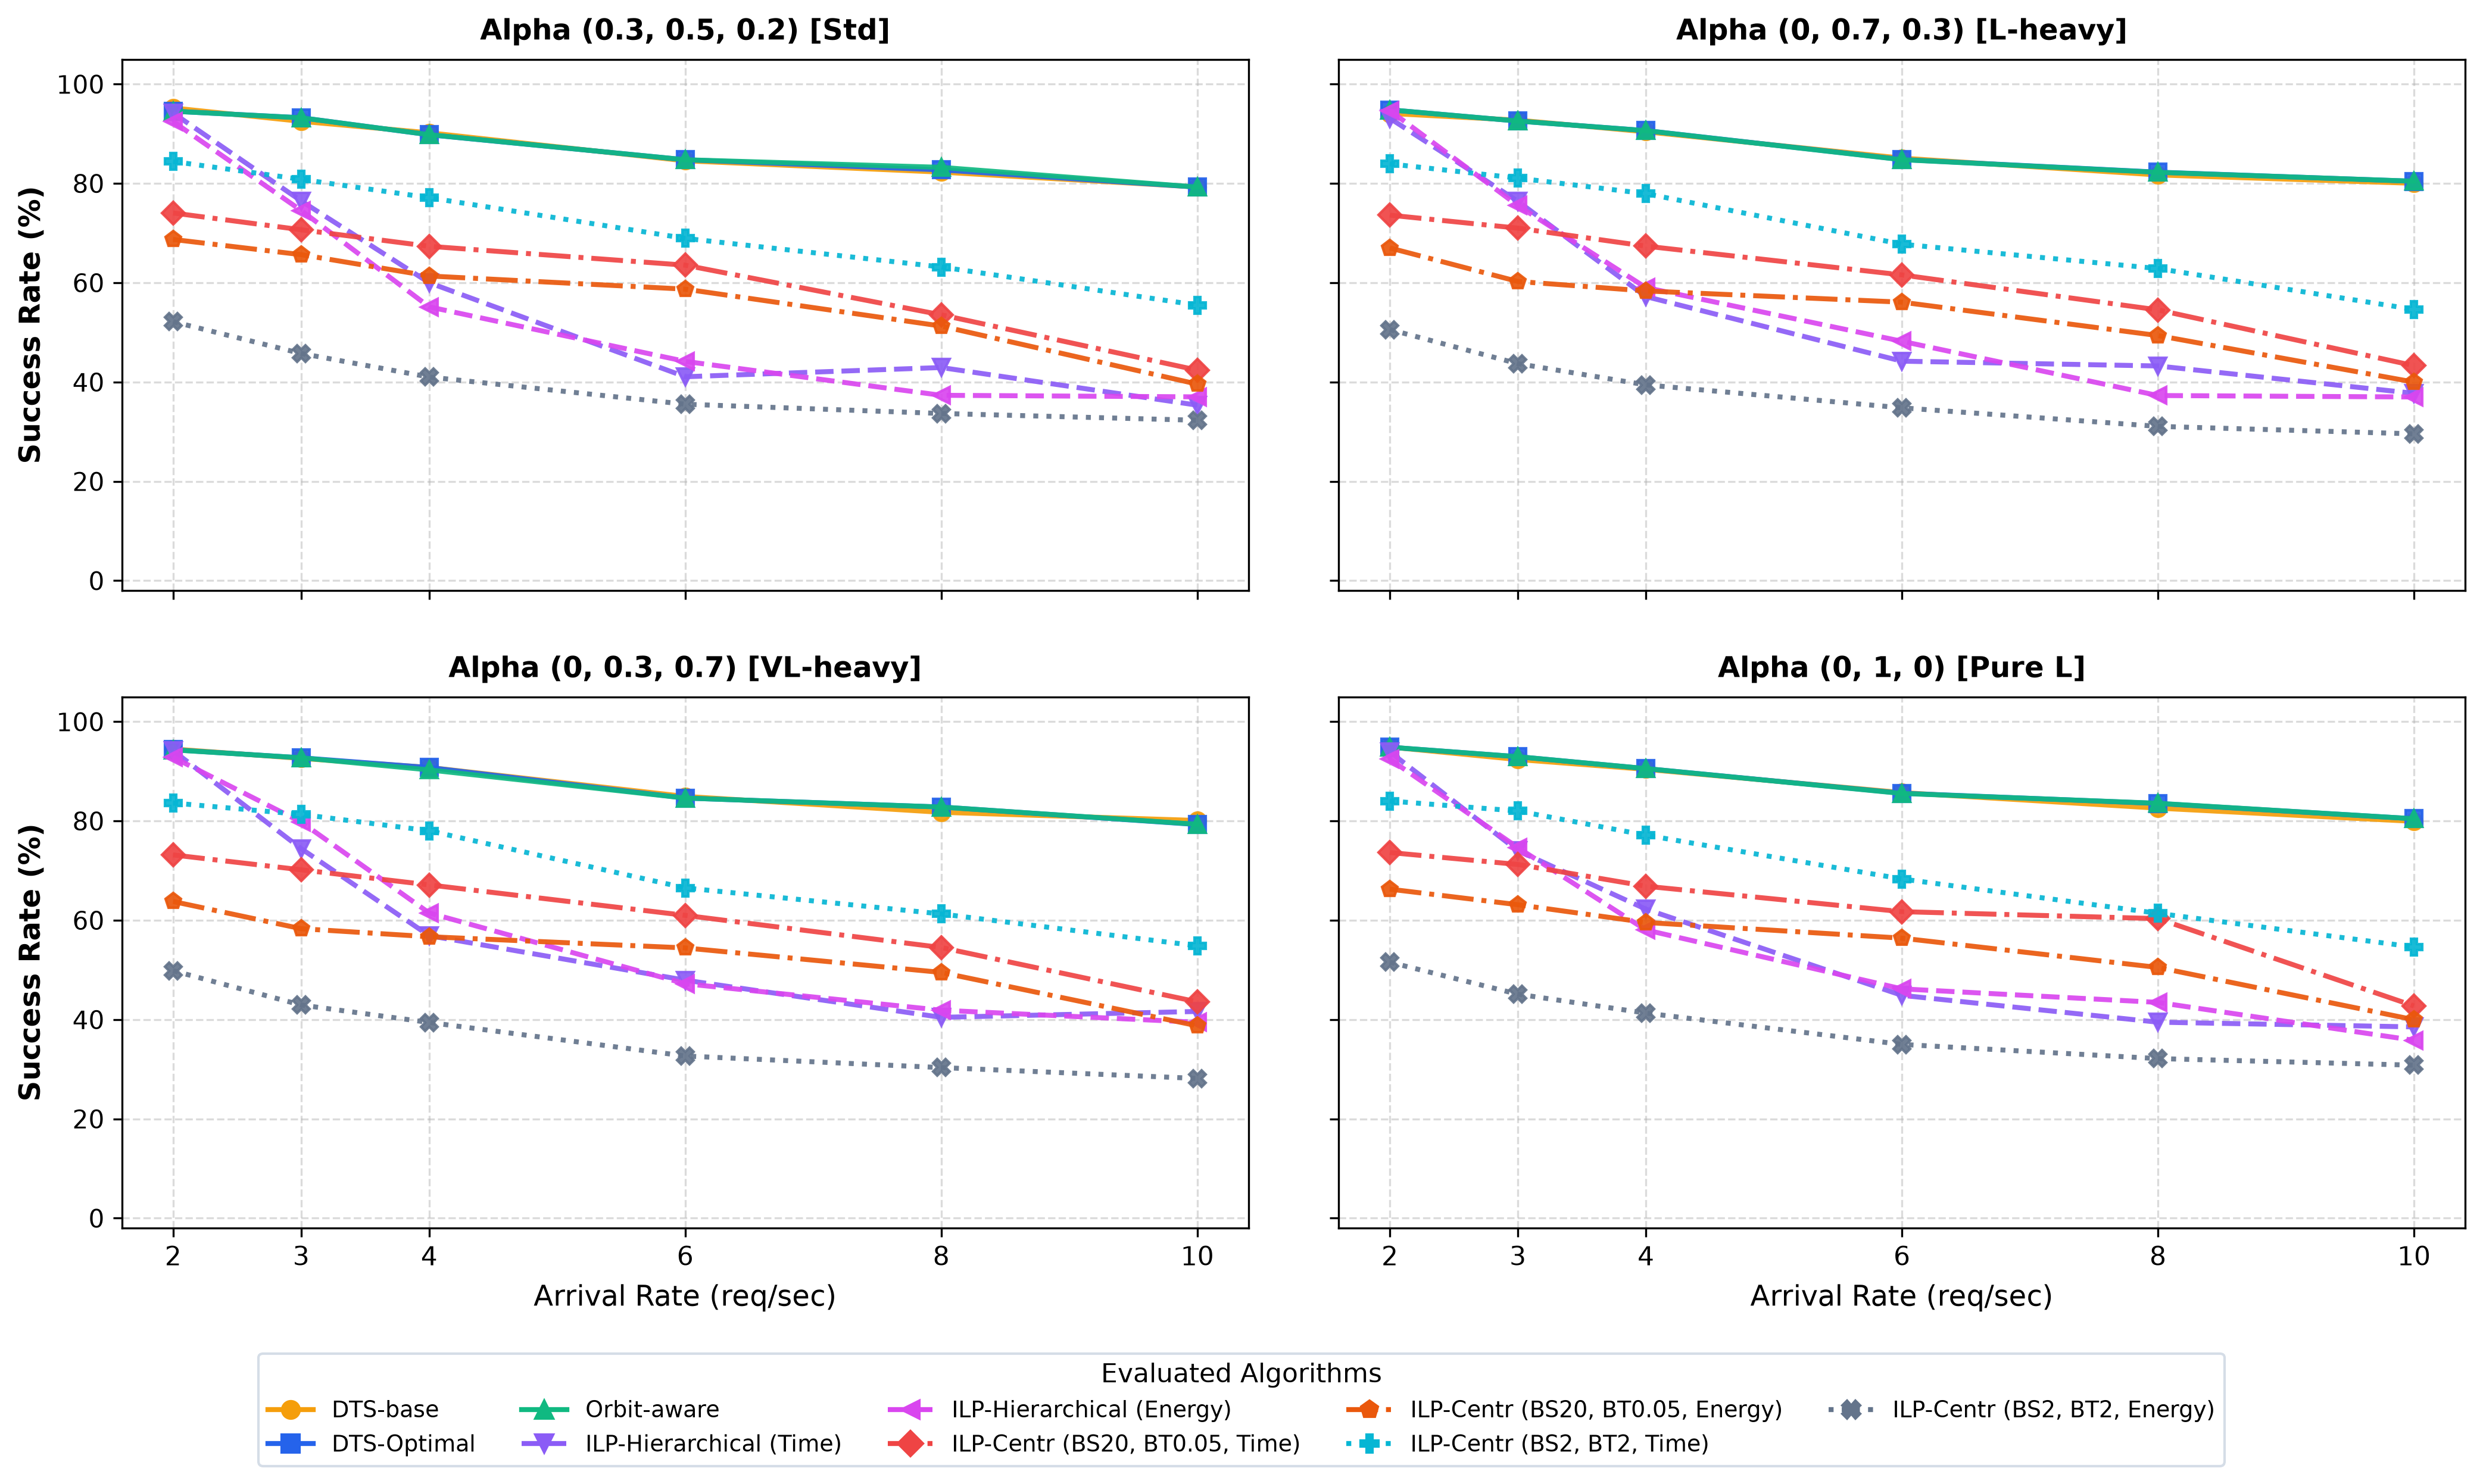
\includegraphics[width=\linewidth]{figures/01_Success_Rate_Beta_0_4_0_35_0_25_40kJ.png} \\
        \vspace{0.3cm}
        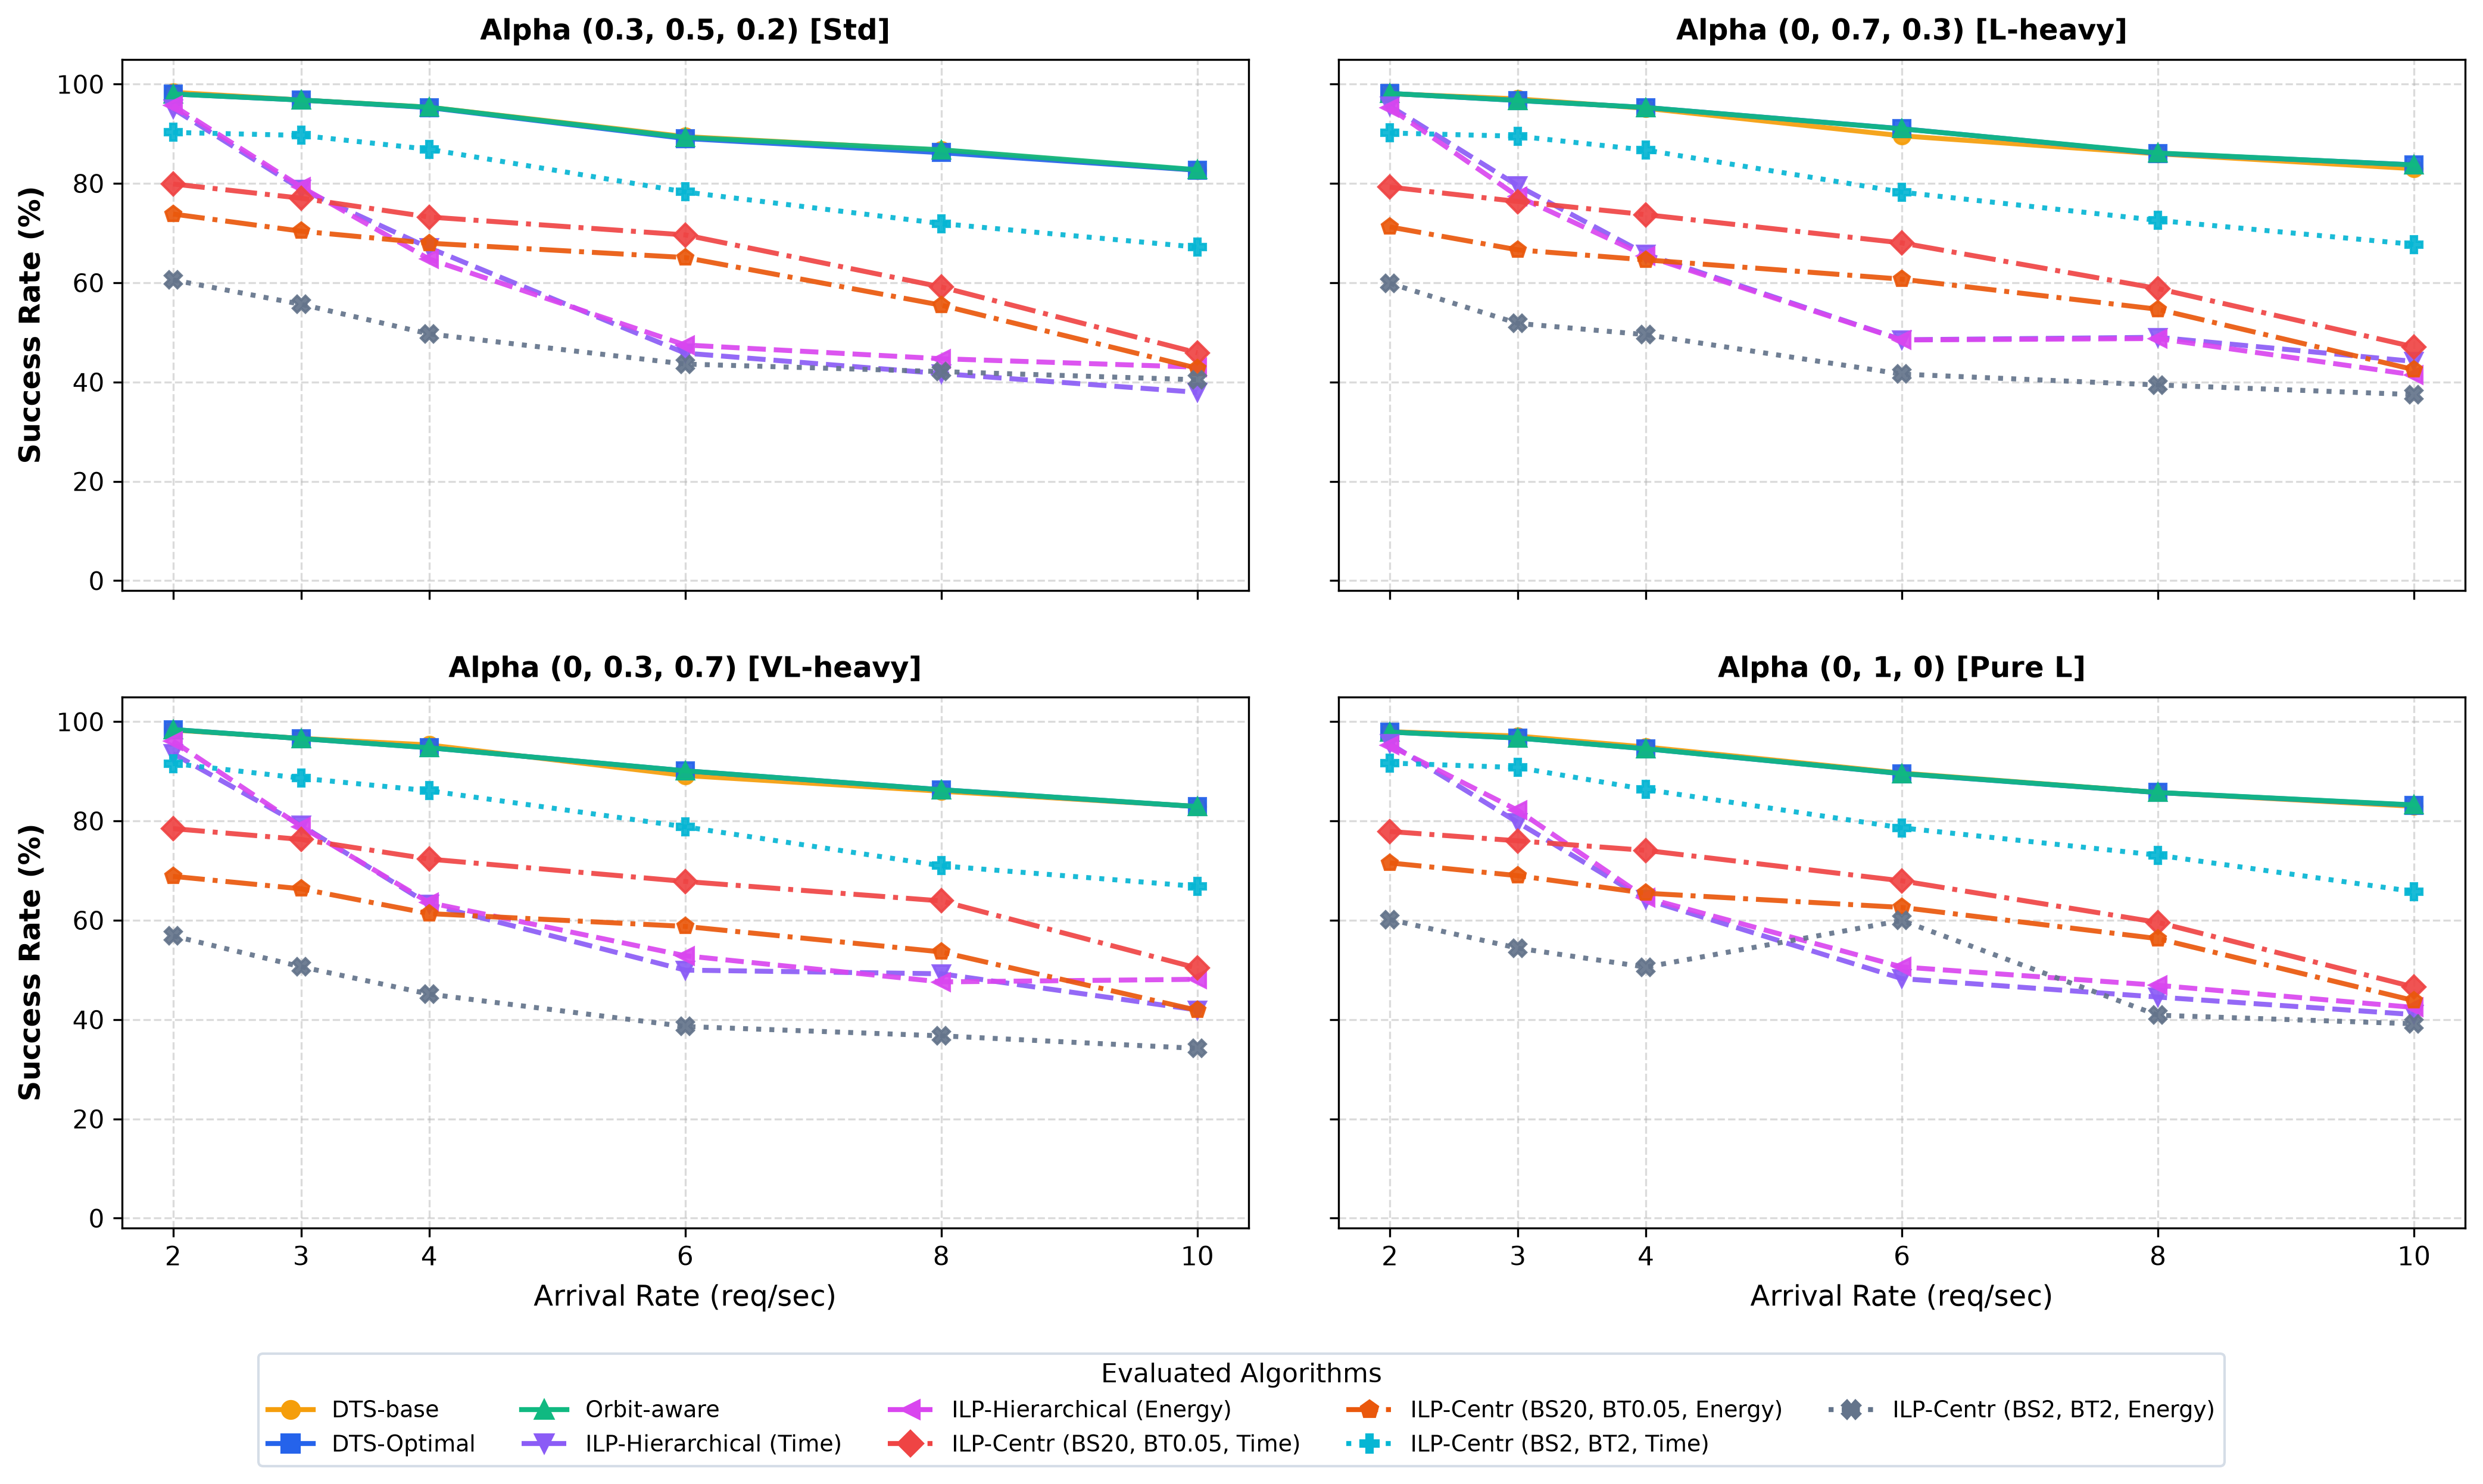
\includegraphics[width=\linewidth]{figures/01_Success_Rate_Beta_0_4_0_35_0_25_80kJ.png}
        \caption{Success Rate across arrival rates under Mixed Workload $\boldsymbol{\beta} = (0.40, 0.35, 0.25)$ for $40\text{ kJ}$ (top) and $80\text{ kJ}$ (bottom) across payload distributions $\boldsymbol{\alpha}$.}
        \label{fig:sr_mixed}
    \end{adjustwidth}
\end{figure}

\begin{figure}[H]
    \begin{adjustwidth}{-1.5cm}{-1.5cm}
        \centering
        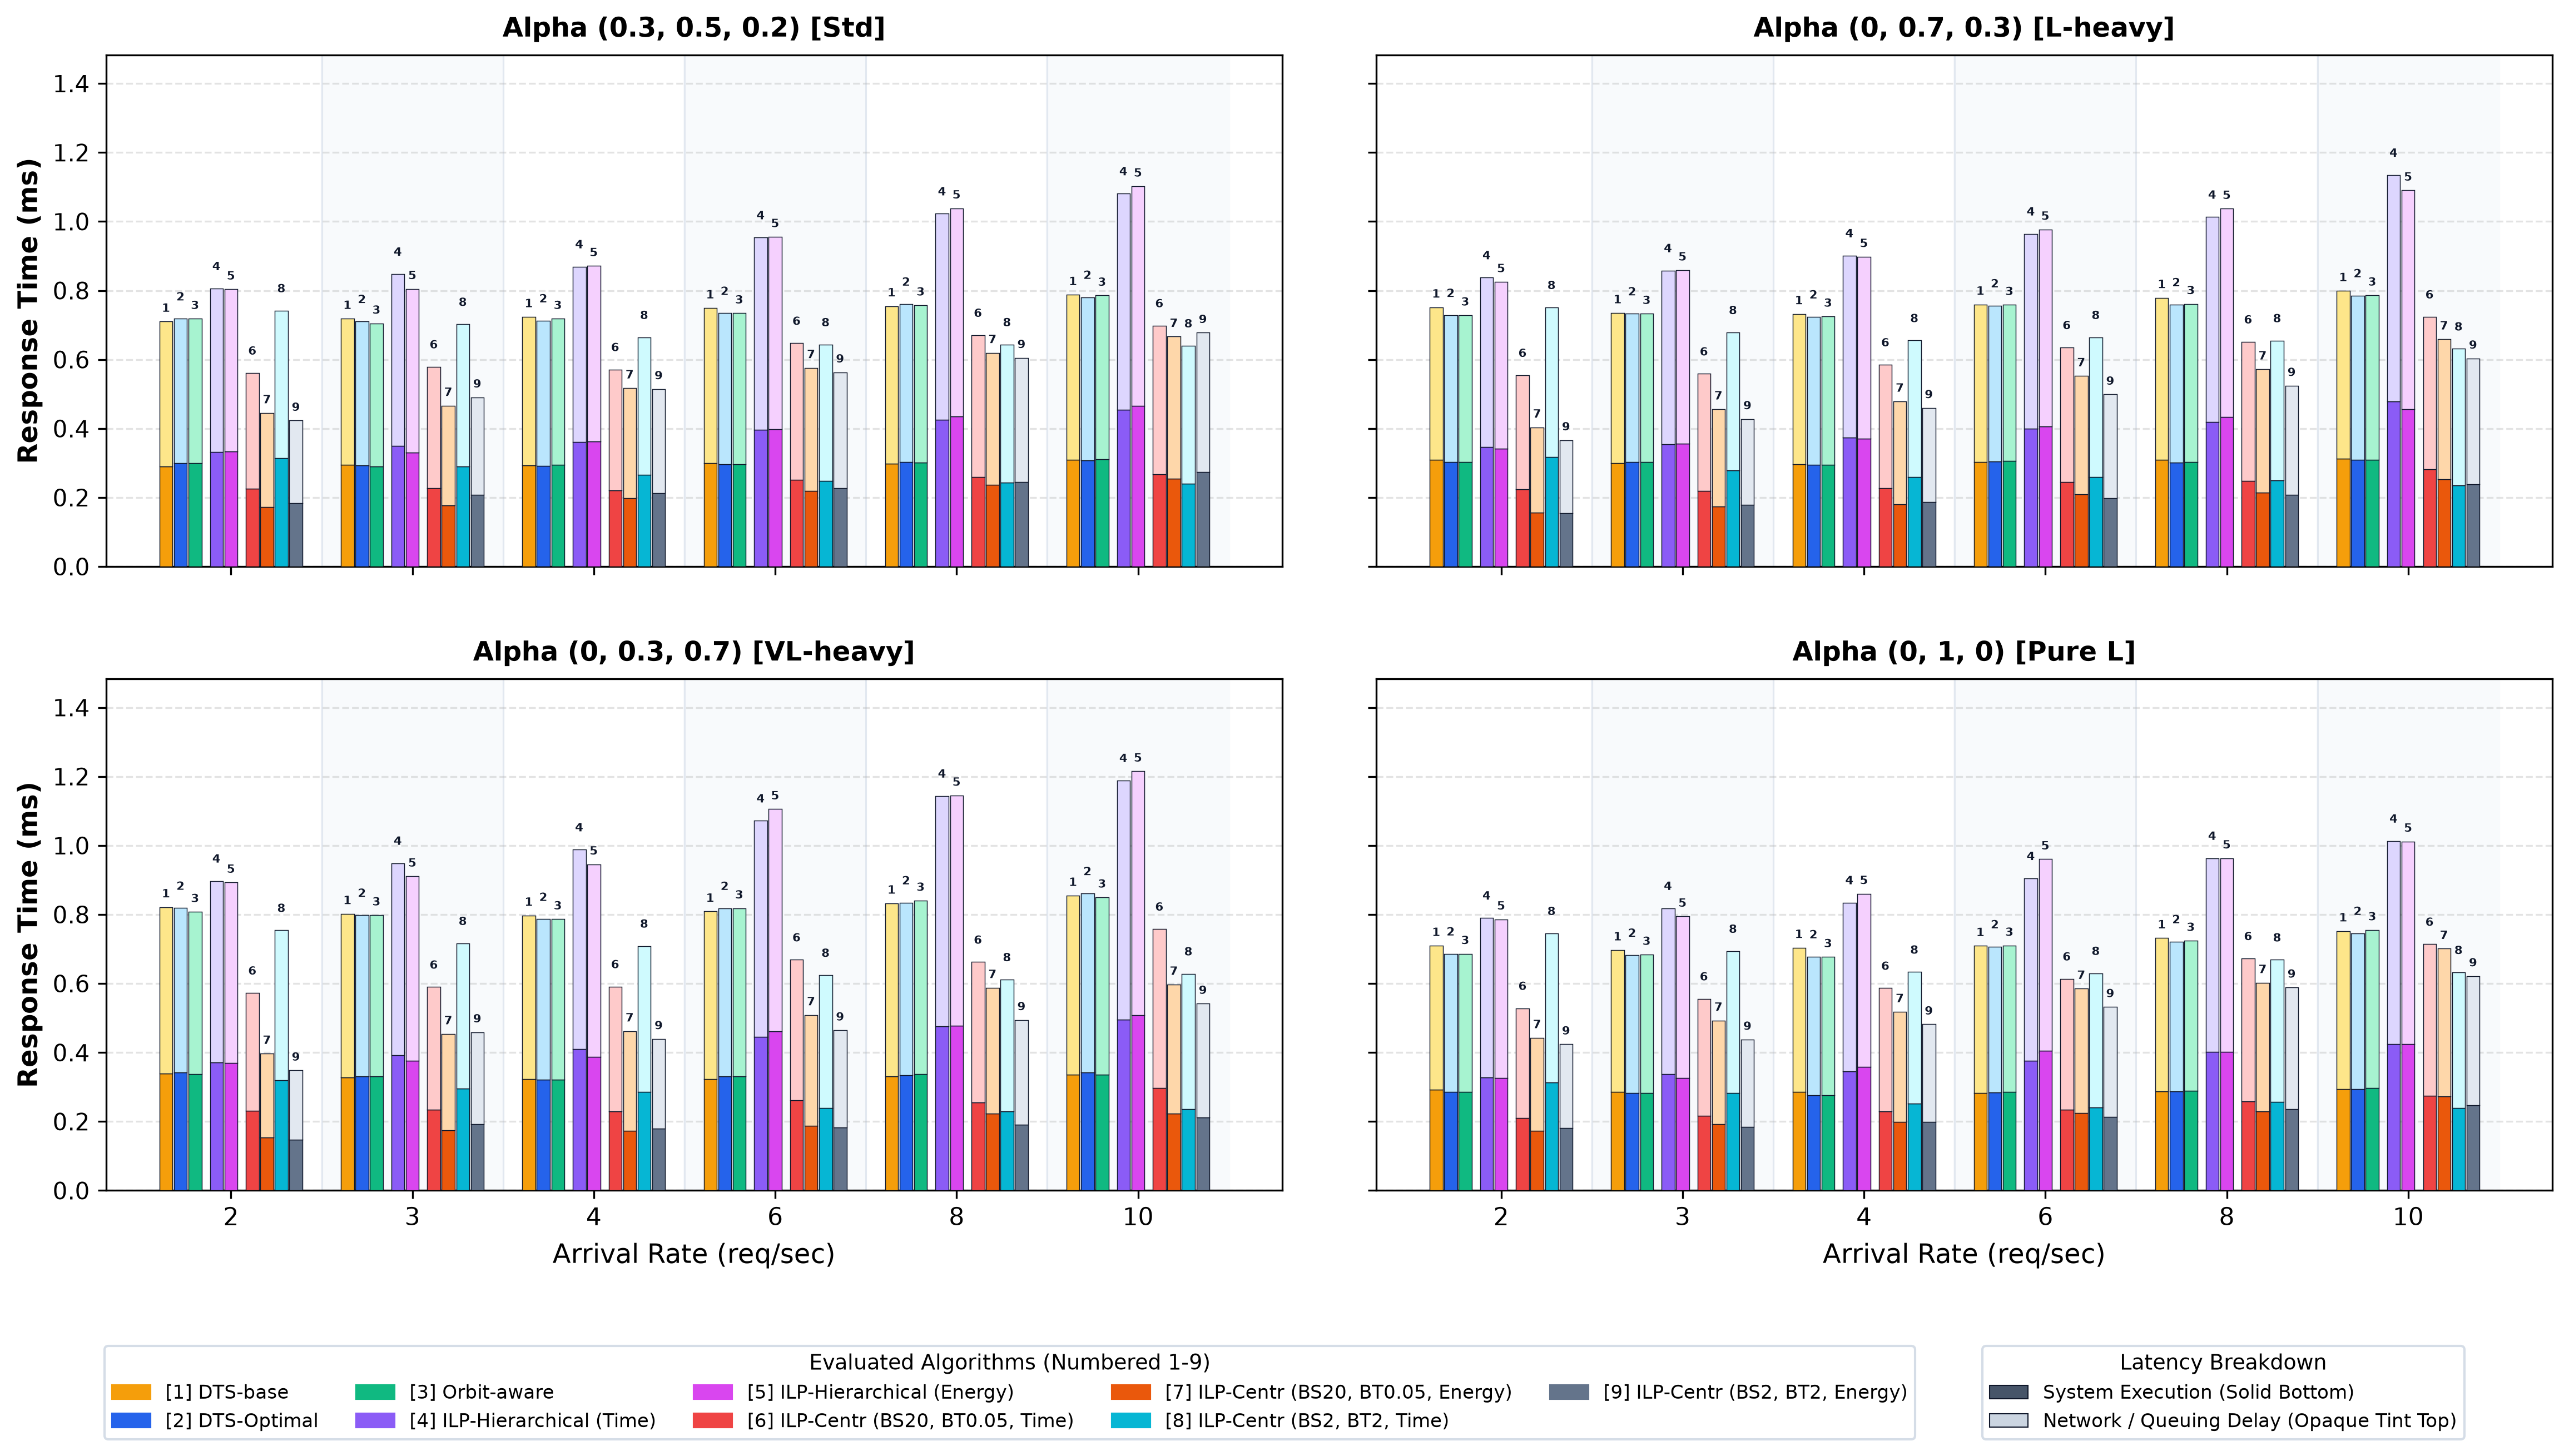
\includegraphics[width=\linewidth]{figures/02_Response_Time_Beta_0_4_0_35_0_25_40kJ.png} \\
        \vspace{0.3cm}
        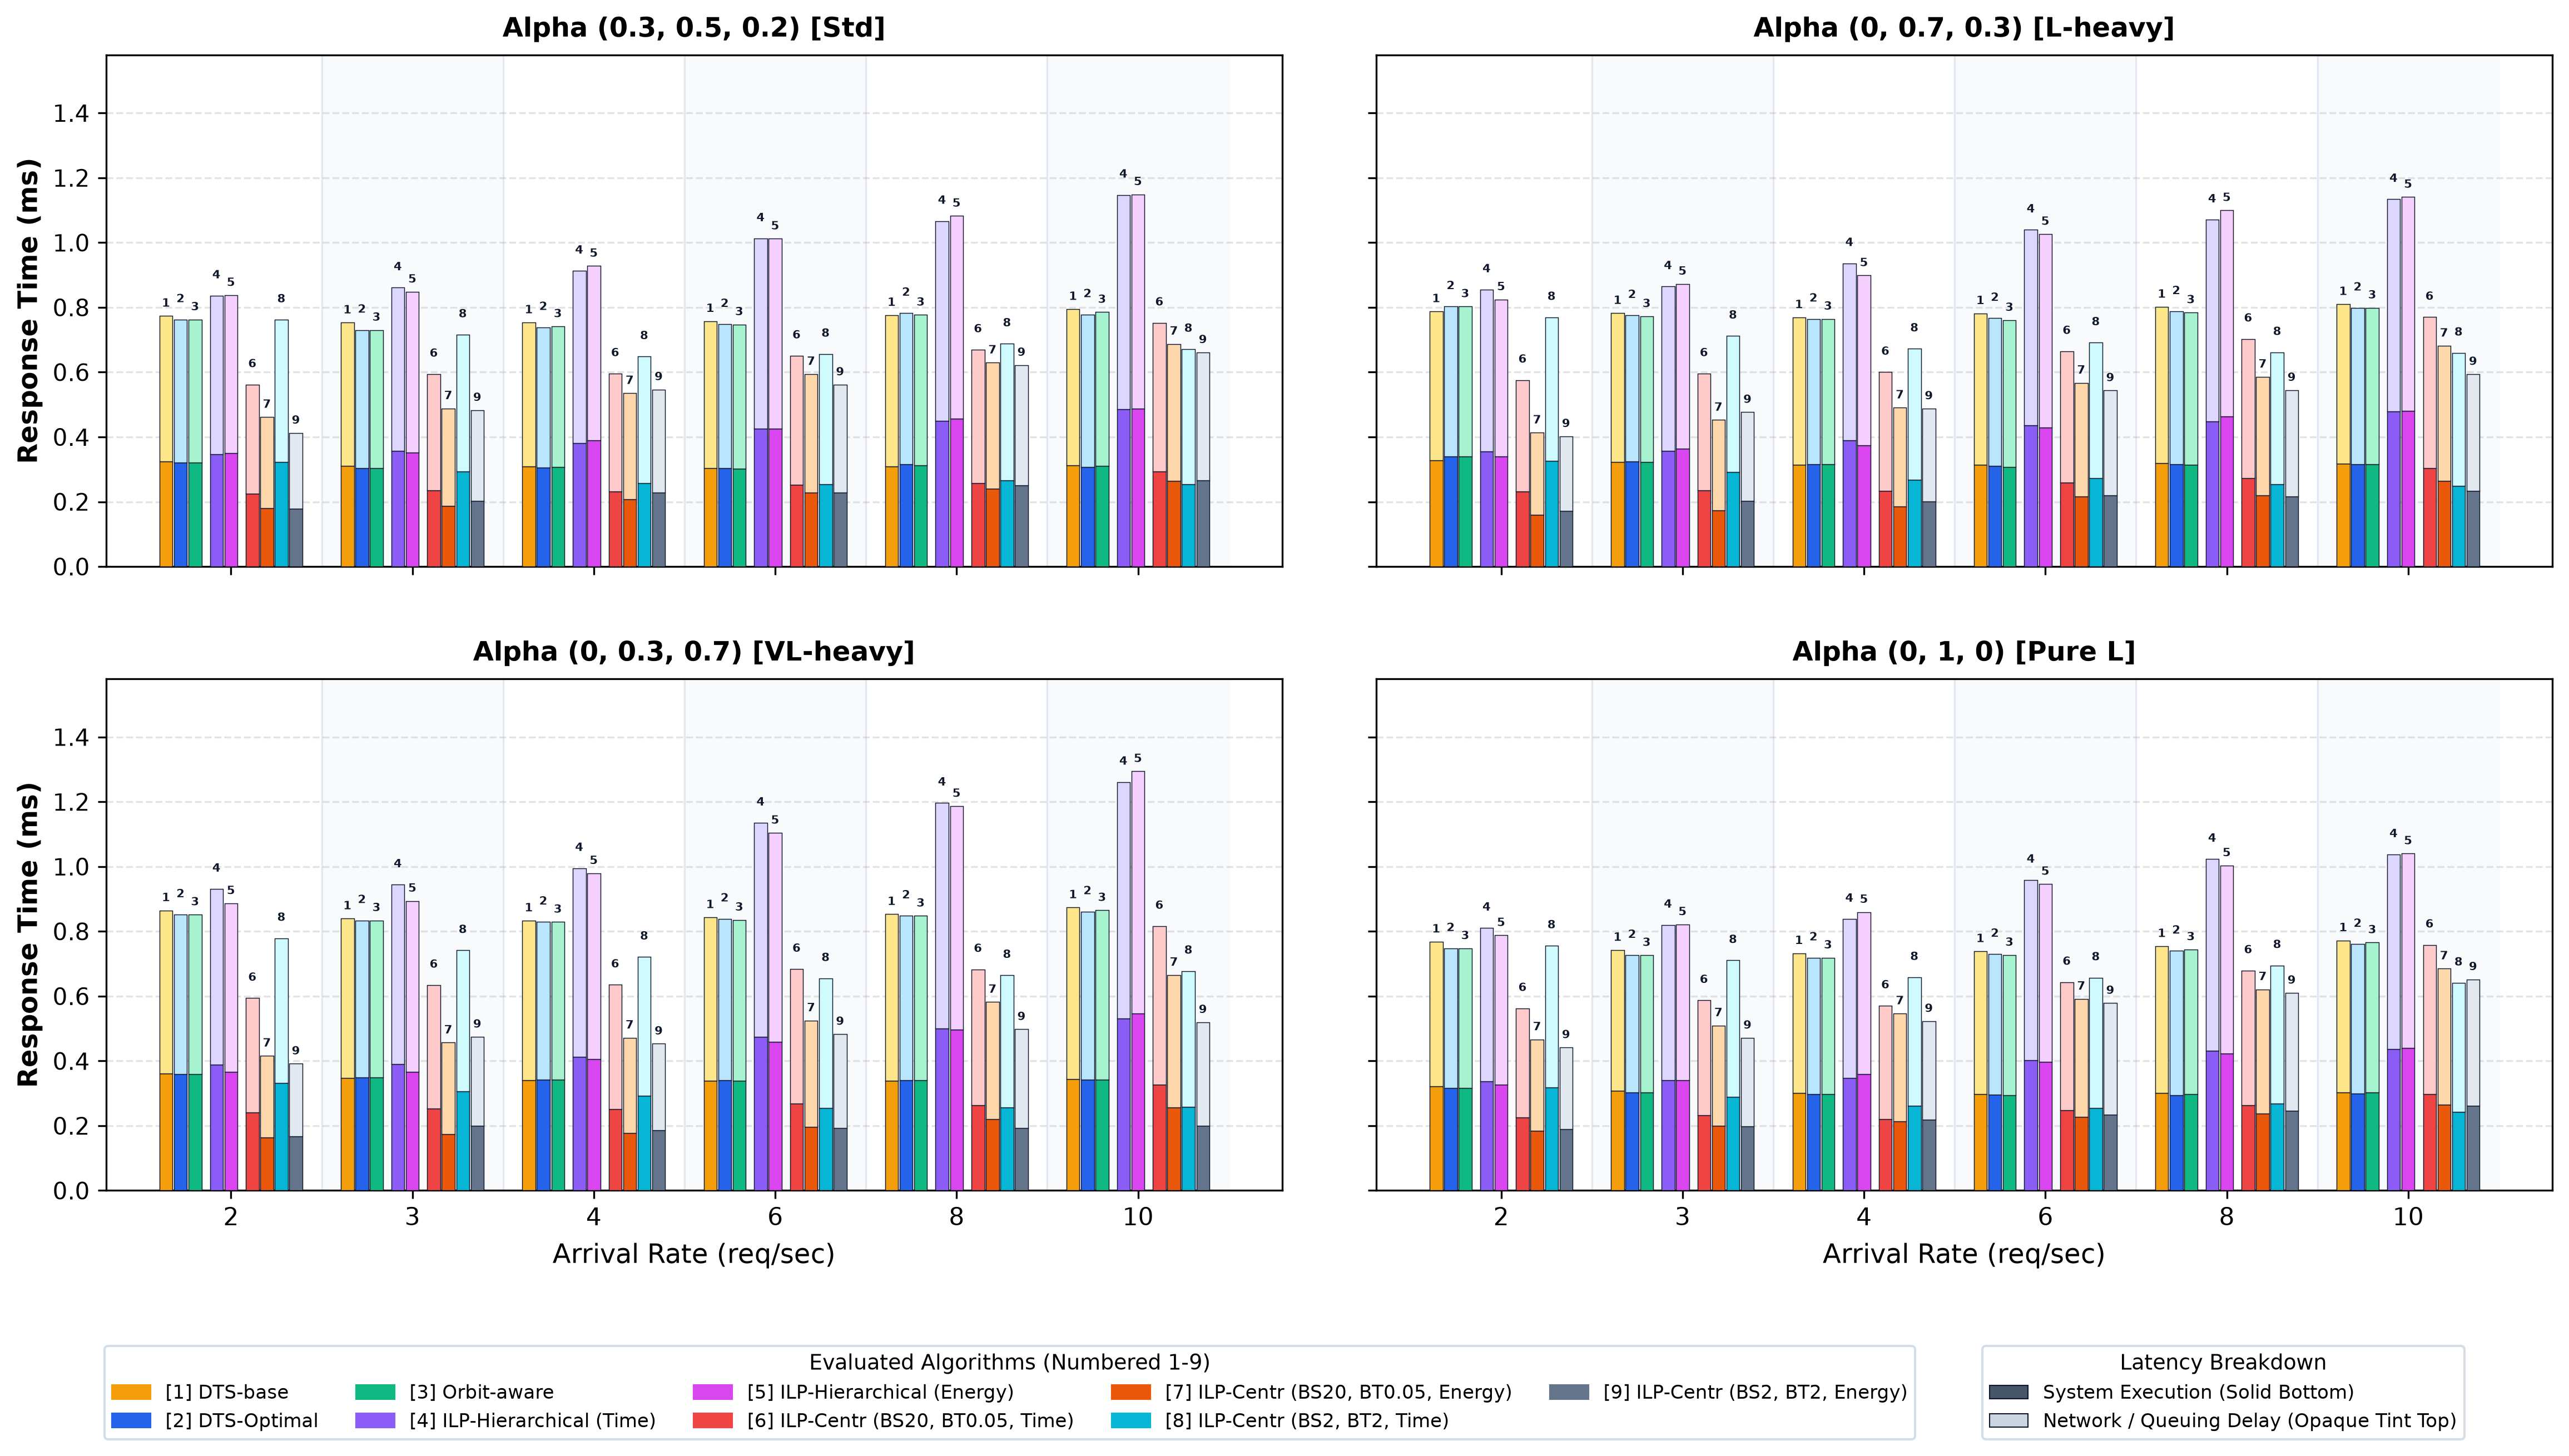
\includegraphics[width=\linewidth]{figures/02_Response_Time_Beta_0_4_0_35_0_25_80kJ.png}
        \caption{Response Time decomposition under Mixed Workload $\boldsymbol{\beta} = (0.40, 0.35, 0.25)$ comparing Onboard Task Execution and Network/Wait latency for $40\text{ kJ}$ (top) and $80\text{ kJ}$ (bottom).}
        \label{fig:rt_mixed}
    \end{adjustwidth}
\end{figure}

\begin{figure}[H]
    \begin{adjustwidth}{-1.5cm}{-1.5cm}
        \centering
        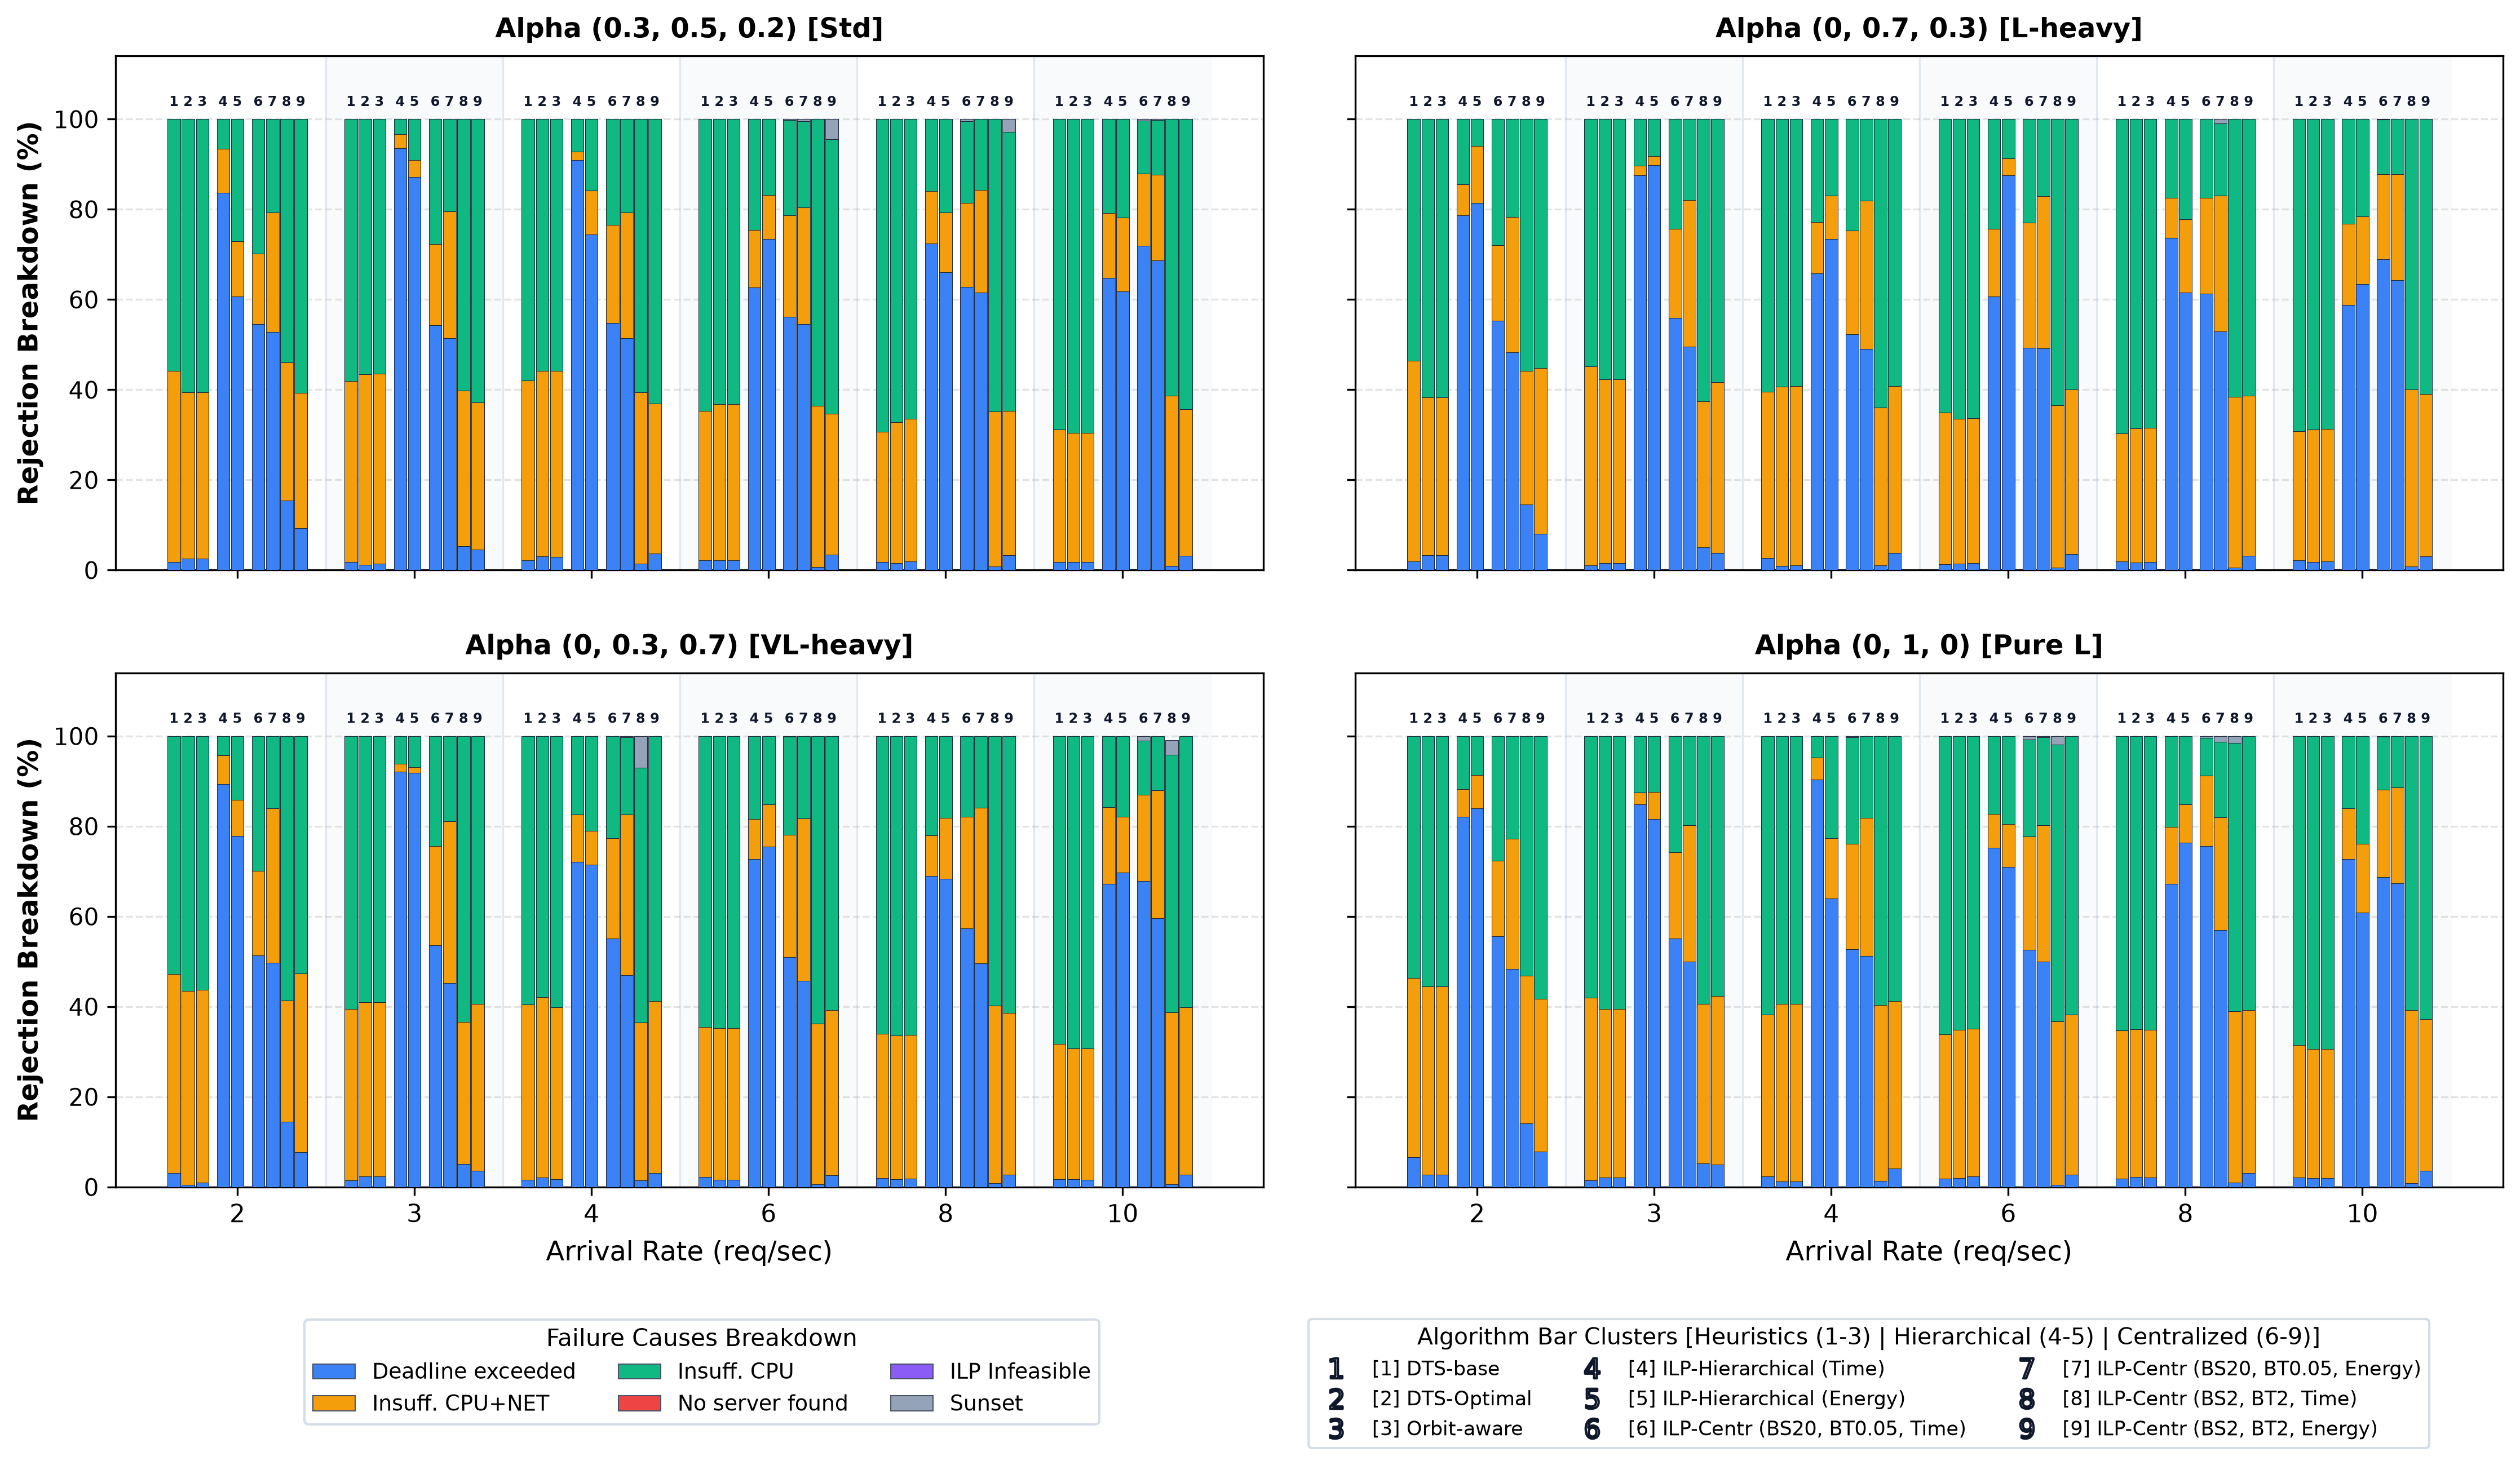
\includegraphics[width=\linewidth]{figures/03_Rejection_Causes_Beta_0_4_0_35_0_25_40kJ.png} \\
        \vspace{0.3cm}
        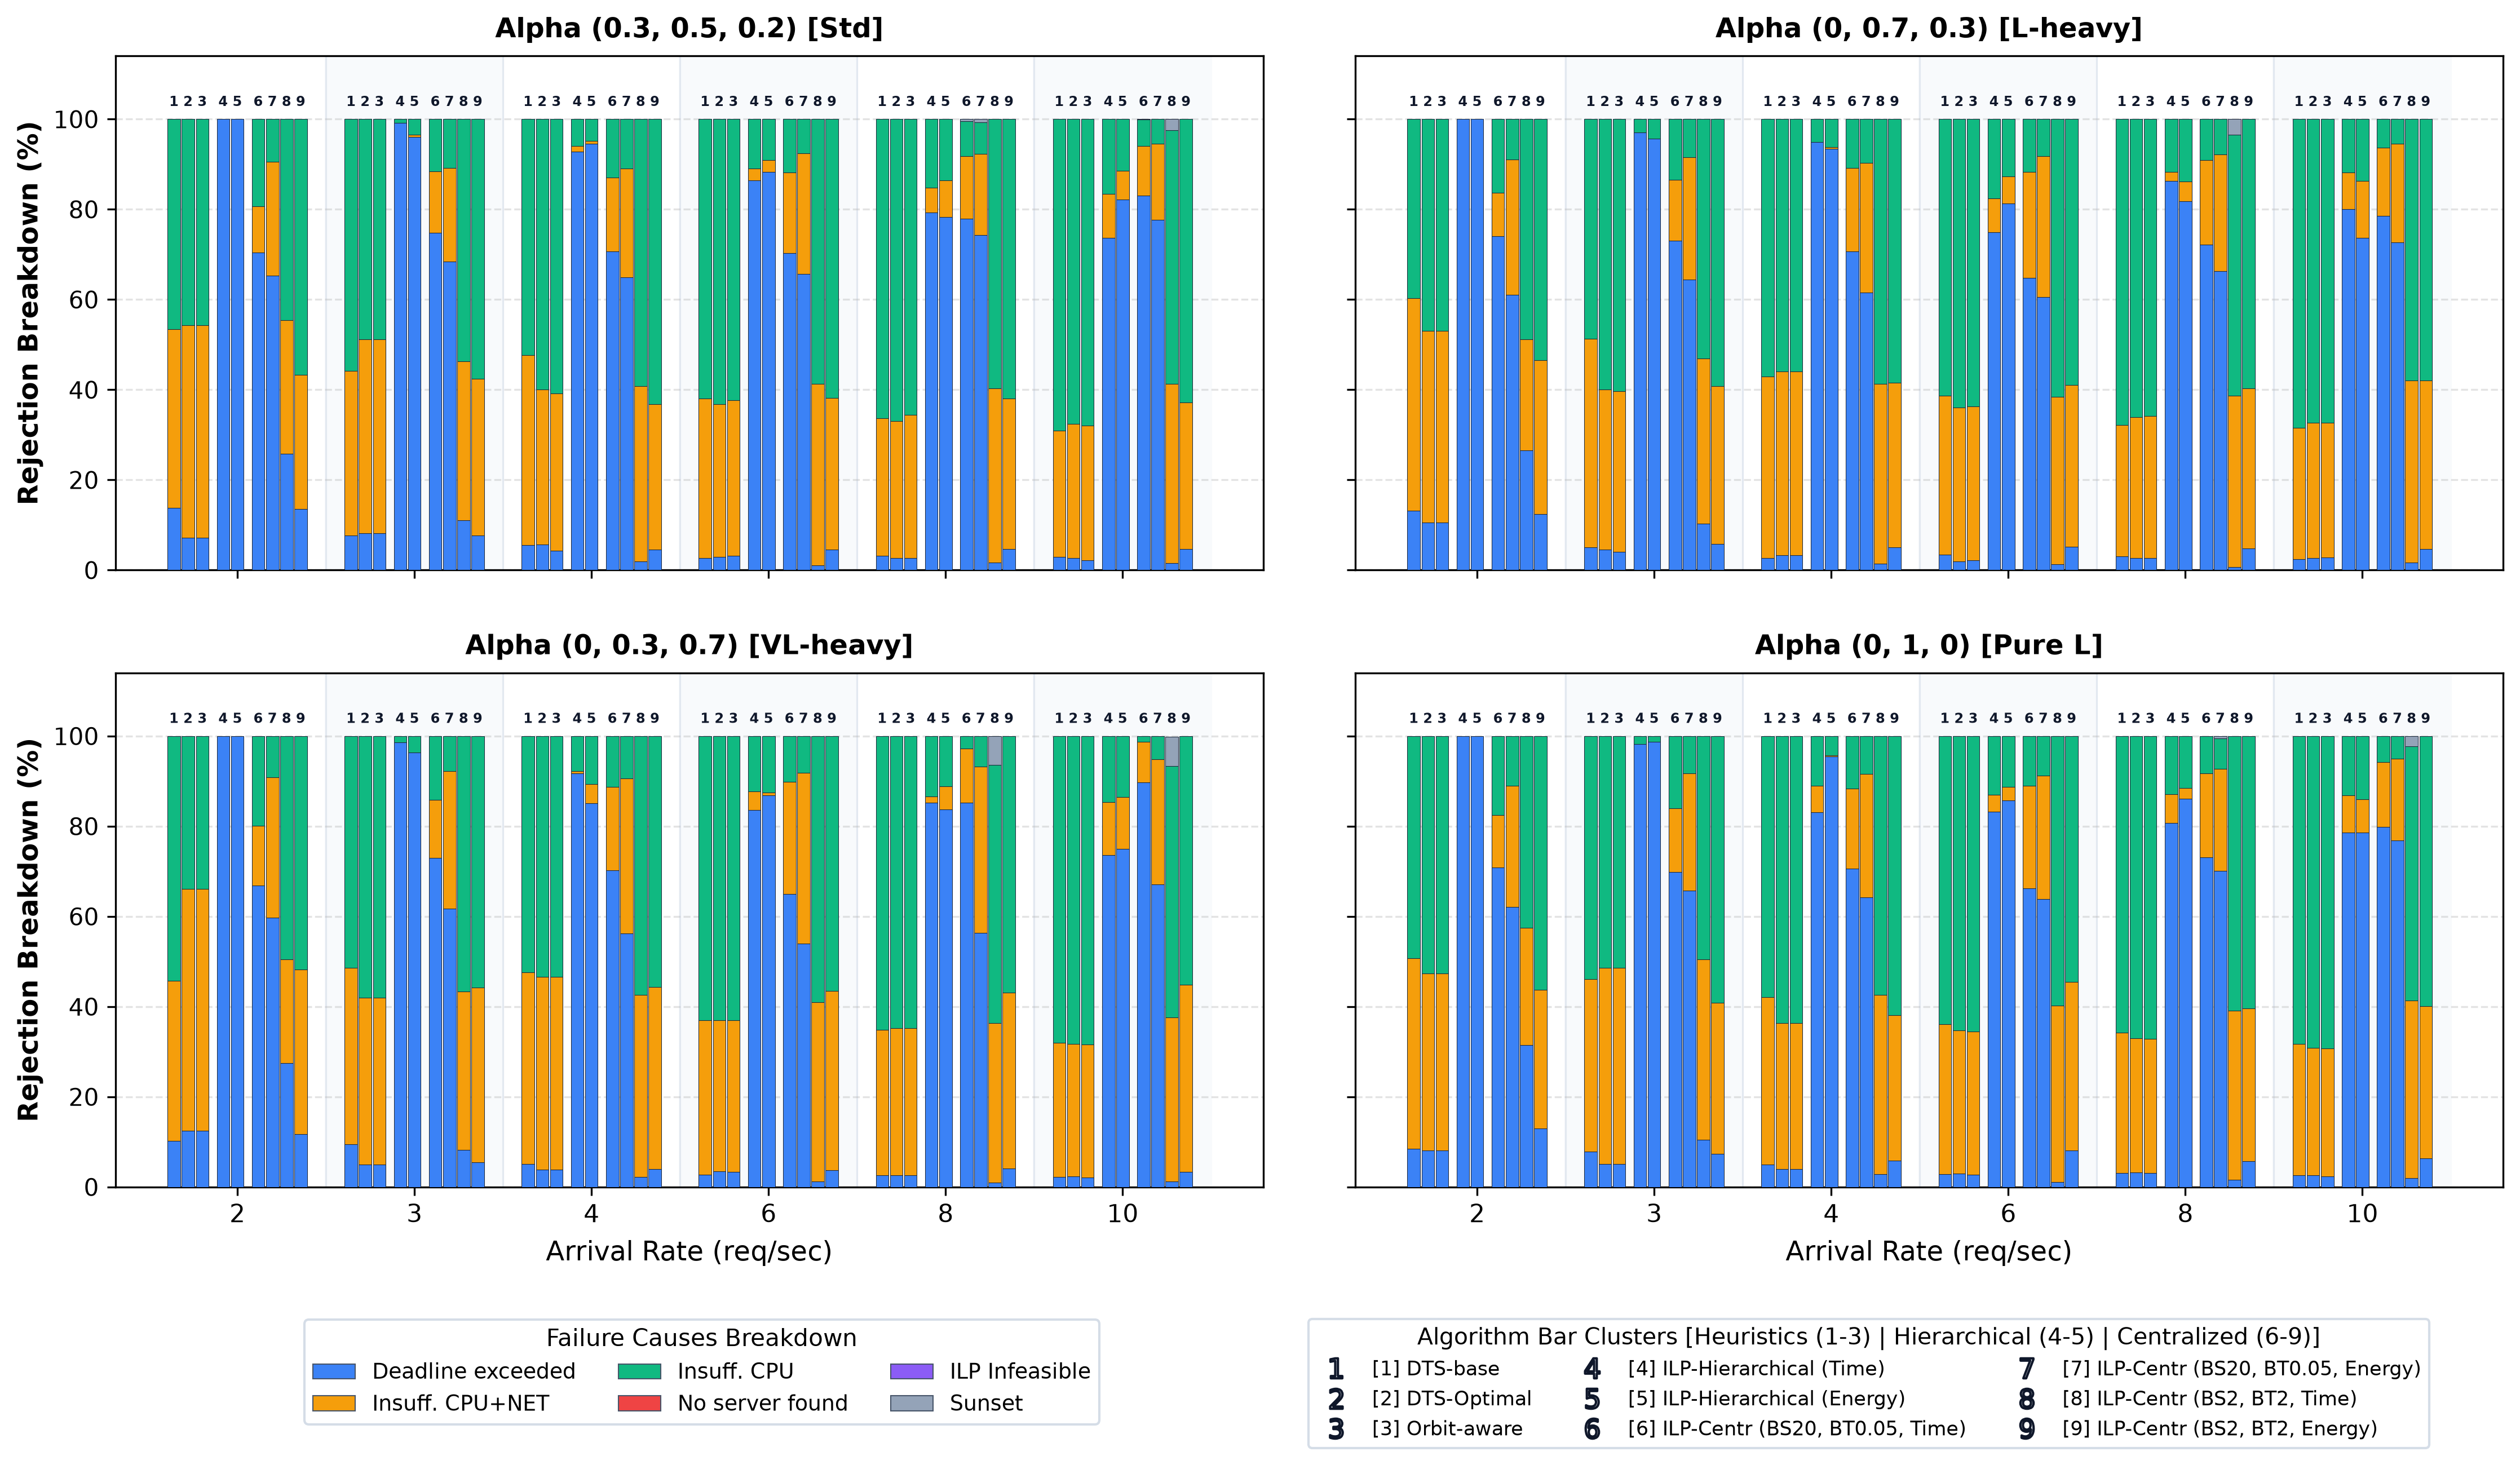
\includegraphics[width=\linewidth]{figures/03_Rejection_Causes_Beta_0_4_0_35_0_25_80kJ.png}
        \caption{Rejection Causes distribution under Mixed Workload $\boldsymbol{\beta} = (0.40, 0.35, 0.25)$ across arrival rates for $40\text{ kJ}$ (top) and $80\text{ kJ}$ (bottom).}
        \label{fig:rej_mixed}
    \end{adjustwidth}
\end{figure}

\subsubsection{Success Rate Dynamics}
Under low arrival rates ($\lambda = 2\text{ req/s}$), all distributed heuristics achieve exceptional completion rates exceeding $90\%$. The centralized orchestrator with fast-dispatch (\texttt{ILP-Centr [BS20, BT0.05]}) demonstrates competitive throughput, reaching $\approx 74\%$, while the small-batching configuration (\texttt{ILP-Centr [BS2, BT2]}) achieves slightly higher initial rates. As traffic scales to $\lambda = 10\text{ req/s}$, heuristics maintain superiority ($\approx 80\%$), while optimization models experience degradation due to queuing delays. The subplots reveal that shifting the payload distribution to \textit{VL-heavy} or \textit{Pure L} exacerbates success rate decay, placing further strain on optical link capacities.

\subsubsection{Response Time Analysis}
Figure~\ref{fig:rt_mixed} highlights a structural divergence in latency components. Distributed heuristics achieve flat response times across all arrival rates ($\approx 0.70\text{ ms}$) because their localized decision-making incurs zero ingress queuing delay. In contrast, optimization models display latency expansion under heavy load, driven entirely by $T_{net+wait}$ (the opaque upper bar). Crucially, the physical execution time on the destination SEN CPU cores ($T_{exec}$, the solid bottom bar) remains highly stable and invariant ($\le 0.30\text{ ms}$) across all configurations. This confirms that the physical processing of tasks on space-qualified hardware does not bottleneck the system; latency growth is strictly an artifact of batch waiting times.

\subsubsection{Failure Diagnostics}
Figure~\ref{fig:rej_mixed} details the diagnostic failure profile. Because the workload is mixed, rejections for distributed heuristics are split between physical bottlenecks: \textit{Insufficient CPU} (green) and \textit{Insufficient CPU+NET} (orange). For ILP-based models, \textit{Deadline Exceeded} (blue) emerges as a substantial failure cause ($\approx 40\text{--}60\%$ of drops), confirming that optimization models fail primarily because ingress waiting time erodes the slack time before local execution on the SEN can even commence.

% -----------------------------------------------------------------------------
% SUBSECTION 5.2.2: CPU-INTENSIVE WORKLOAD
% -----------------------------------------------------------------------------
\subsection{Computation-Heavy Stress: CPU-Intensive Profile (\texorpdfstring{$\boldsymbol{\beta} = (0, 1, 0)$}{beta = (0, 1, 0)})}
\label{subsec:bench_cpu}

When the workload consists entirely of compute-intensive requests with minimal payload transfer ($\boldsymbol{\beta} = (0, 1, 0)$), onboard processor clock cycles become the primary system bottleneck.

\begin{figure}[H]
    \begin{adjustwidth}{-1.5cm}{-1.5cm}
        \centering
        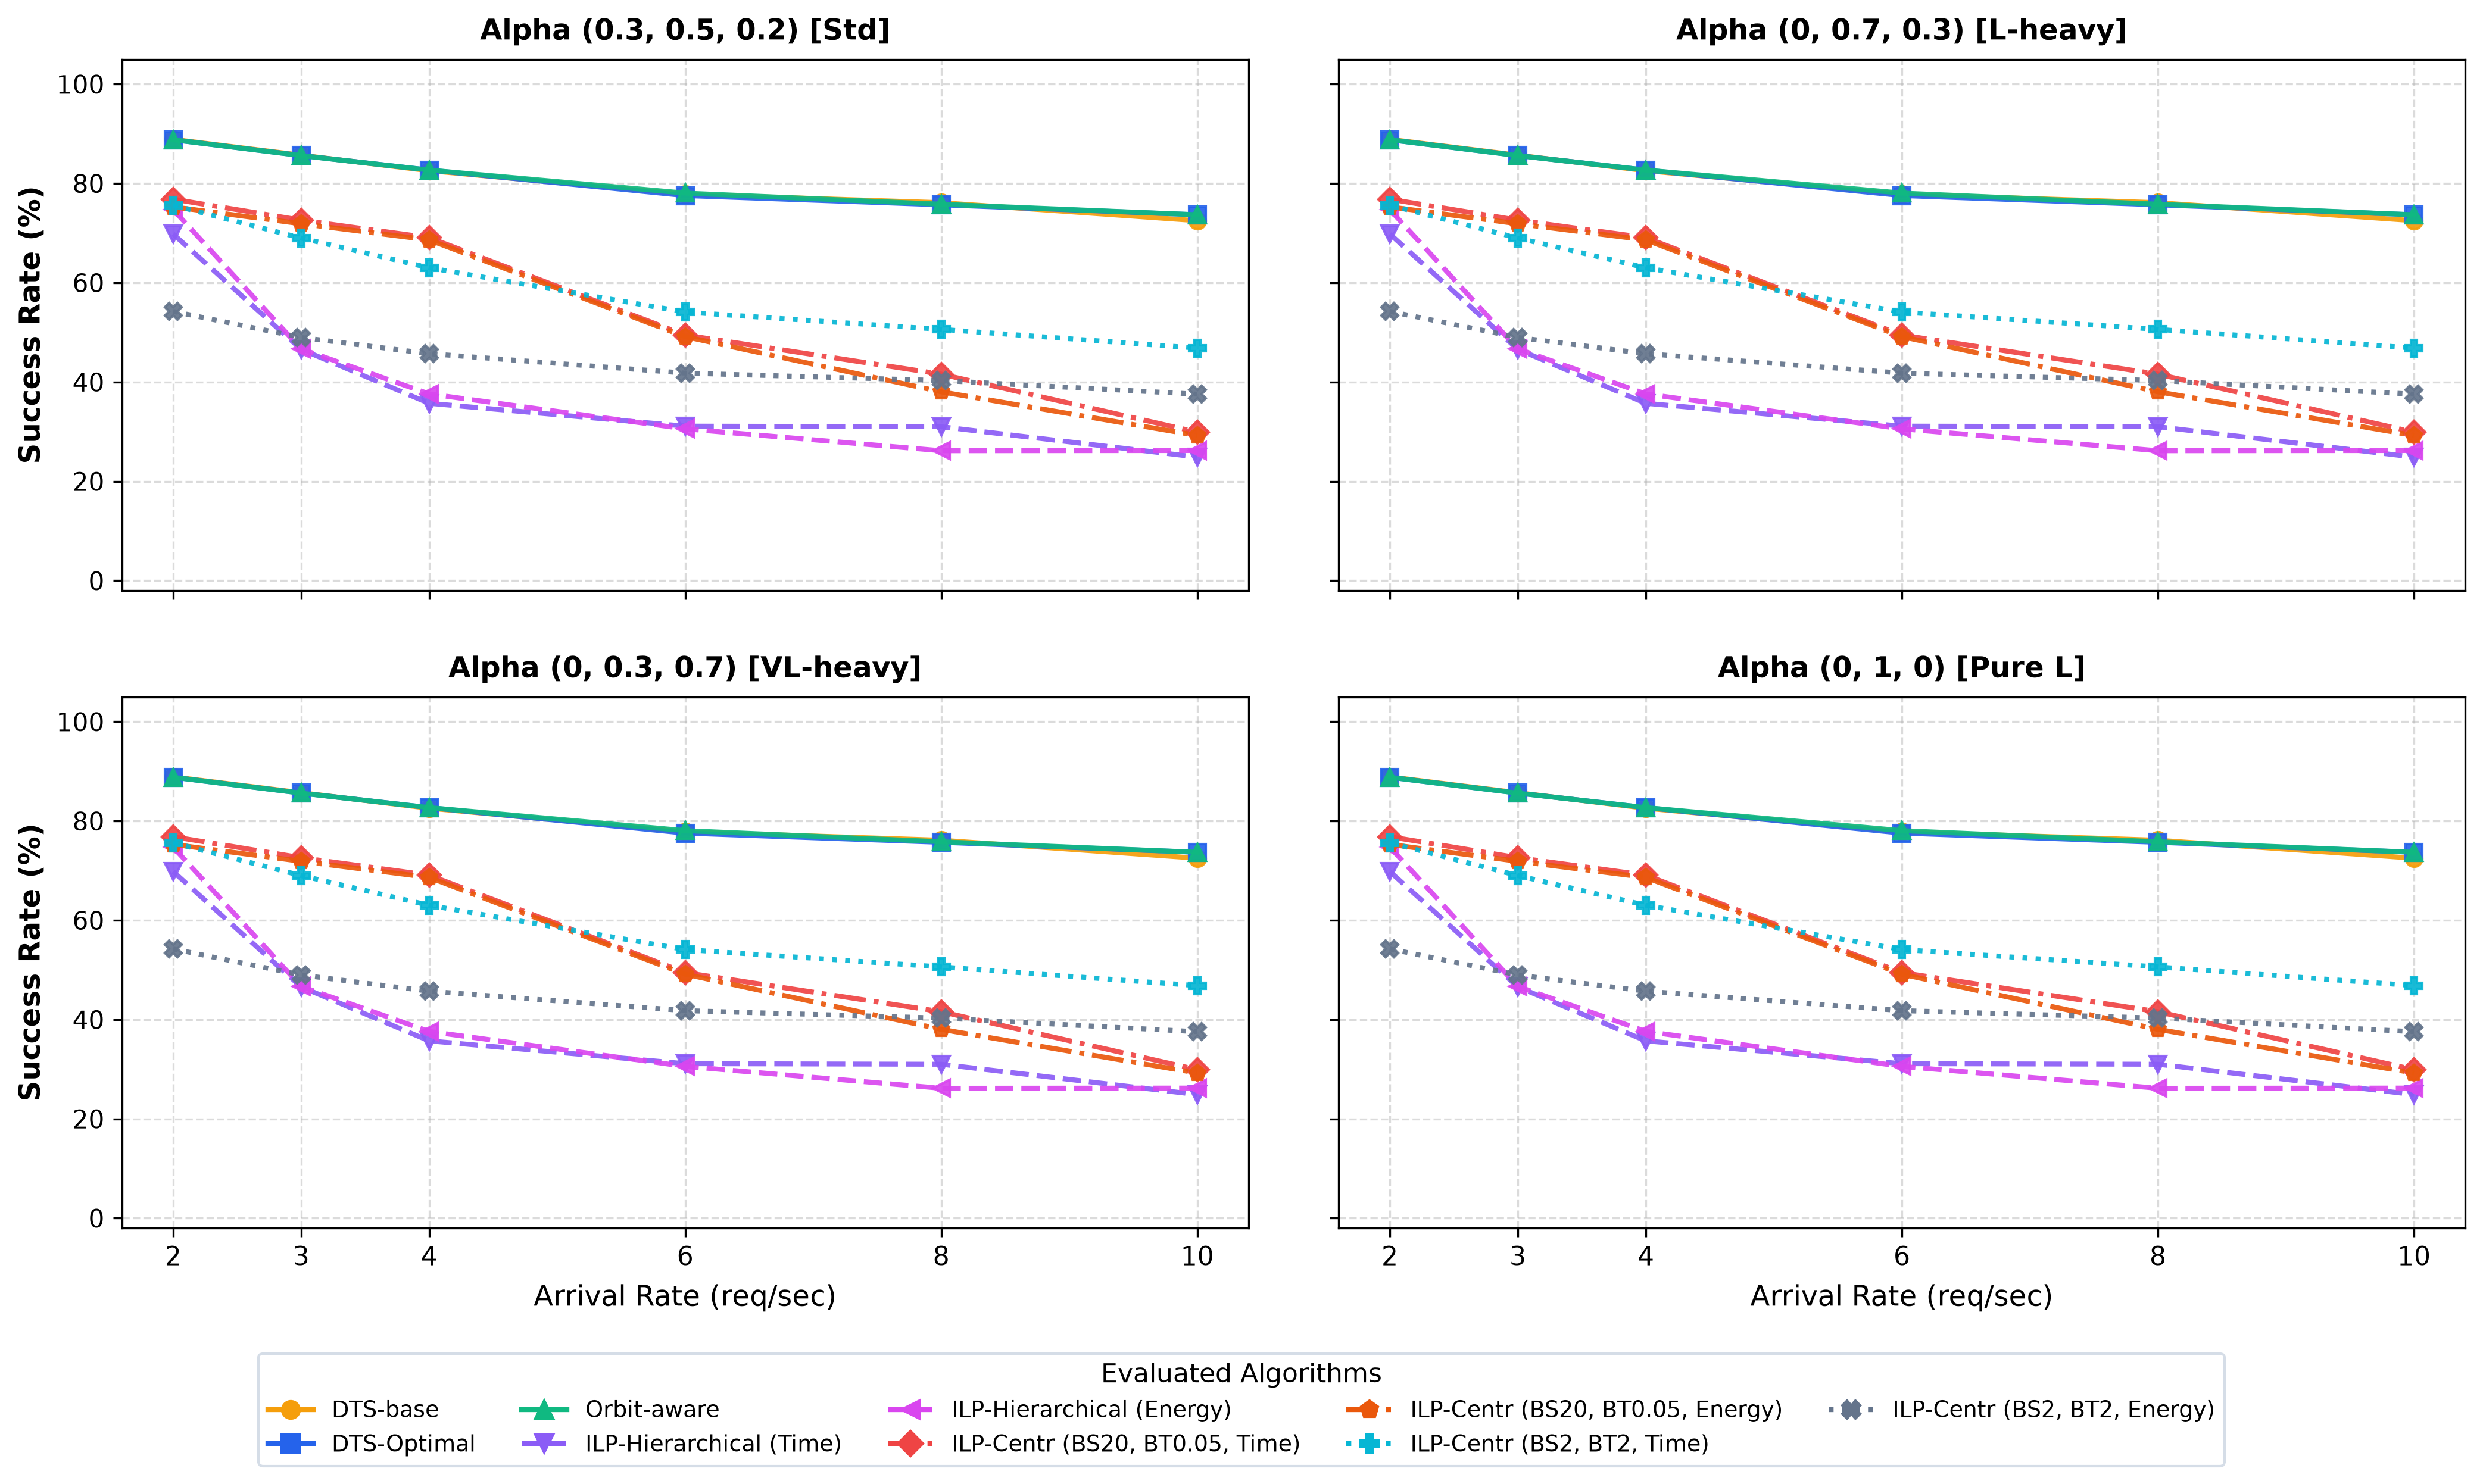
\includegraphics[width=\linewidth]{figures/01_Success_Rate_Beta_0_1_0_40kJ.png} \\
        \vspace{0.3cm}
        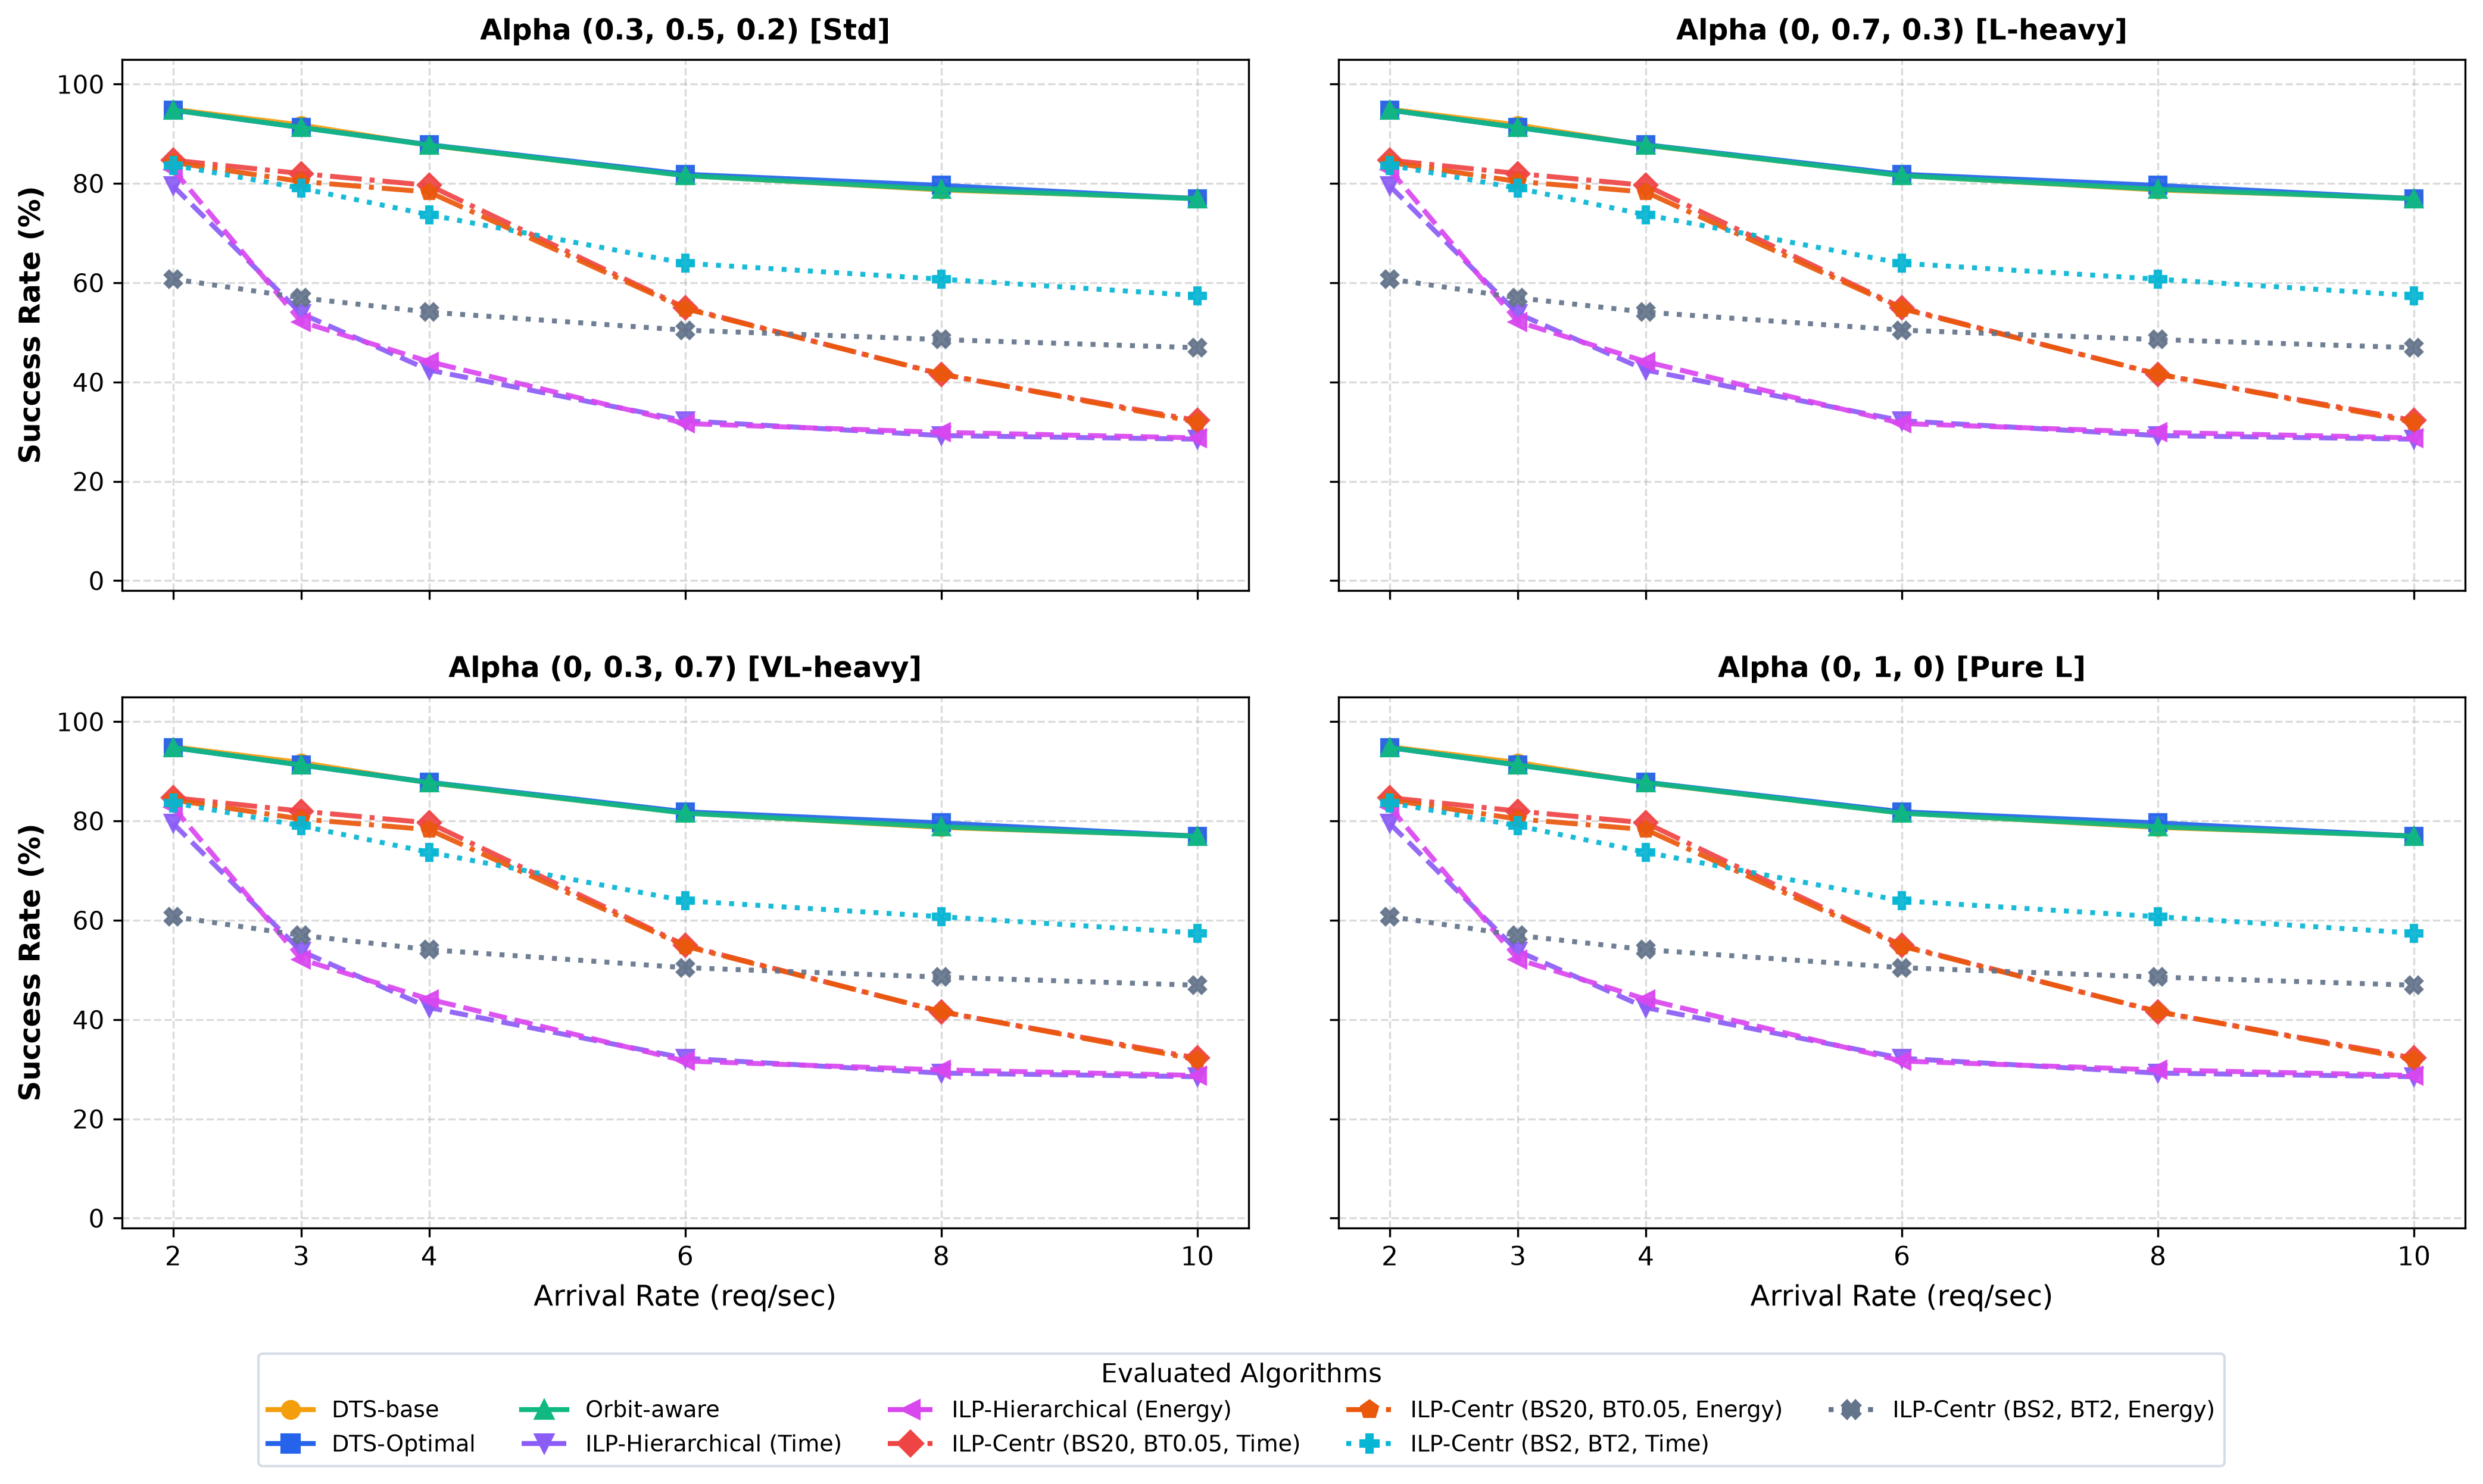
\includegraphics[width=\linewidth]{figures/01_Success_Rate_Beta_0_1_0_80kJ.png}
        \caption{Success Rate across arrival rates under CPU-Intensive Workload $\boldsymbol{\beta} = (0, 1, 0)$ for $40\text{ kJ}$ (top) and $80\text{ kJ}$ (bottom) across payload distributions $\boldsymbol{\alpha}$.}
        \label{fig:sr_cpu}
    \end{adjustwidth}
\end{figure}

\begin{figure}[H]
    \begin{adjustwidth}{-1.5cm}{-1.5cm}
        \centering
        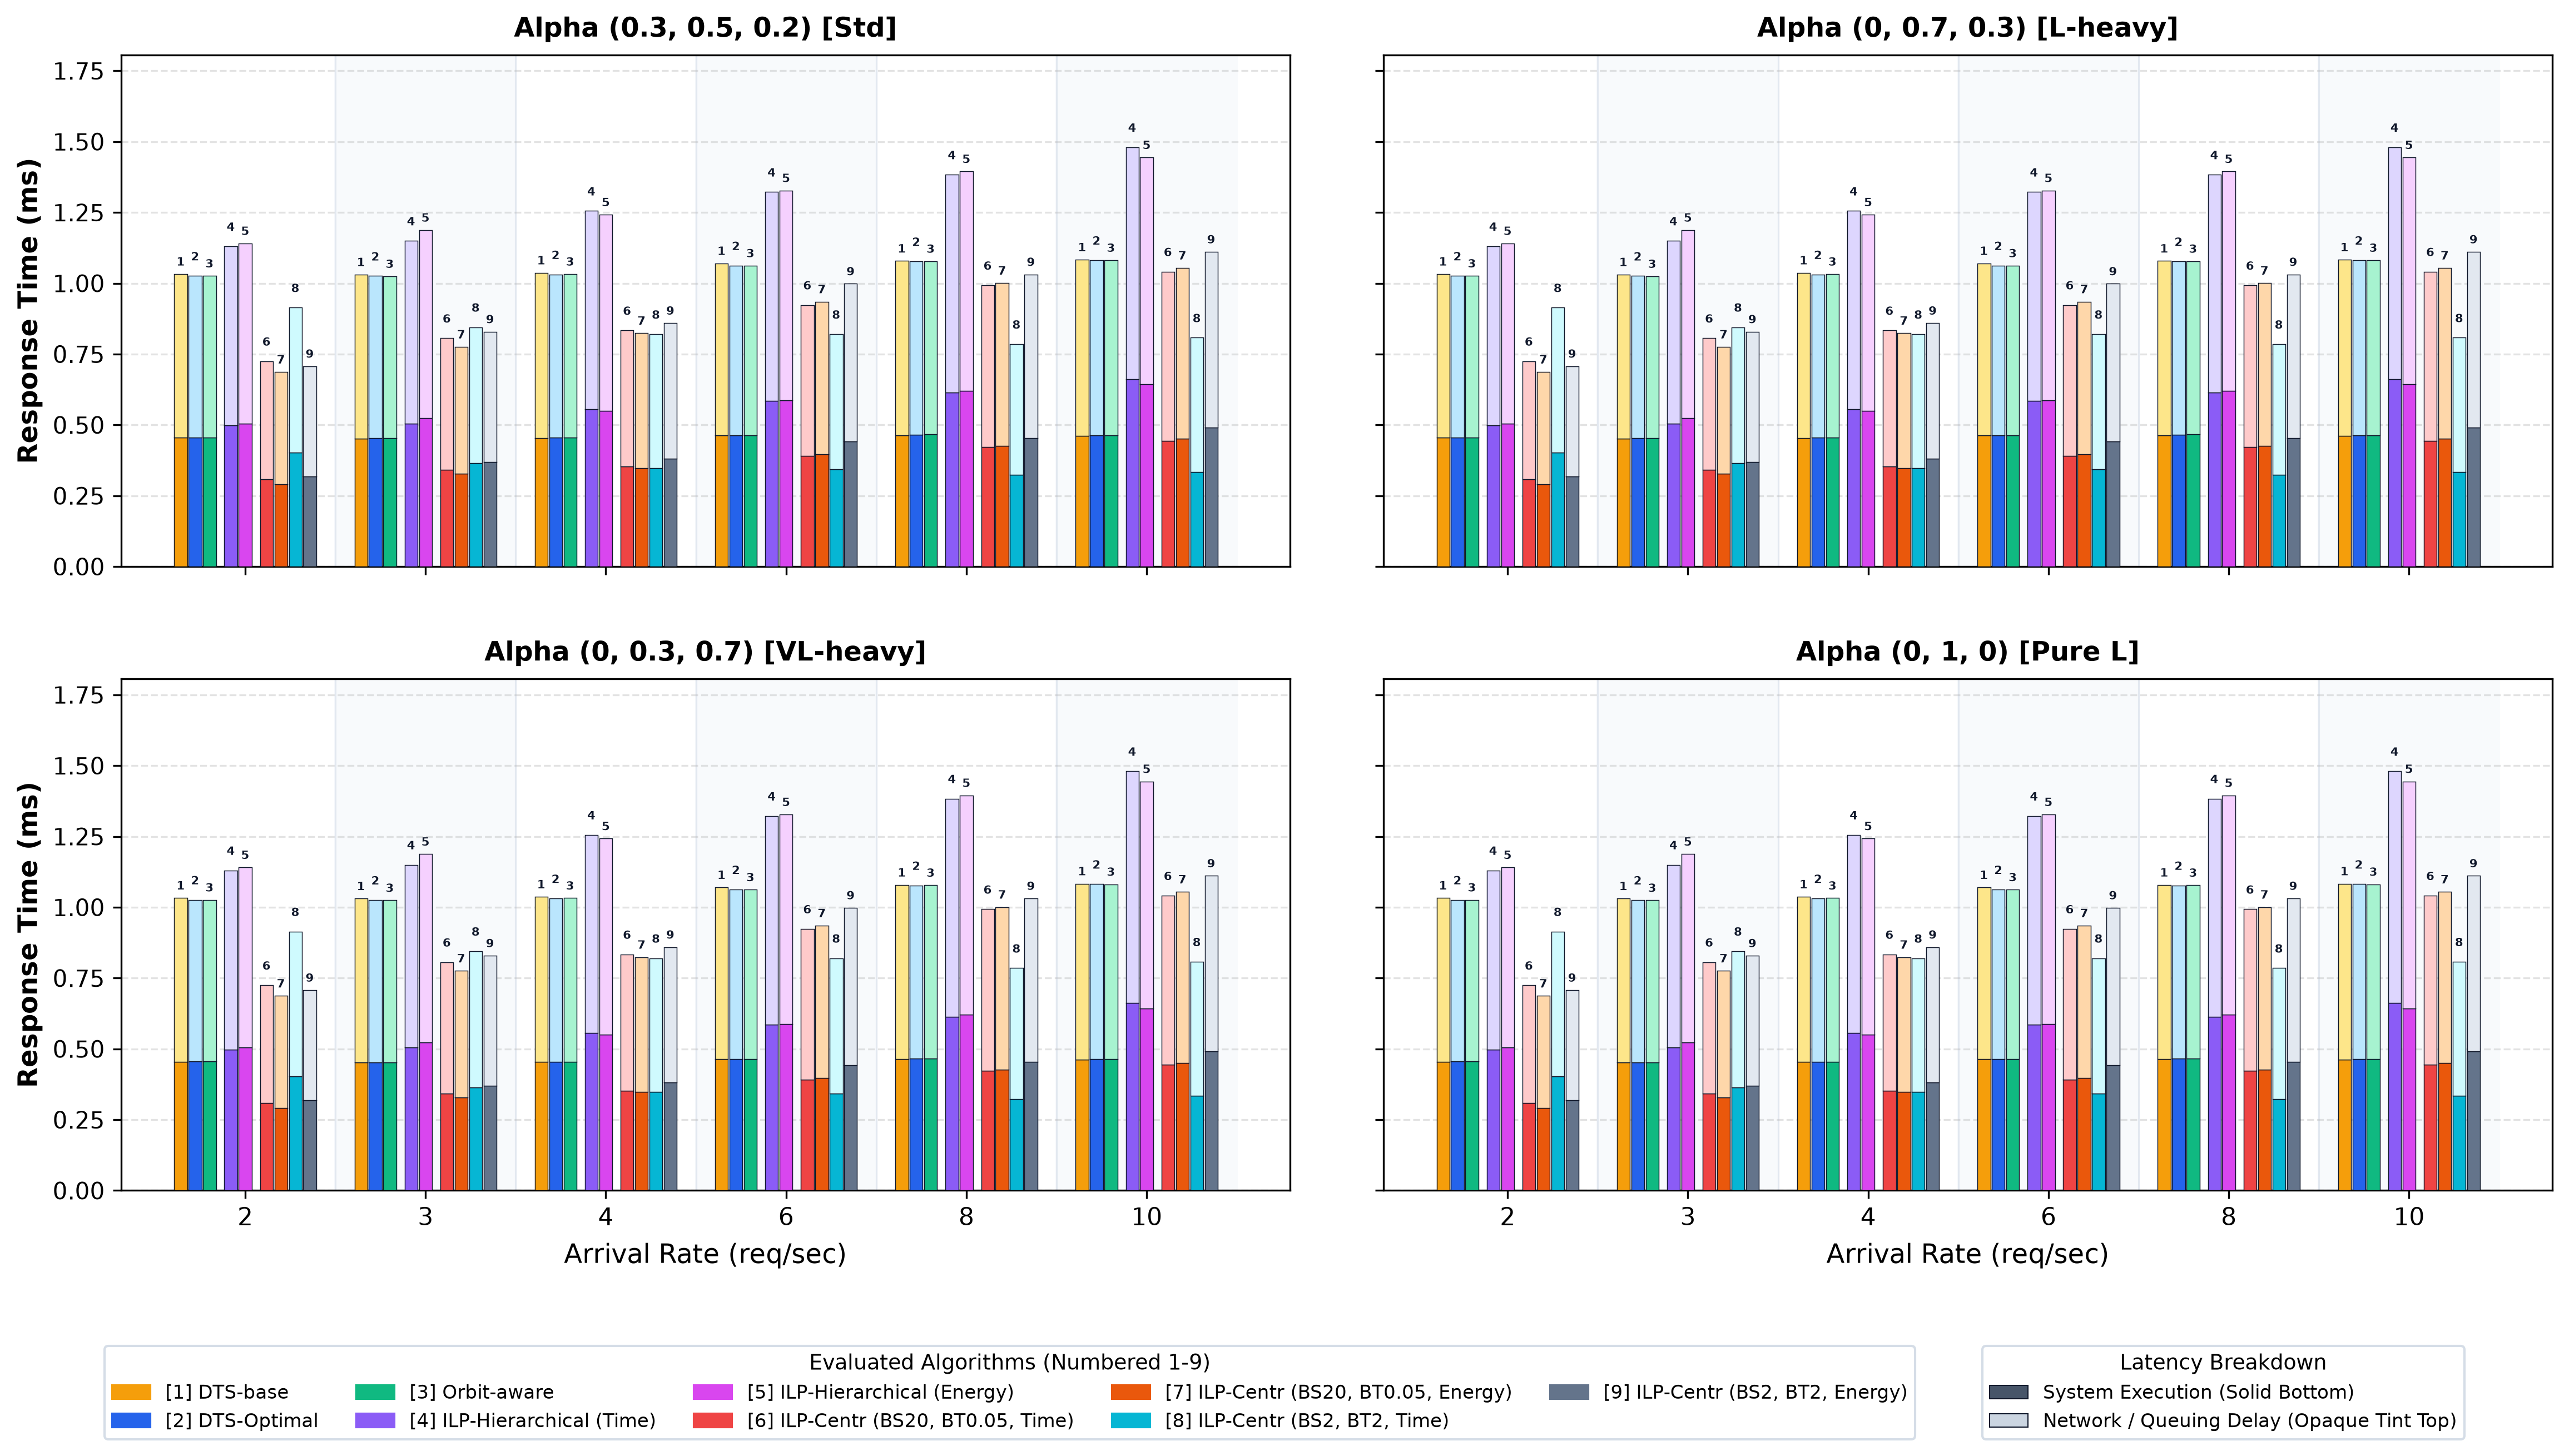
\includegraphics[width=\linewidth]{figures/02_Response_Time_Beta_0_1_0_40kJ.png} \\
        \vspace{0.3cm}
        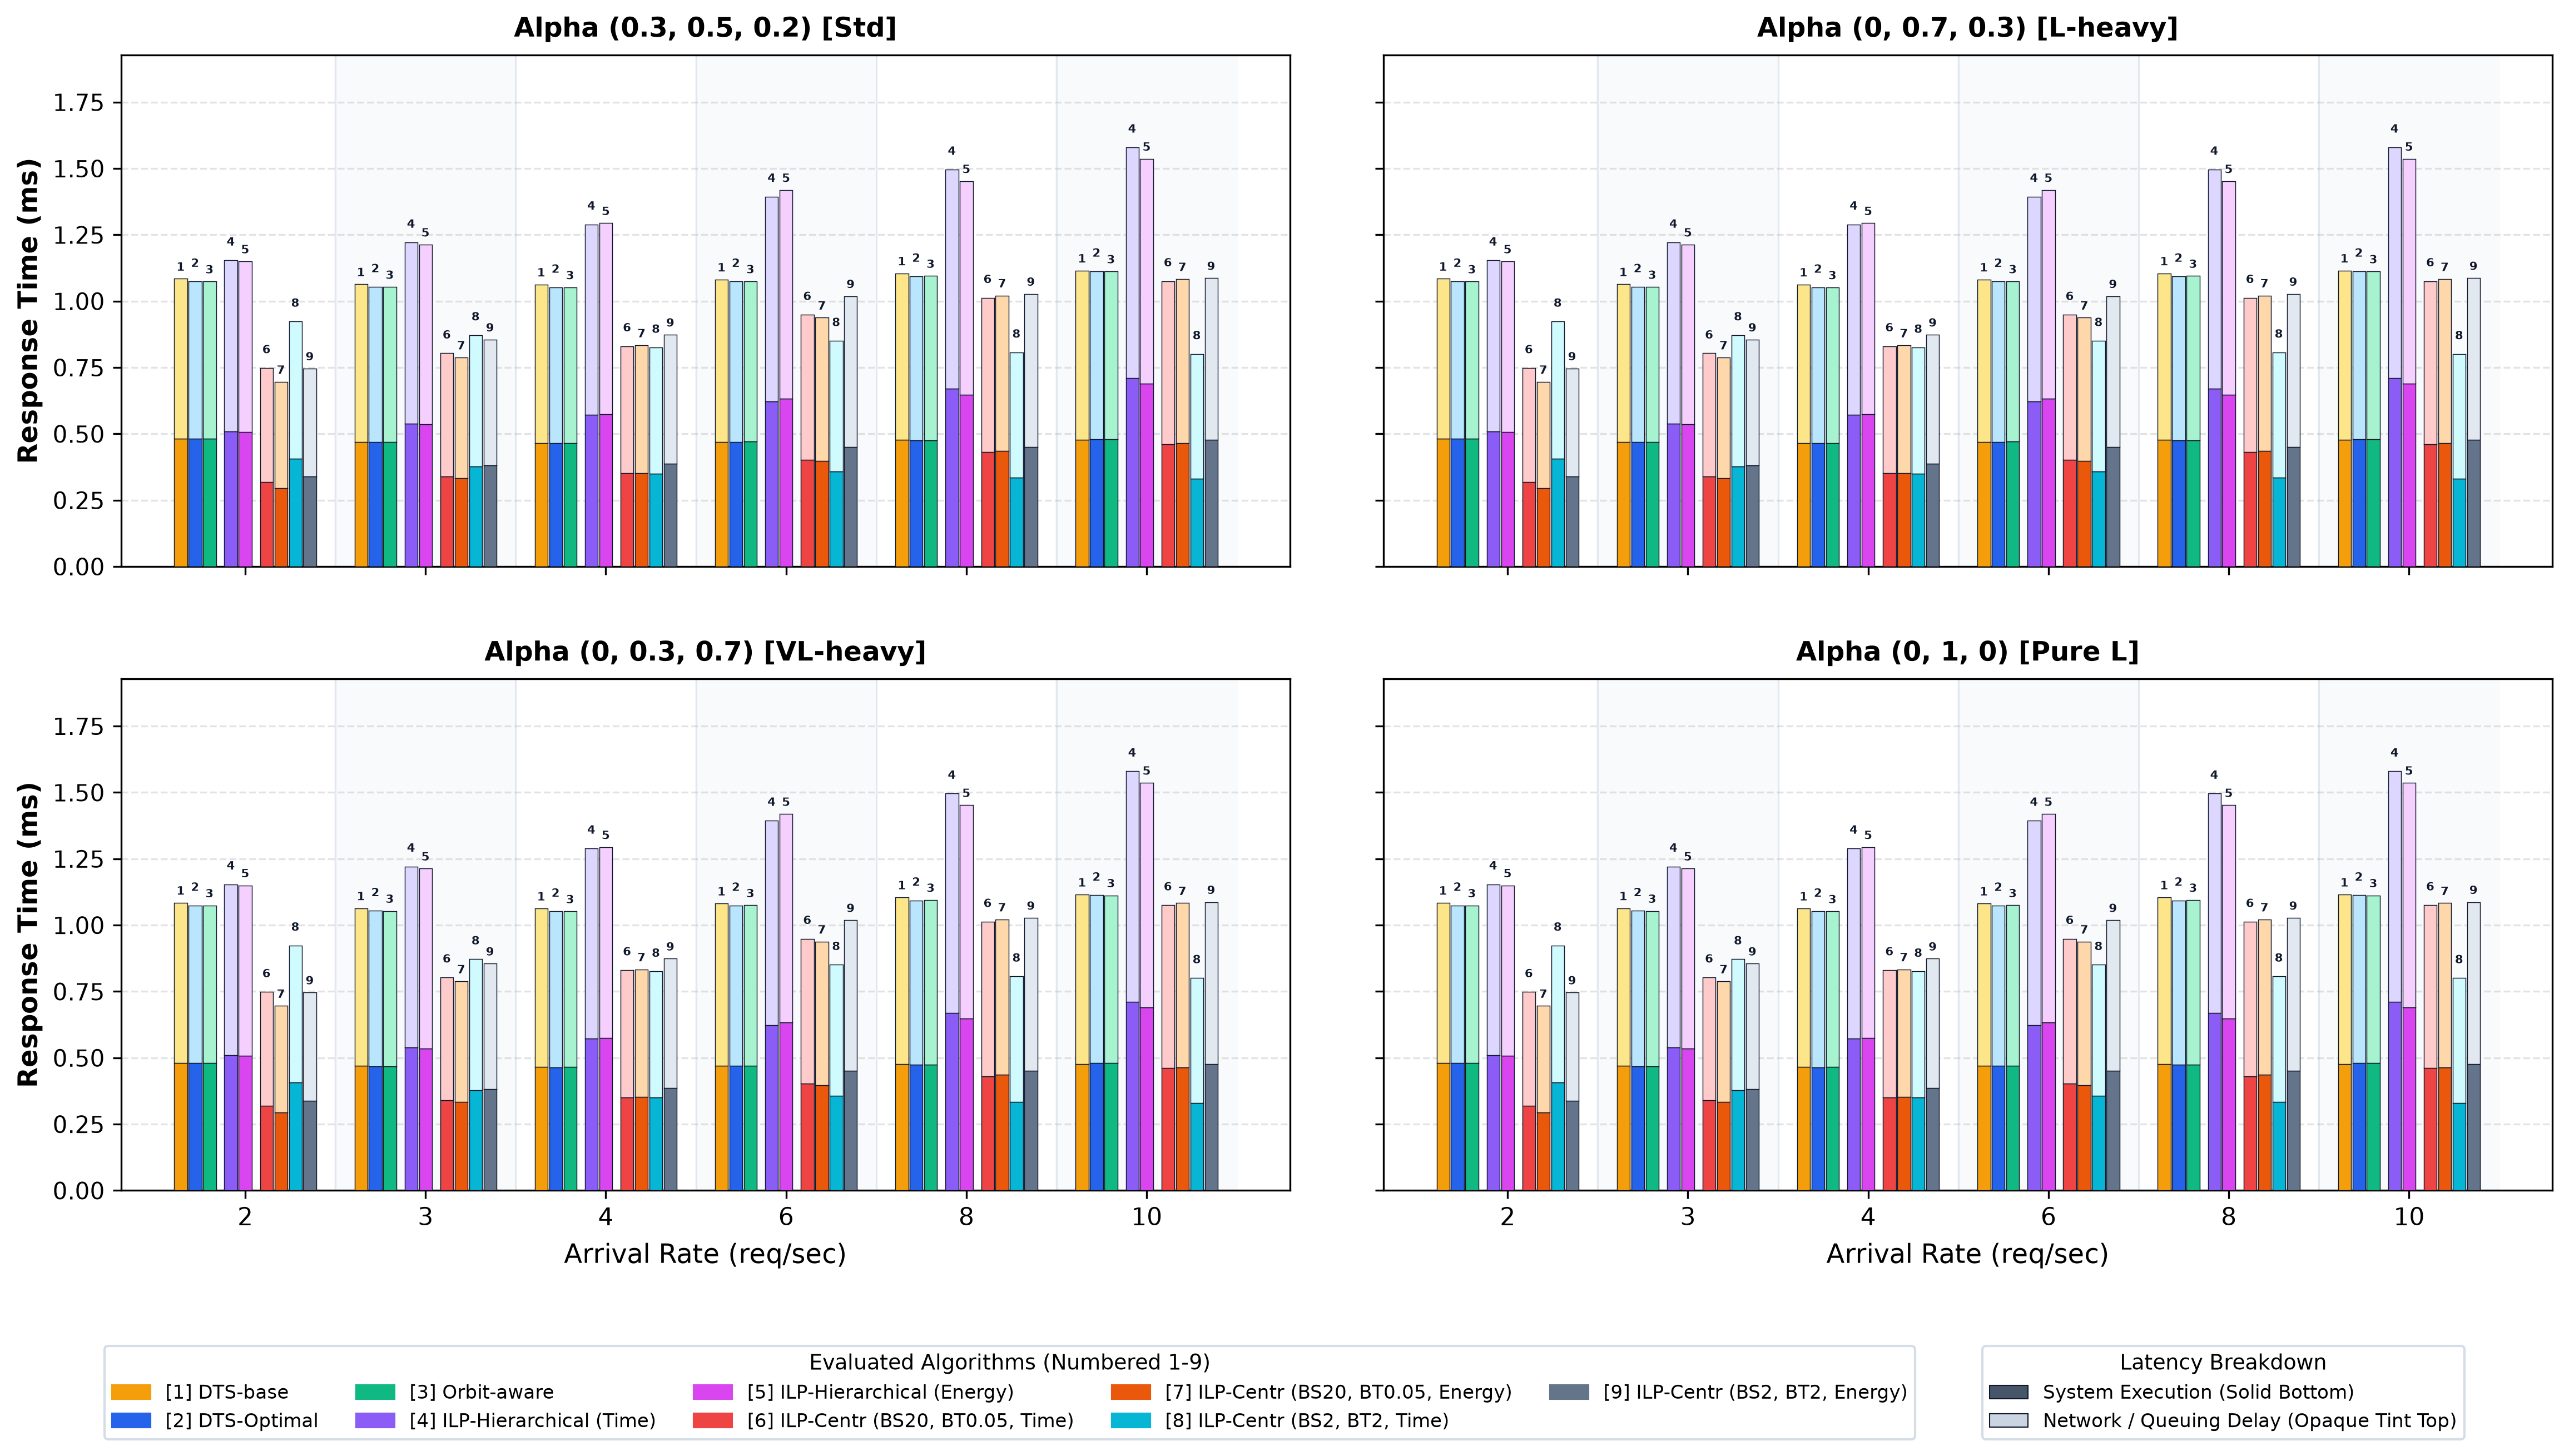
\includegraphics[width=\linewidth]{figures/02_Response_Time_Beta_0_1_0_80kJ.png}
        \caption{Response Time decomposition under CPU-Intensive Workload $\boldsymbol{\beta} = (0, 1, 0)$ showing the dominance of queuing latency under heavy computational load.}
        \label{fig:rt_cpu}
    \end{adjustwidth}
\end{figure}

\begin{figure}[H]
    \begin{adjustwidth}{-1.5cm}{-1.5cm}
        \centering
        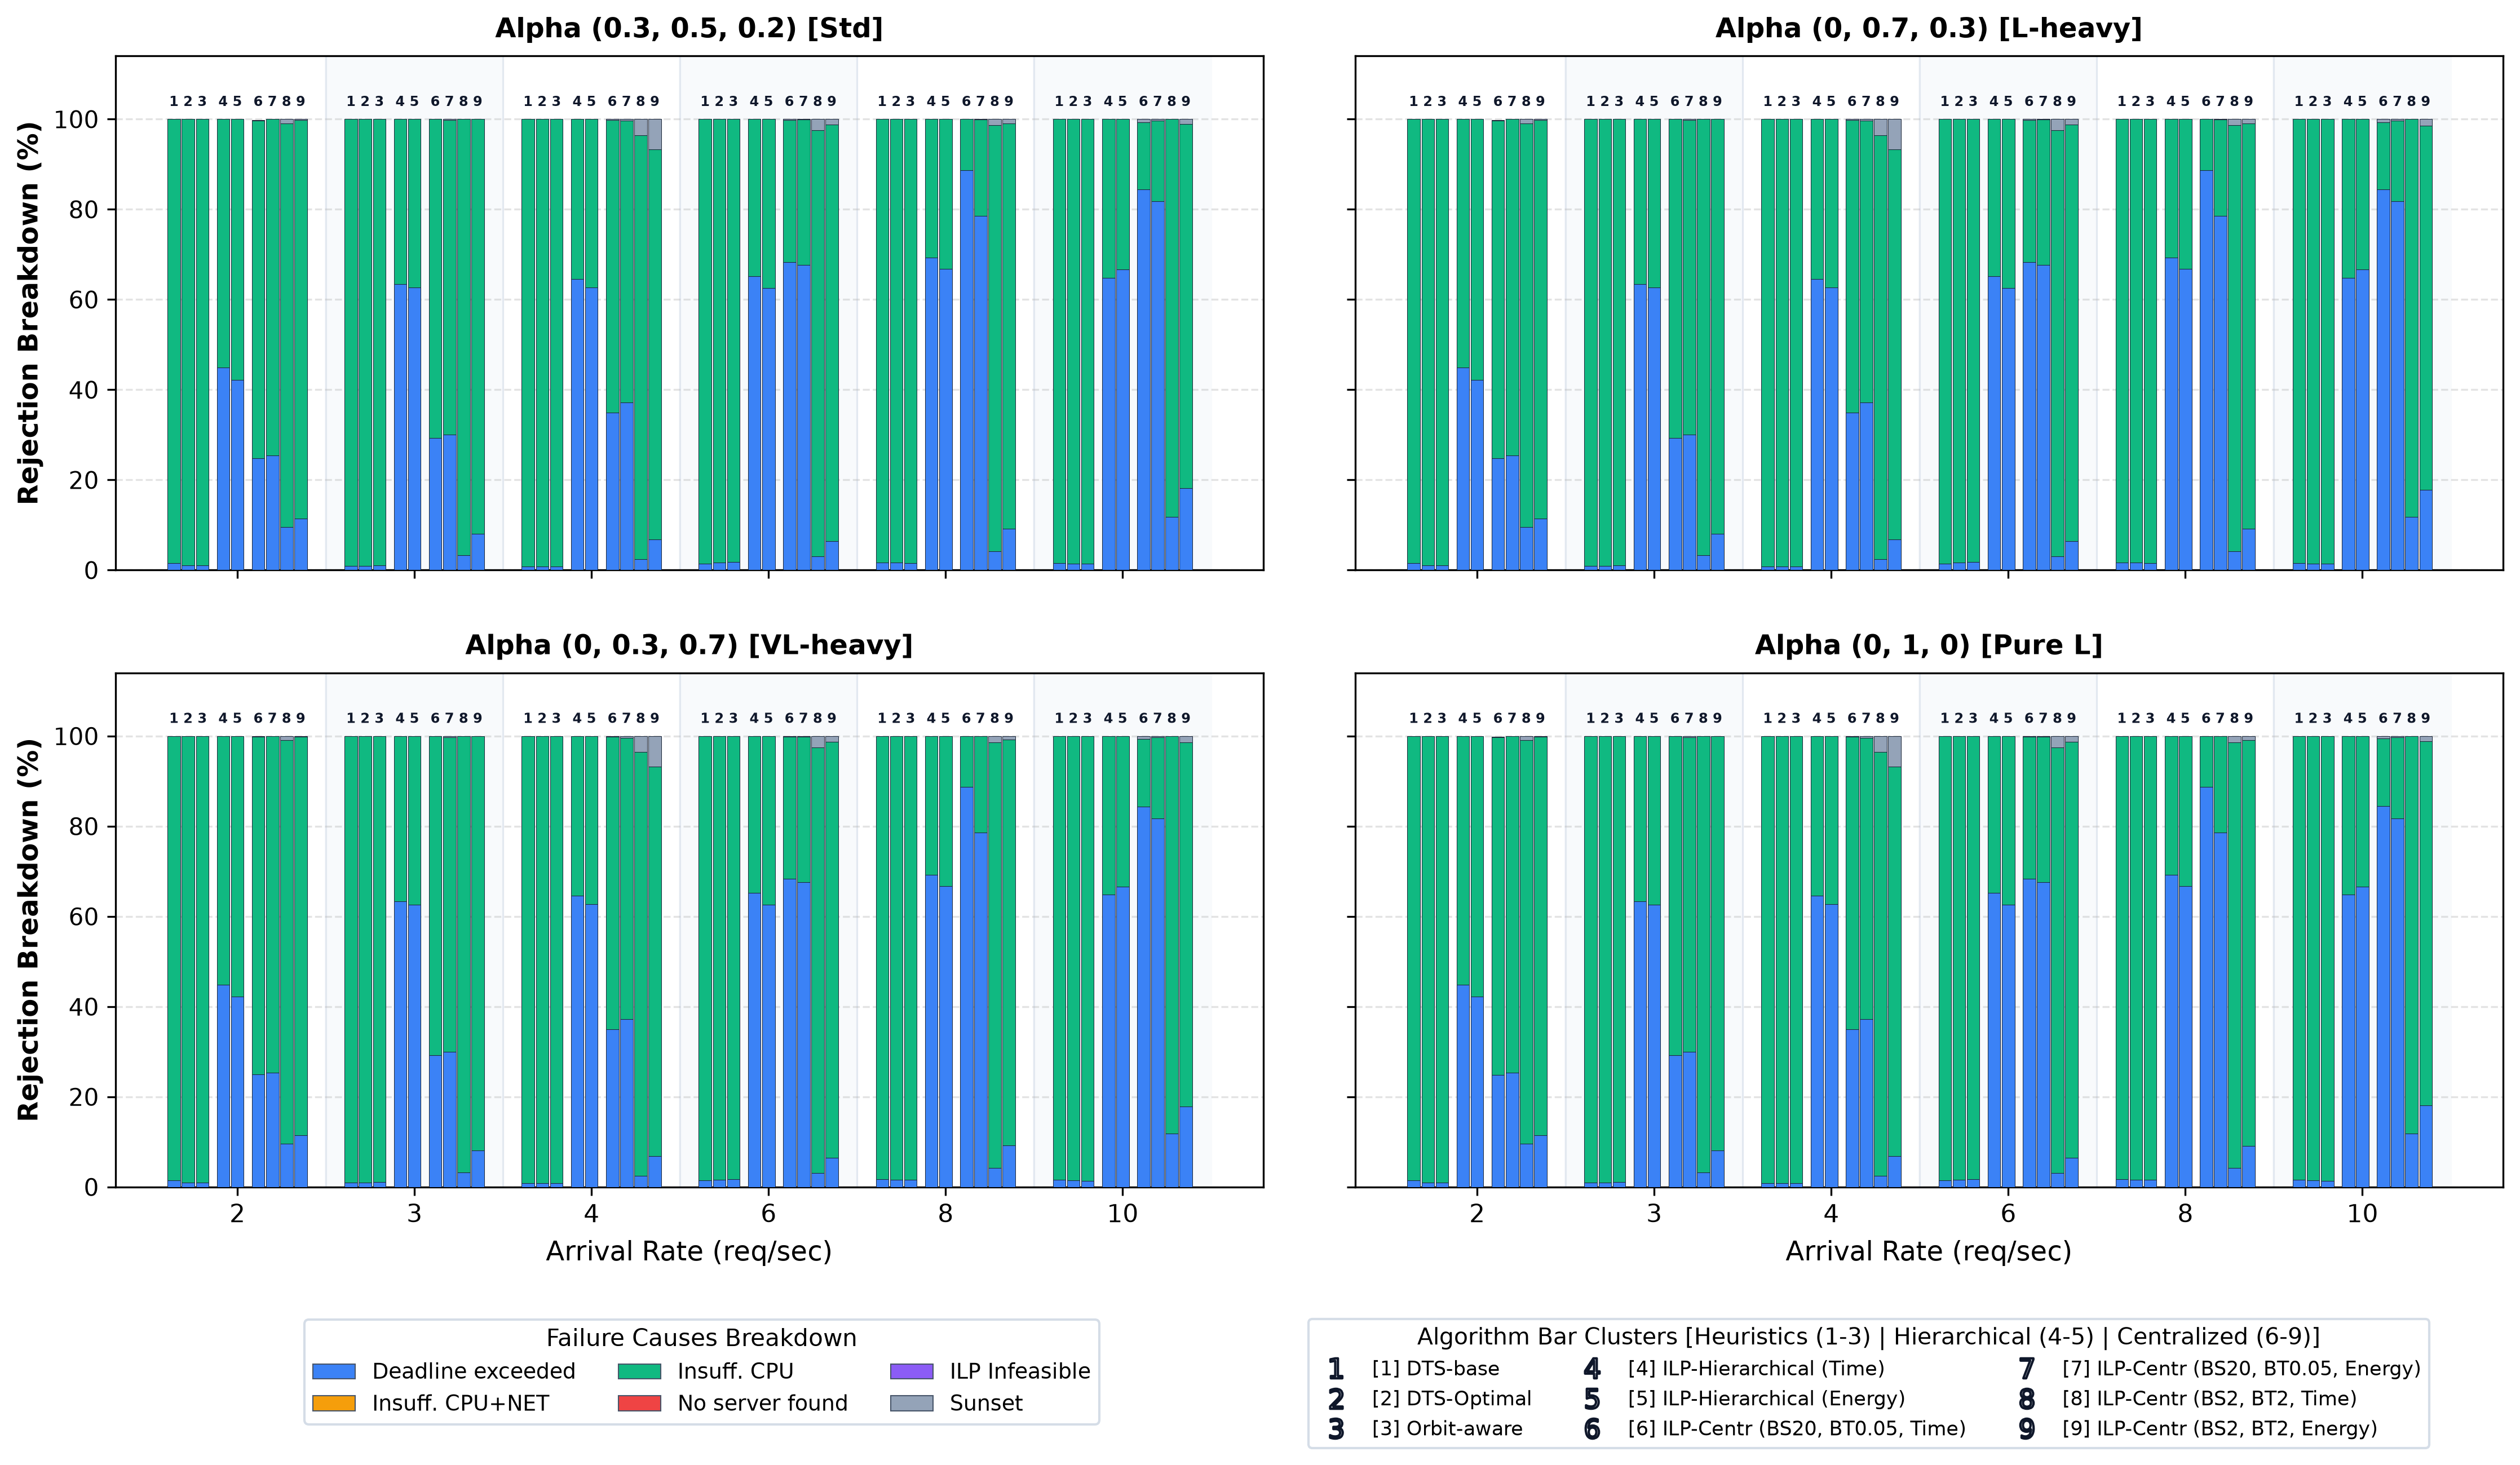
\includegraphics[width=\linewidth]{figures/03_Rejection_Causes_Beta_0_1_0_40kJ.png} \\
        \vspace{0.3cm}
        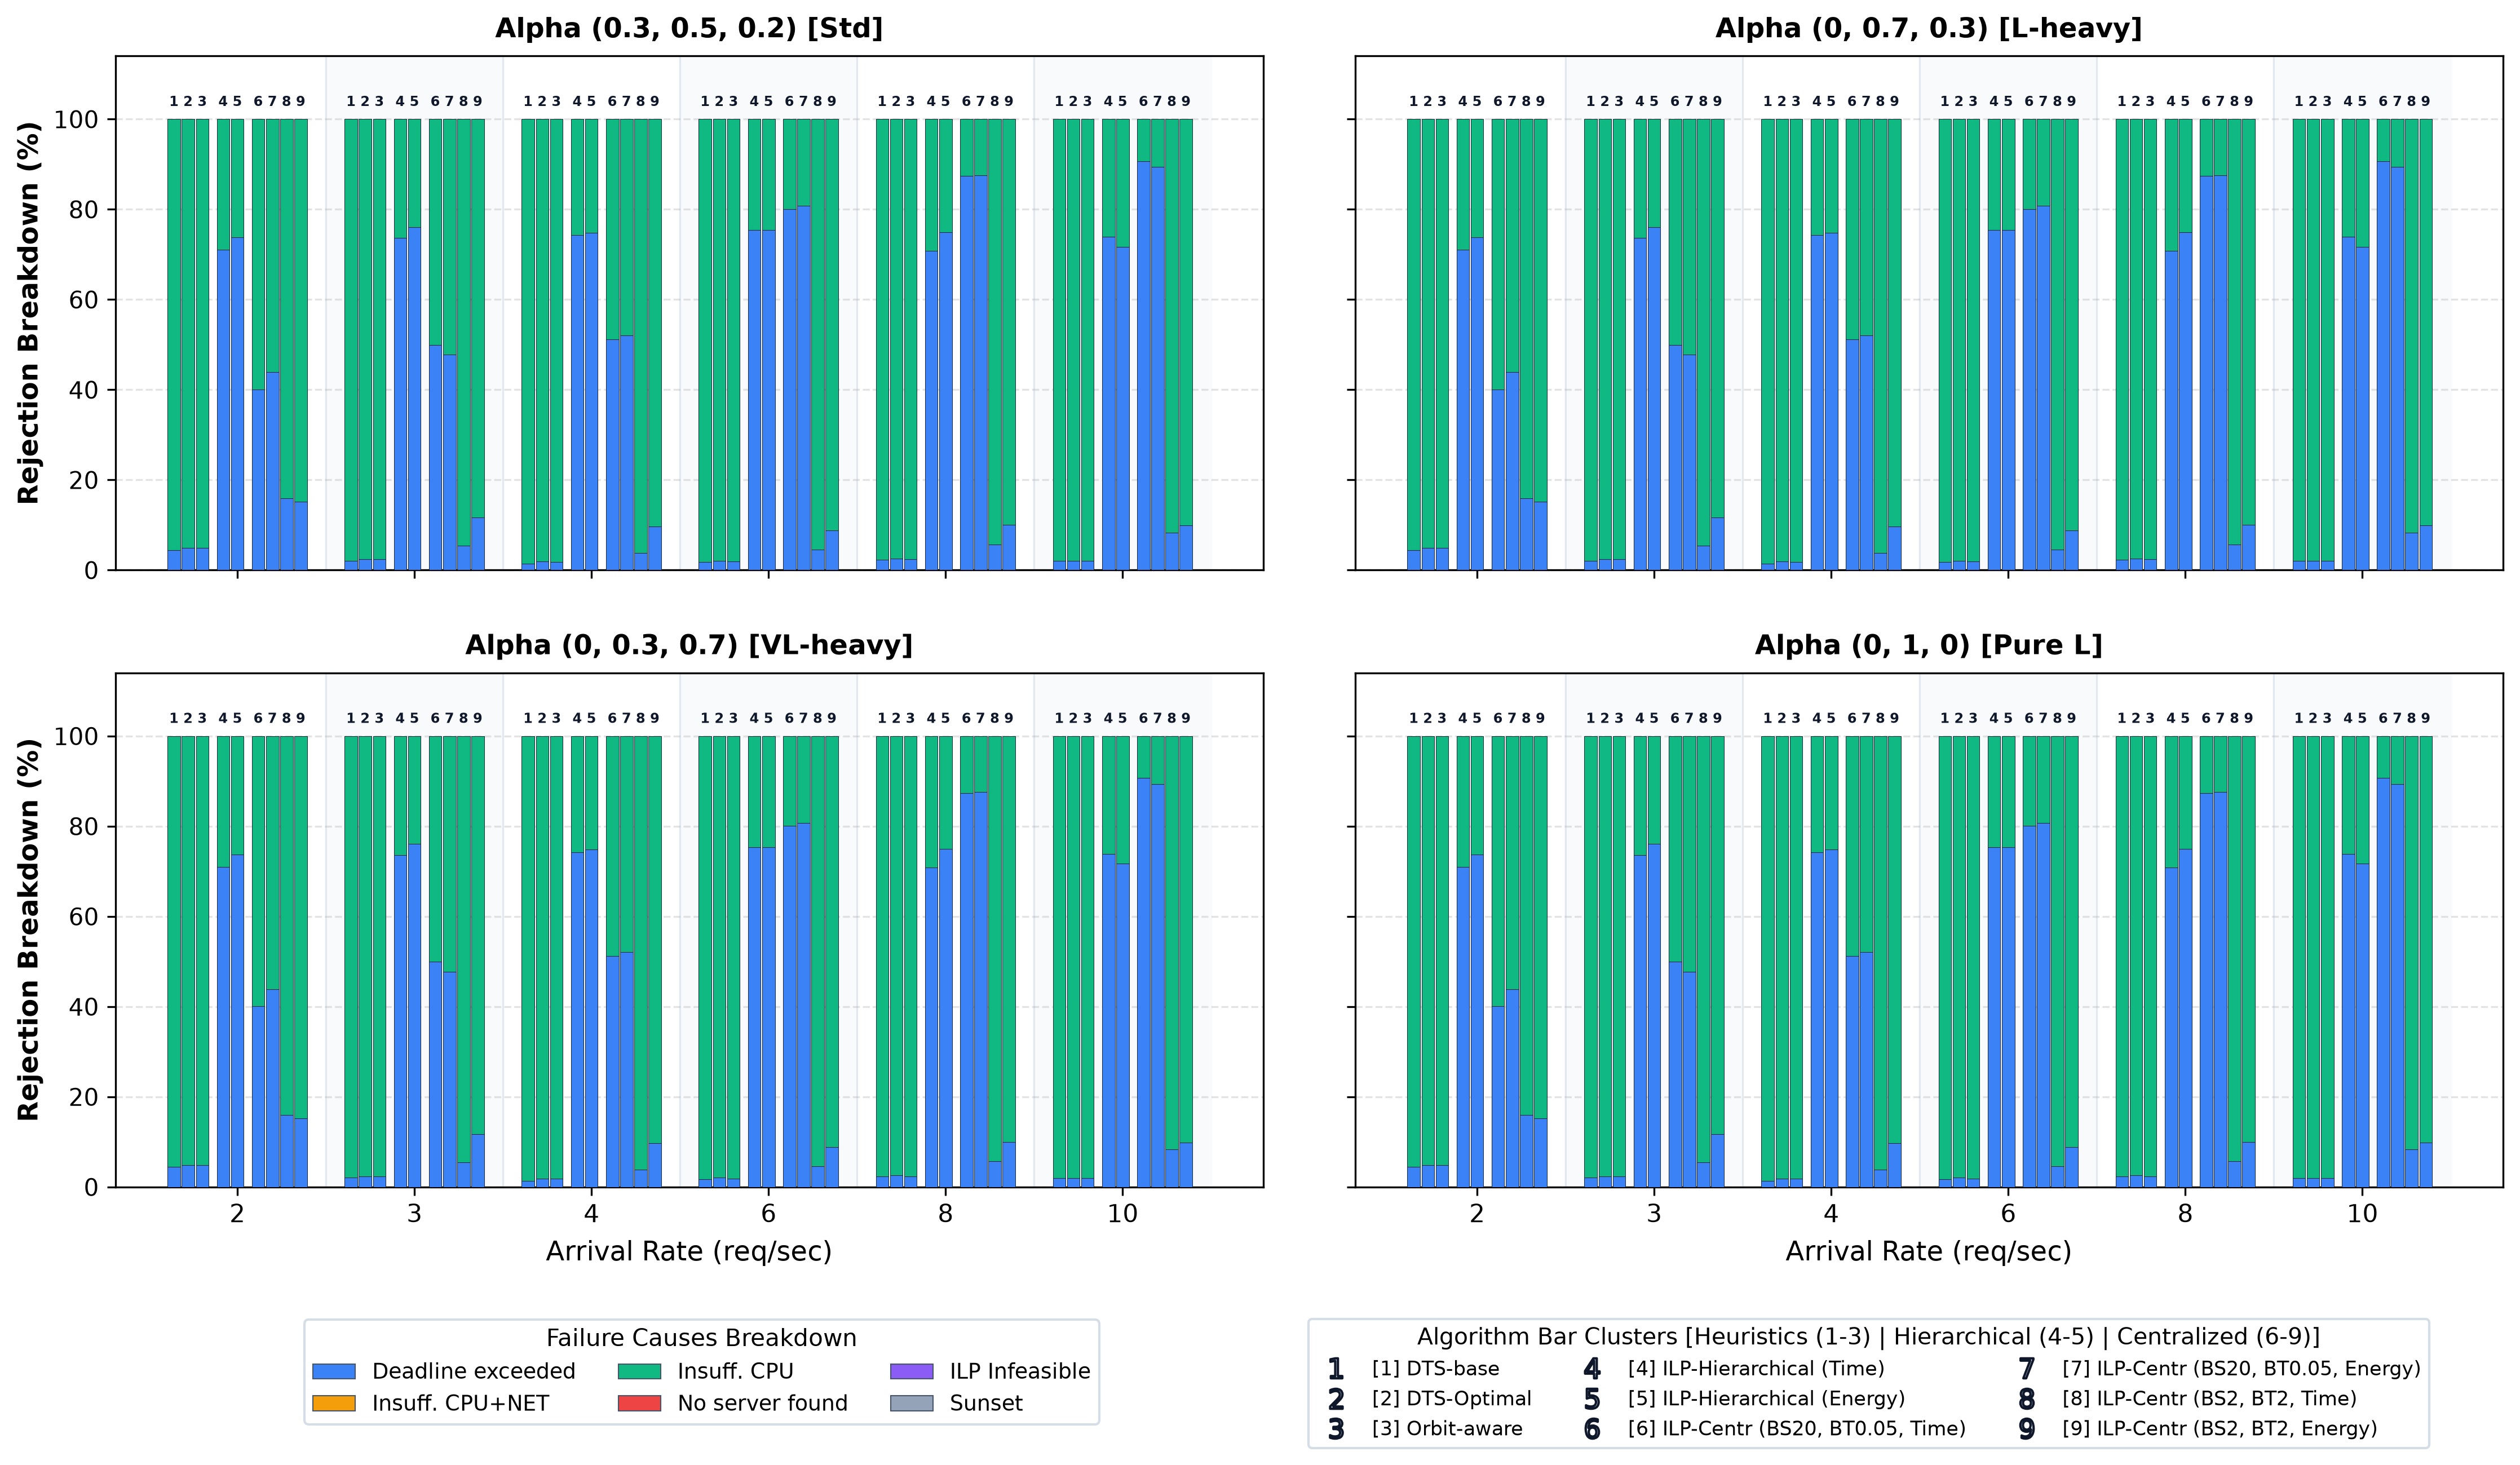
\includegraphics[width=\linewidth]{figures/03_Rejection_Causes_Beta_0_1_0_80kJ.png}
        \caption{Rejection Causes distribution under CPU-Intensive Workload $\boldsymbol{\beta} = (0, 1, 0)$, illustrating the sharp dichotomy between heuristic drops and optimization deadline timeouts.}
        \label{fig:rej_cpu}
    \end{adjustwidth}
\end{figure}

\subsubsection{Energy Inelasticity and Success Rate Dynamics}
The most prominent finding in the CPU-intensive profile is \textbf{inelasticity to energy budget scaling}. Comparing the 40~kJ (top) and 80~kJ (bottom) charts in Figure~\ref{fig:sr_cpu} reveals virtually identical curves. Because the payload sizes are minimal, optical transmission consumes negligible power. The system bottleneck is strictly governed by SEN processor queues. Here, heuristics demonstrate remarkable resilience ($\approx 75\%$ at peak load), while all optimization models collapse below $30\%$ at $\lambda = 10\text{ req/s}$ due to extreme temporal congestion.

\subsubsection{The Fundamental Rejection Dichotomy}
Figure~\ref{fig:rej_cpu} presents the most profound architectural insight of the benchmark, revealing a binary divergence in failure causes:
\begin{itemize}
    \item \textbf{Distributed Heuristics:} Exactly \textbf{$100\%$ of all task rejections} are caused by \textit{Insufficient CPU} (green bars). Because heuristics evaluate nodes greedily with zero ingress buffering, if a satellite's CPU core is occupied, the task is dropped immediately. Not a single task fails due to \textit{Deadline Exceeded}.
    \item \textbf{Optimization Models:} The vast majority of rejections ($70\%\text{--}90\%$) are caused by \textbf{\textit{Deadline Exceeded}} (blue bars). Under heavy computational demands, processor queues expand across all satellites. When the ILP solver aggregates tasks, the cumulative waiting delay renders the end-to-end latency constraint mathematically infeasible. Tasks fail not because the constellation lacks physical transceivers, but because temporal queueing violates rigid application deadlines before tasks can be dispatched to SENs.
\end{itemize}

% -----------------------------------------------------------------------------
% SUBSECTION 5.2.3: DATA-INTENSIVE WORKLOAD
% -----------------------------------------------------------------------------
\subsection{Communication-Heavy Stress: Data-Intensive Profile (\texorpdfstring{$\boldsymbol{\beta} = (0, 0, 1)$}{beta = (0, 0, 1)})}
\label{subsec:bench_data}

In the data-intensive regime ($\boldsymbol{\beta} = (0, 0, 1)$), requests combine the transfer of massive data payloads ($20\text{--}50\text{ MB}$ governed by $\boldsymbol{\alpha}$) across multi-hop ISL routes, severely testing optical transceivers and energy depletion.

\begin{figure}[H]
    \begin{adjustwidth}{-1.5cm}{-1.5cm}
        \centering
        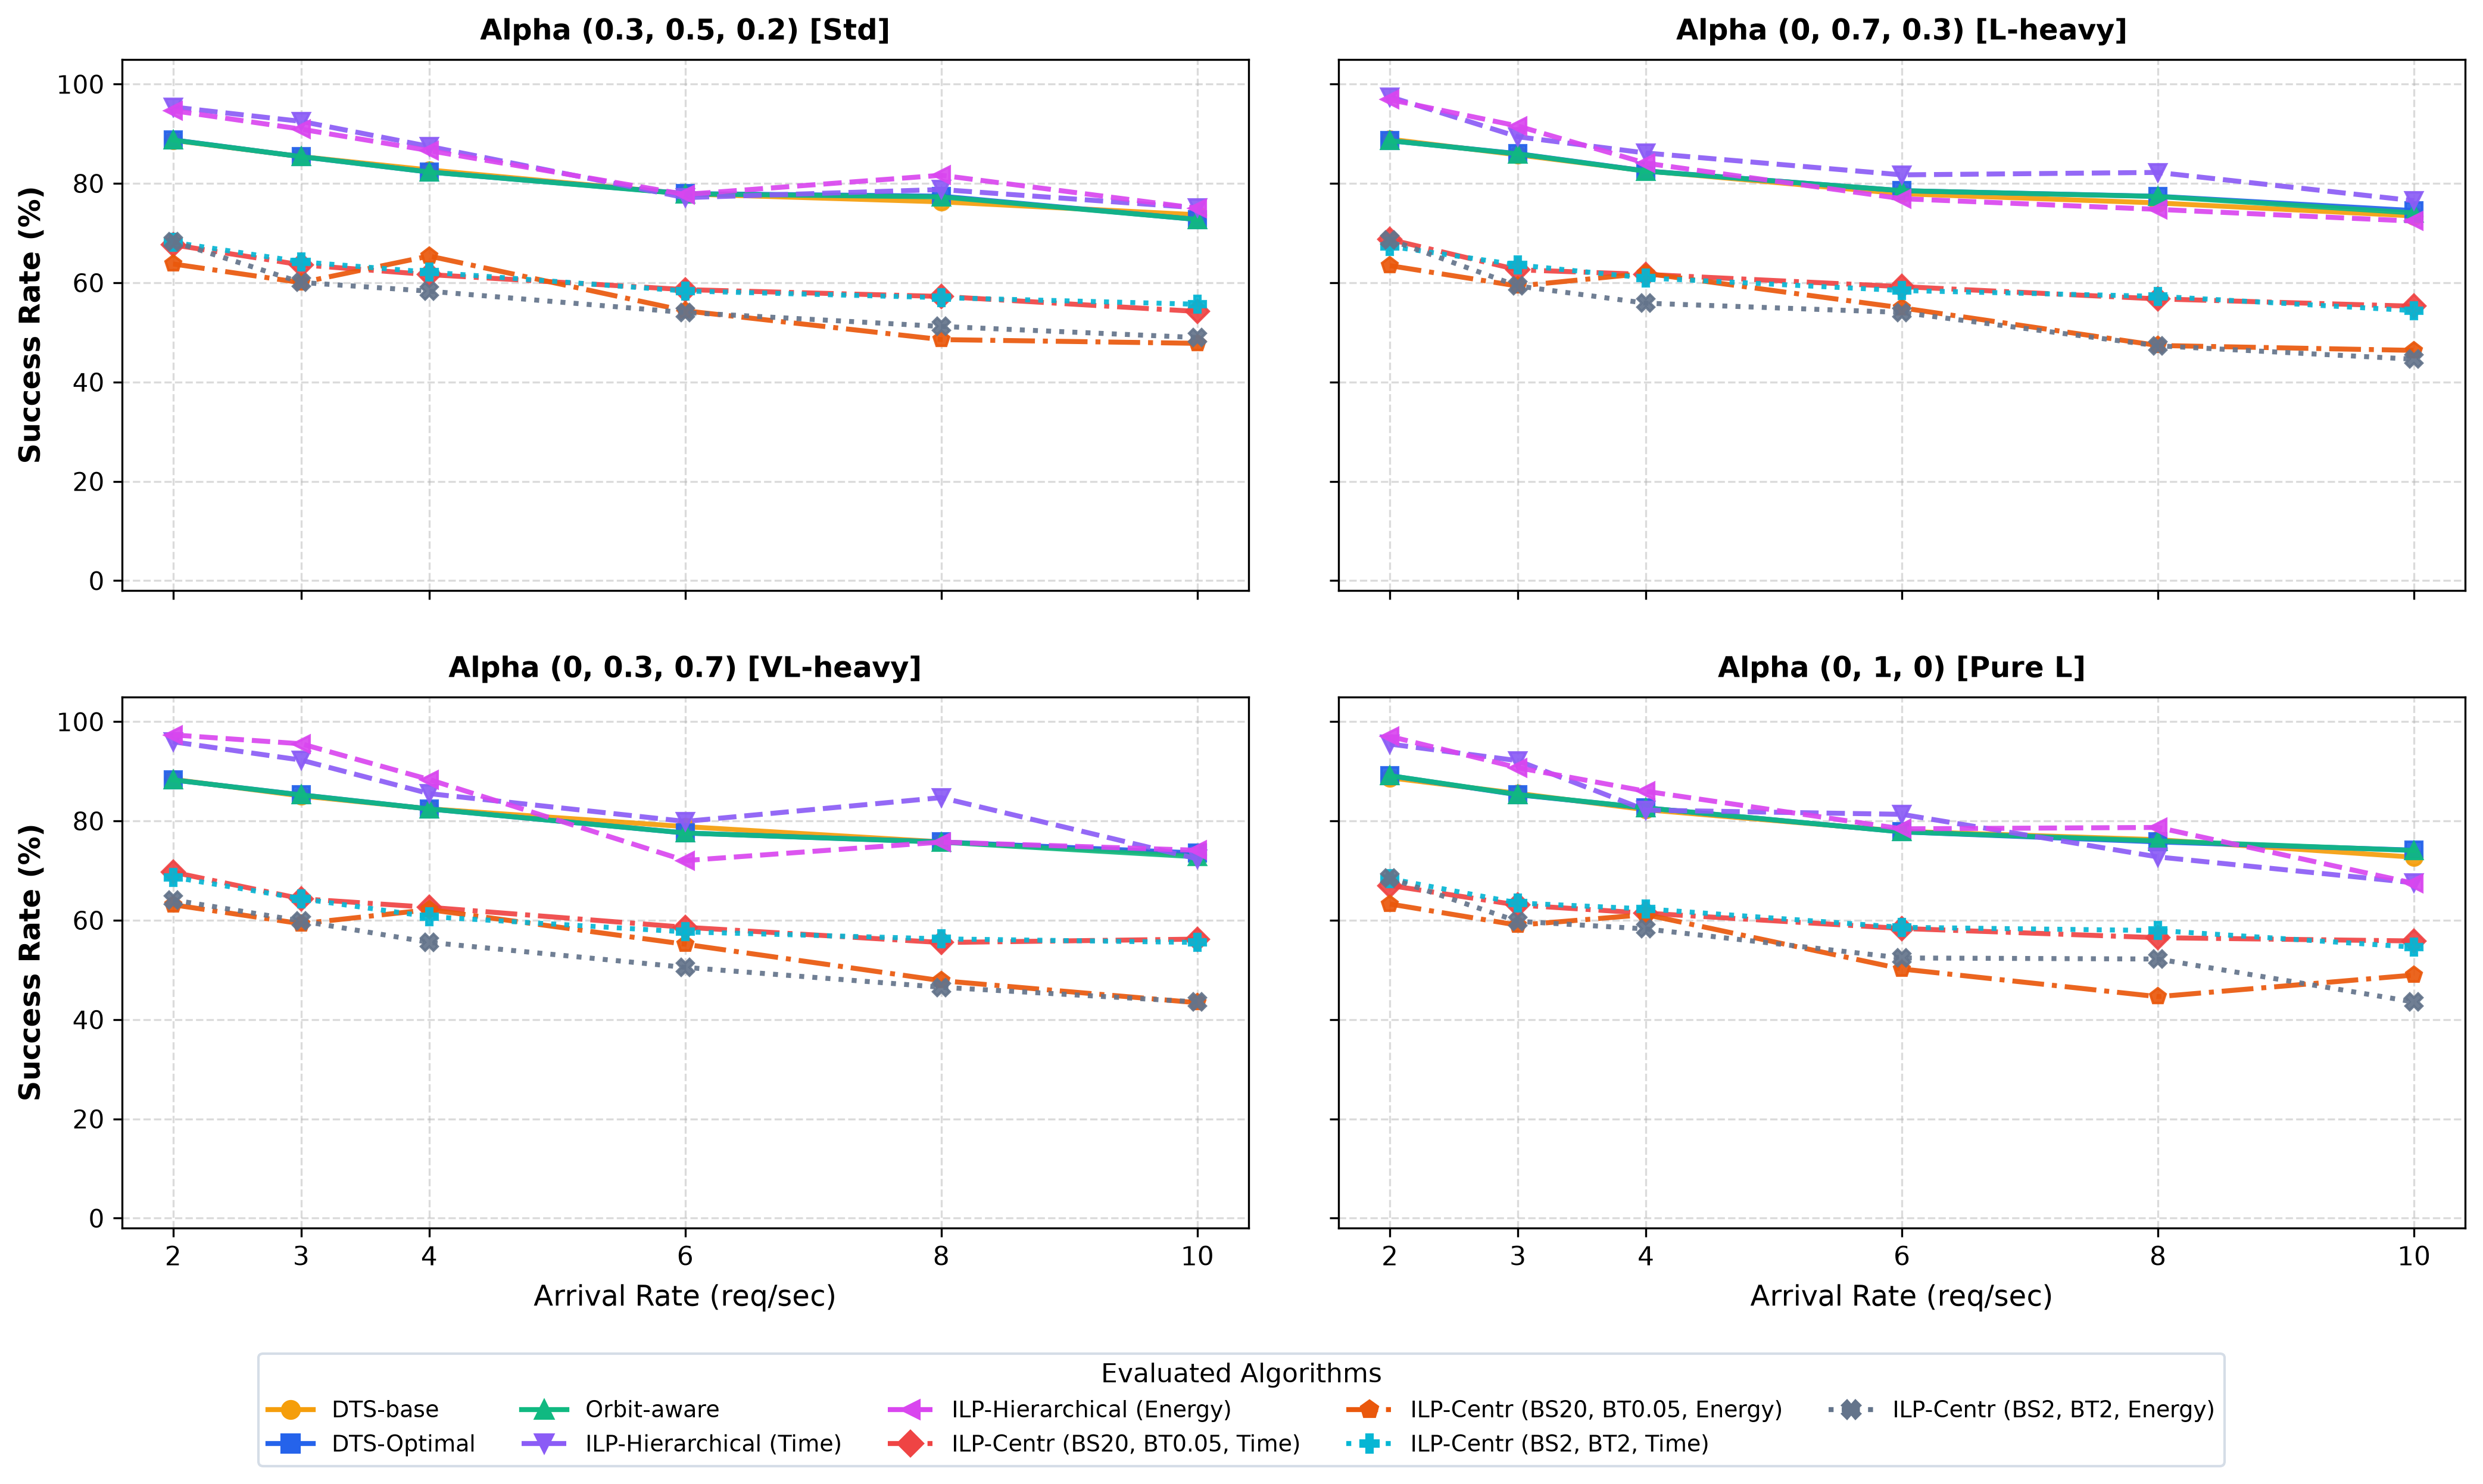
\includegraphics[width=\linewidth]{figures/01_Success_Rate_Beta_0_0_1_40kJ.png} \\
        \vspace{0.3cm}
        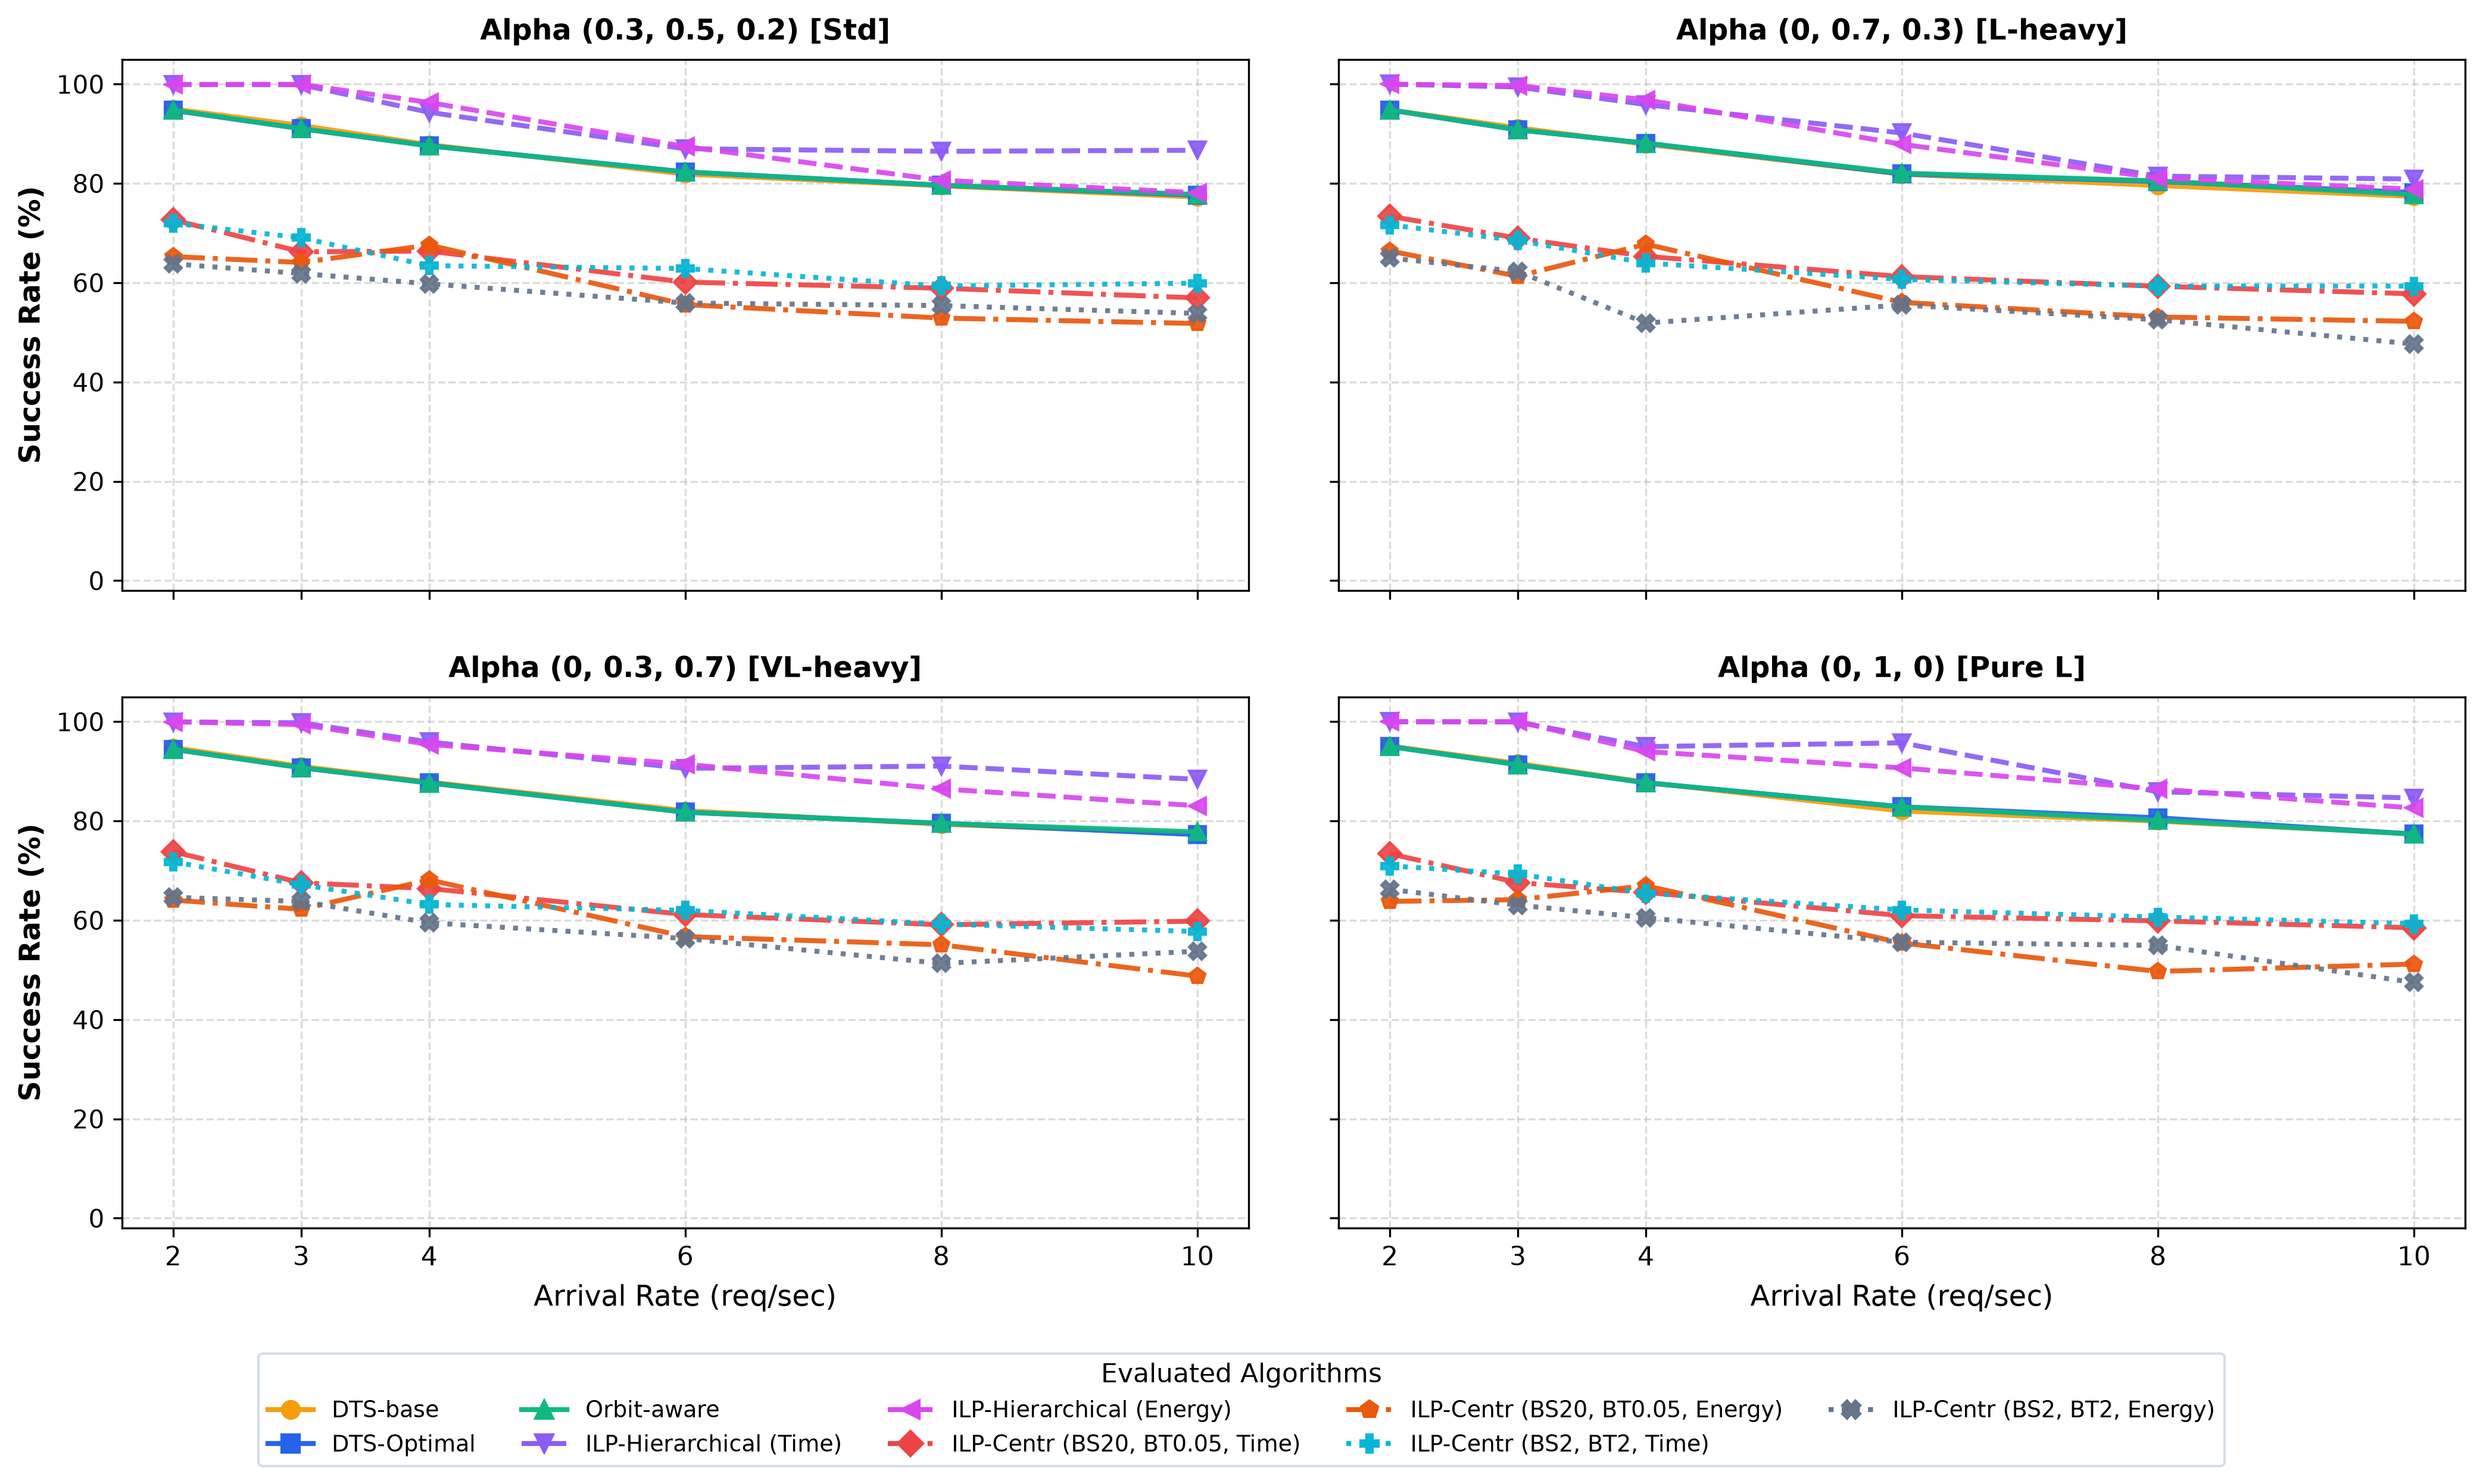
\includegraphics[width=\linewidth]{figures/01_Success_Rate_Beta_0_0_1_80kJ.png}
        \caption{Success Rate across arrival rates under Data-Intensive Workload $\boldsymbol{\beta} = (0, 0, 1)$ for $40\text{ kJ}$ (top) and $80\text{ kJ}$ (bottom) across payload distributions $\boldsymbol{\alpha}$.}
        \label{fig:sr_data}
    \end{adjustwidth}
\end{figure}

\begin{figure}[H]
    \begin{adjustwidth}{-1.5cm}{-1.5cm}
        \centering
        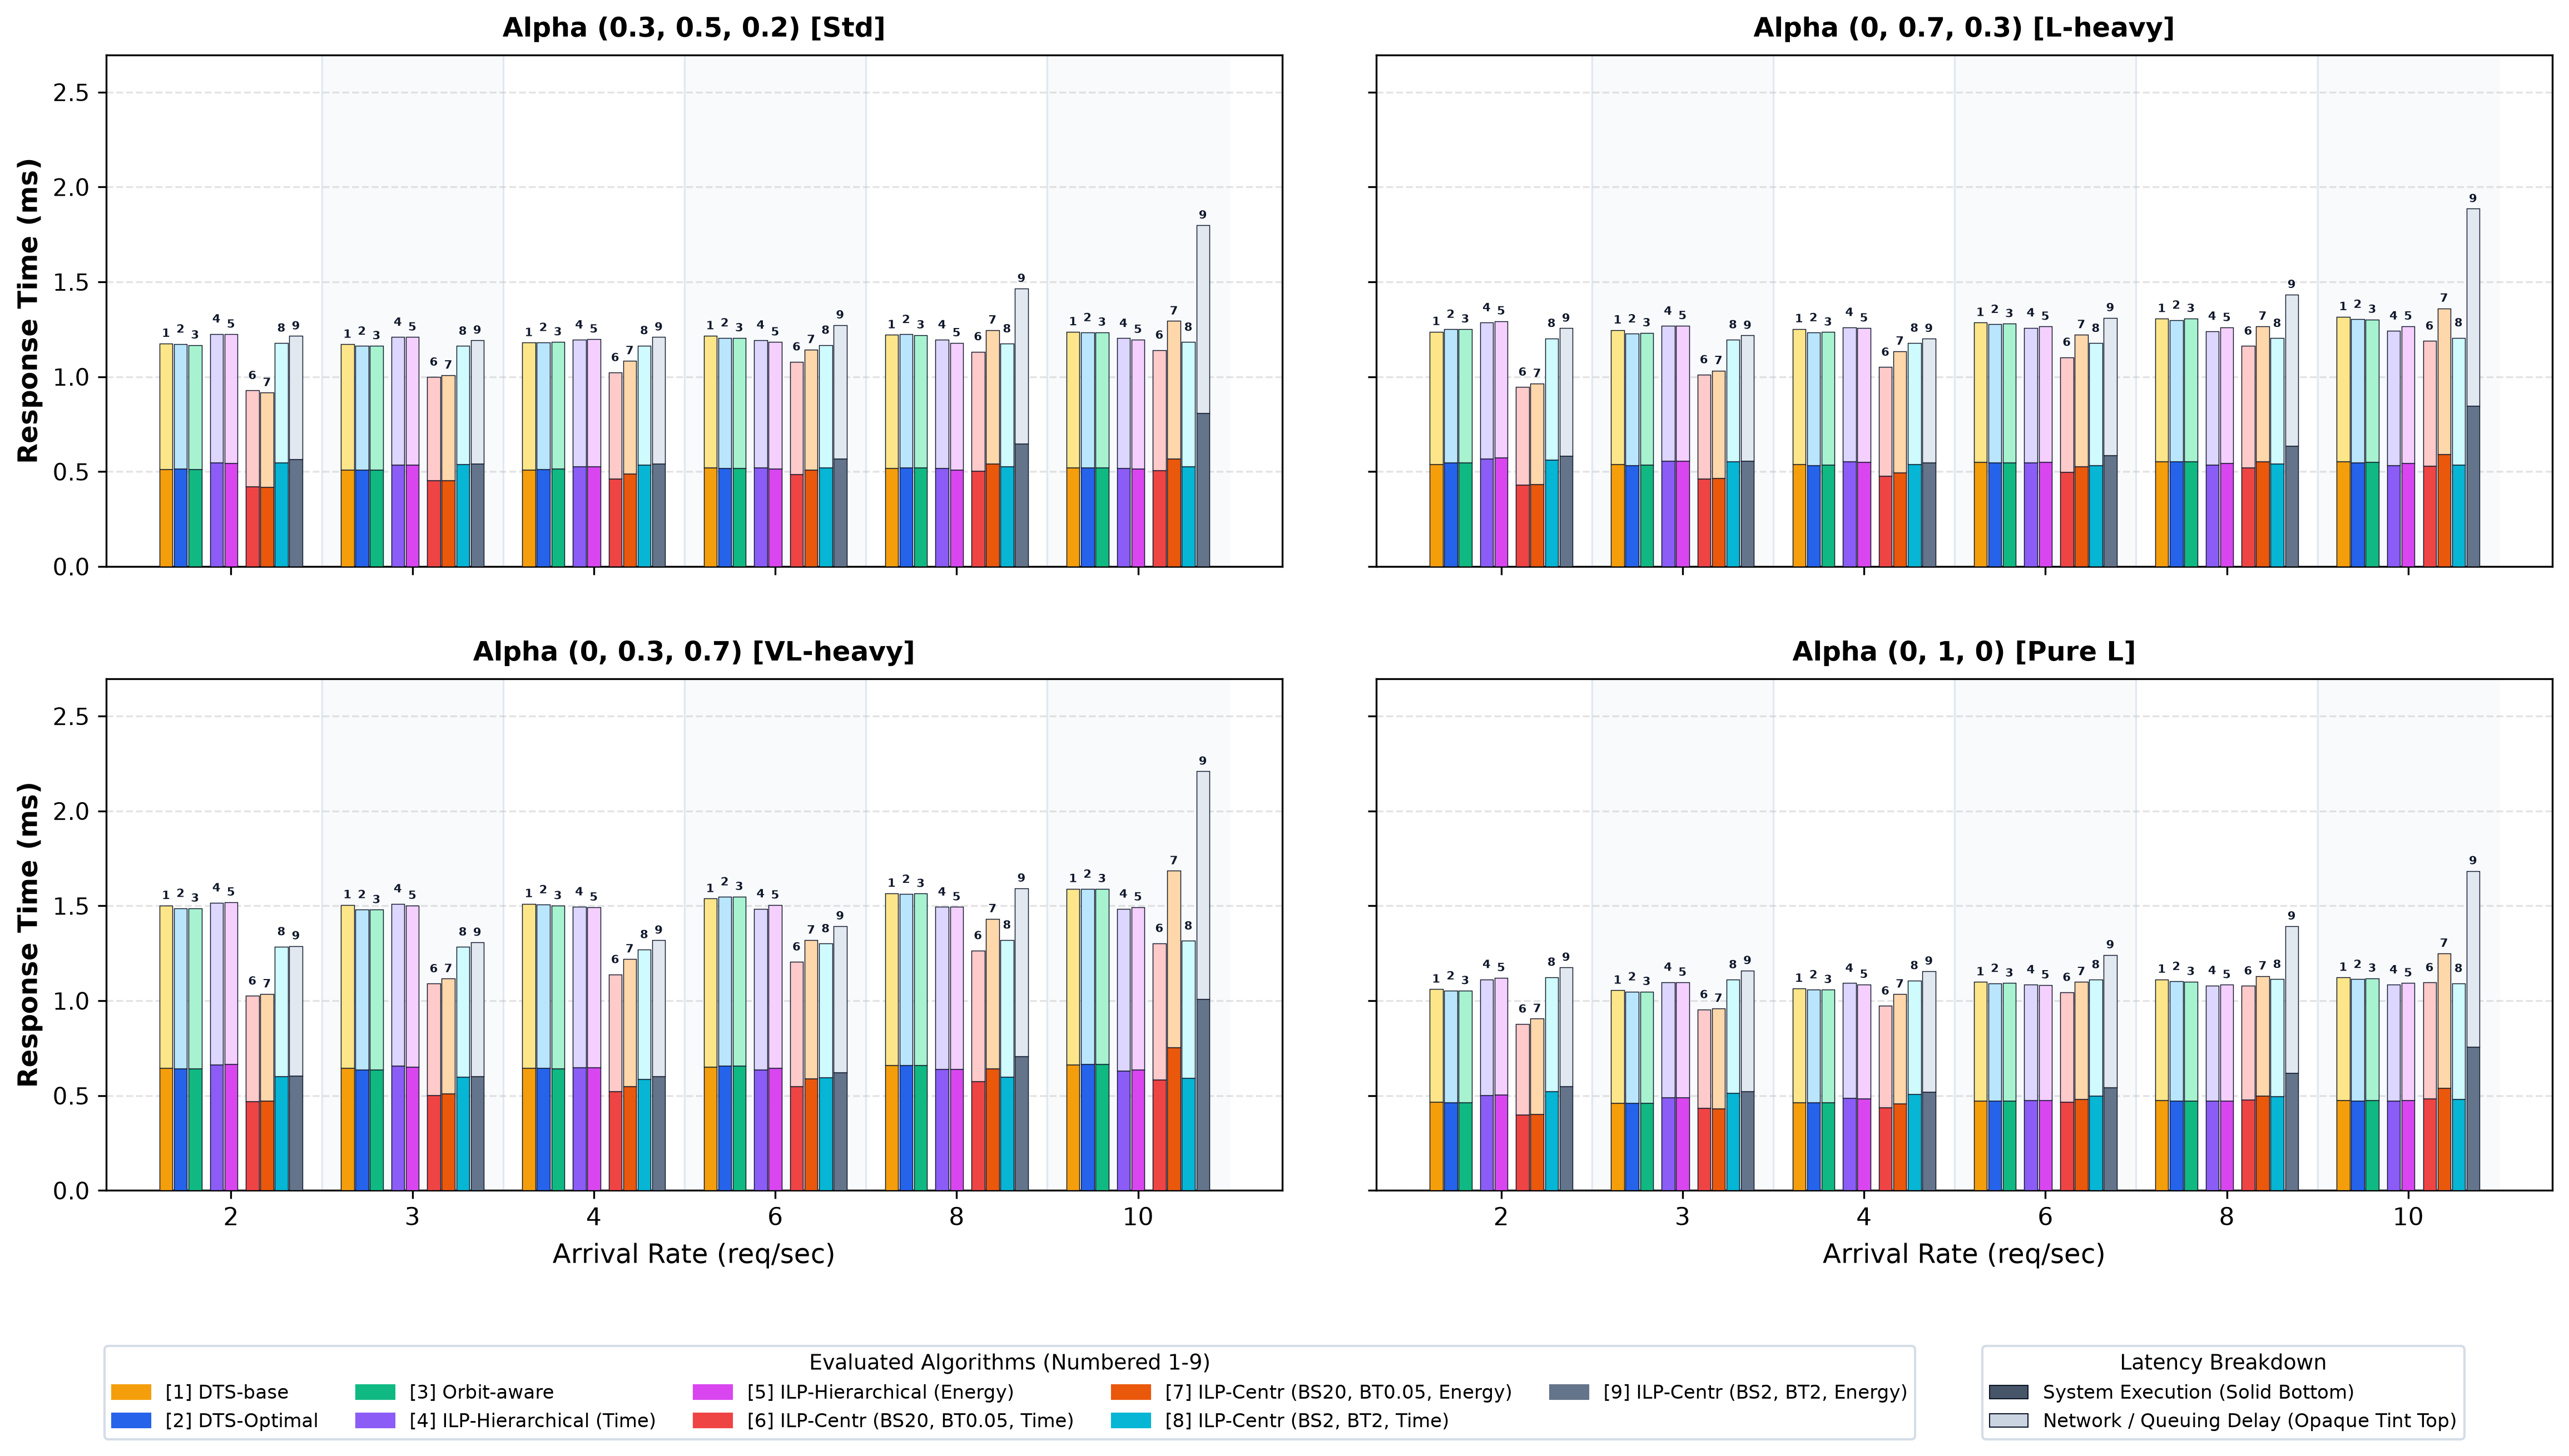
\includegraphics[width=\linewidth]{figures/02_Response_Time_Beta_0_0_1_40kJ.png} \\
        \vspace{0.3cm}
        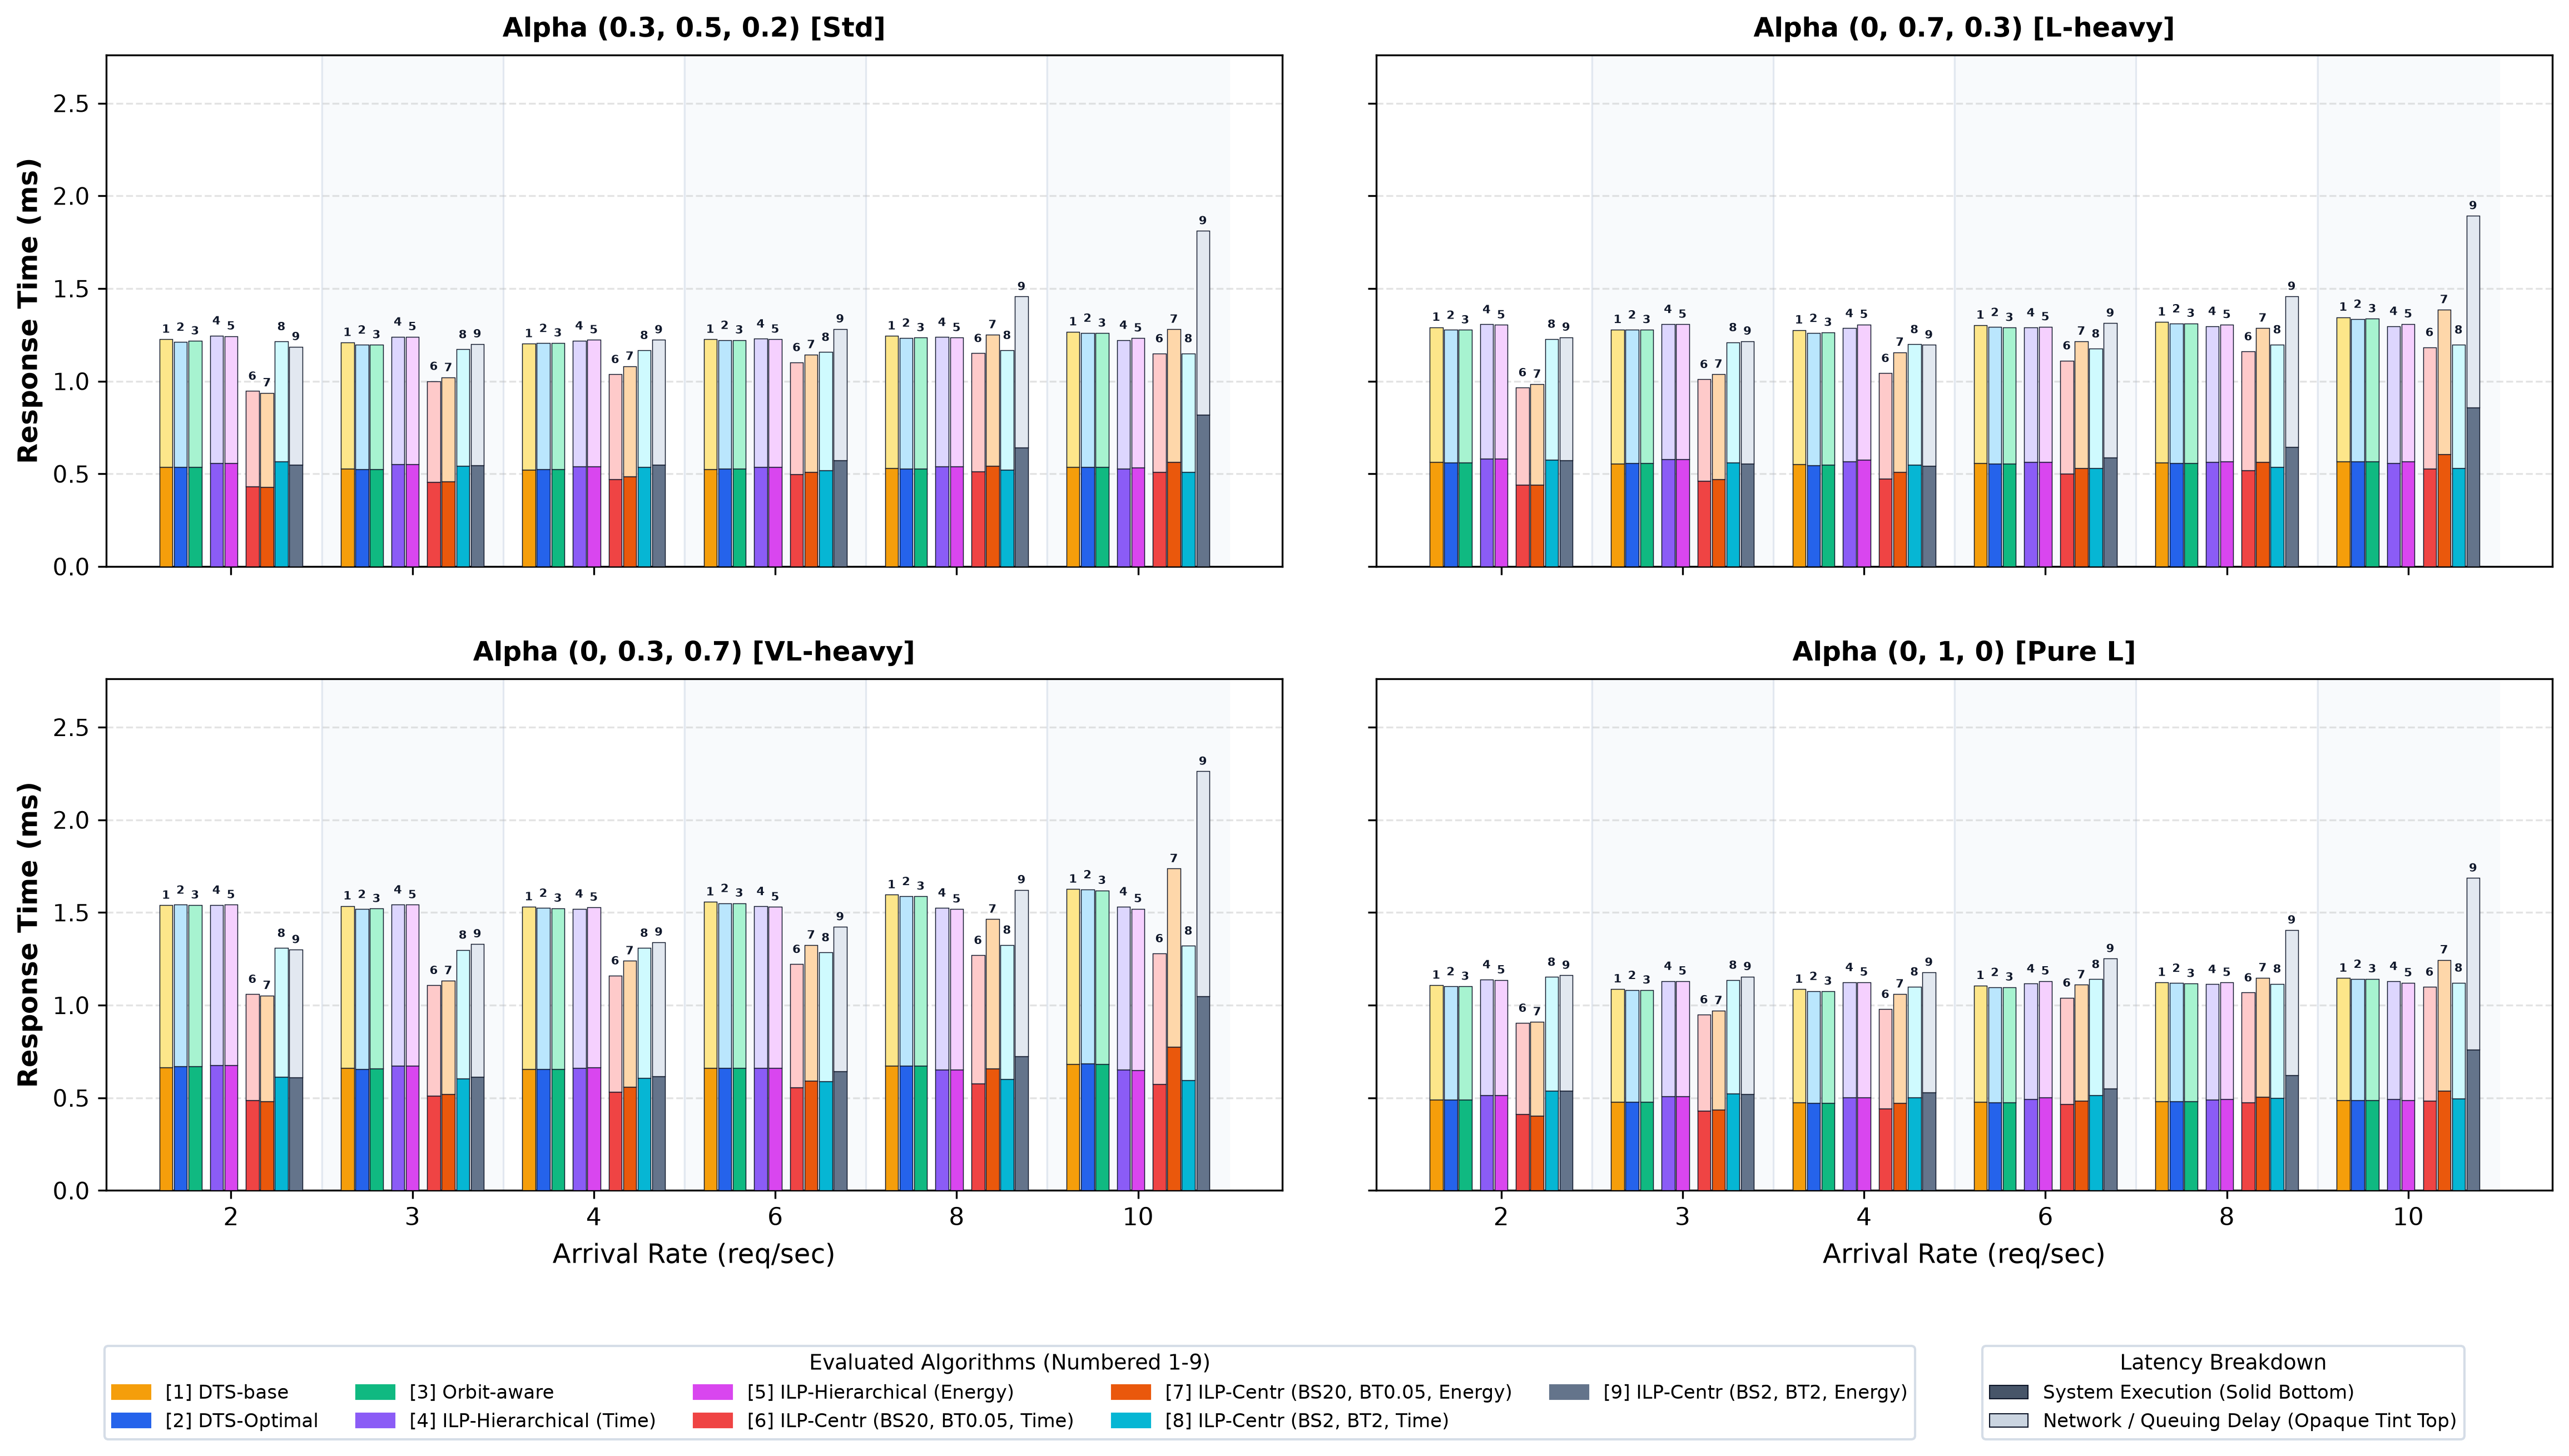
\includegraphics[width=\linewidth]{figures/02_Response_Time_Beta_0_0_1_80kJ.png}
        \caption{Response Time decomposition under Data-Intensive Workload $\boldsymbol{\beta} = (0, 0, 1)$ across arrival rates and battery capacities.}
        \label{fig:rt_data}
    \end{adjustwidth}
\end{figure}

\begin{figure}[H]
    \begin{adjustwidth}{-1.5cm}{-1.5cm}
        \centering
        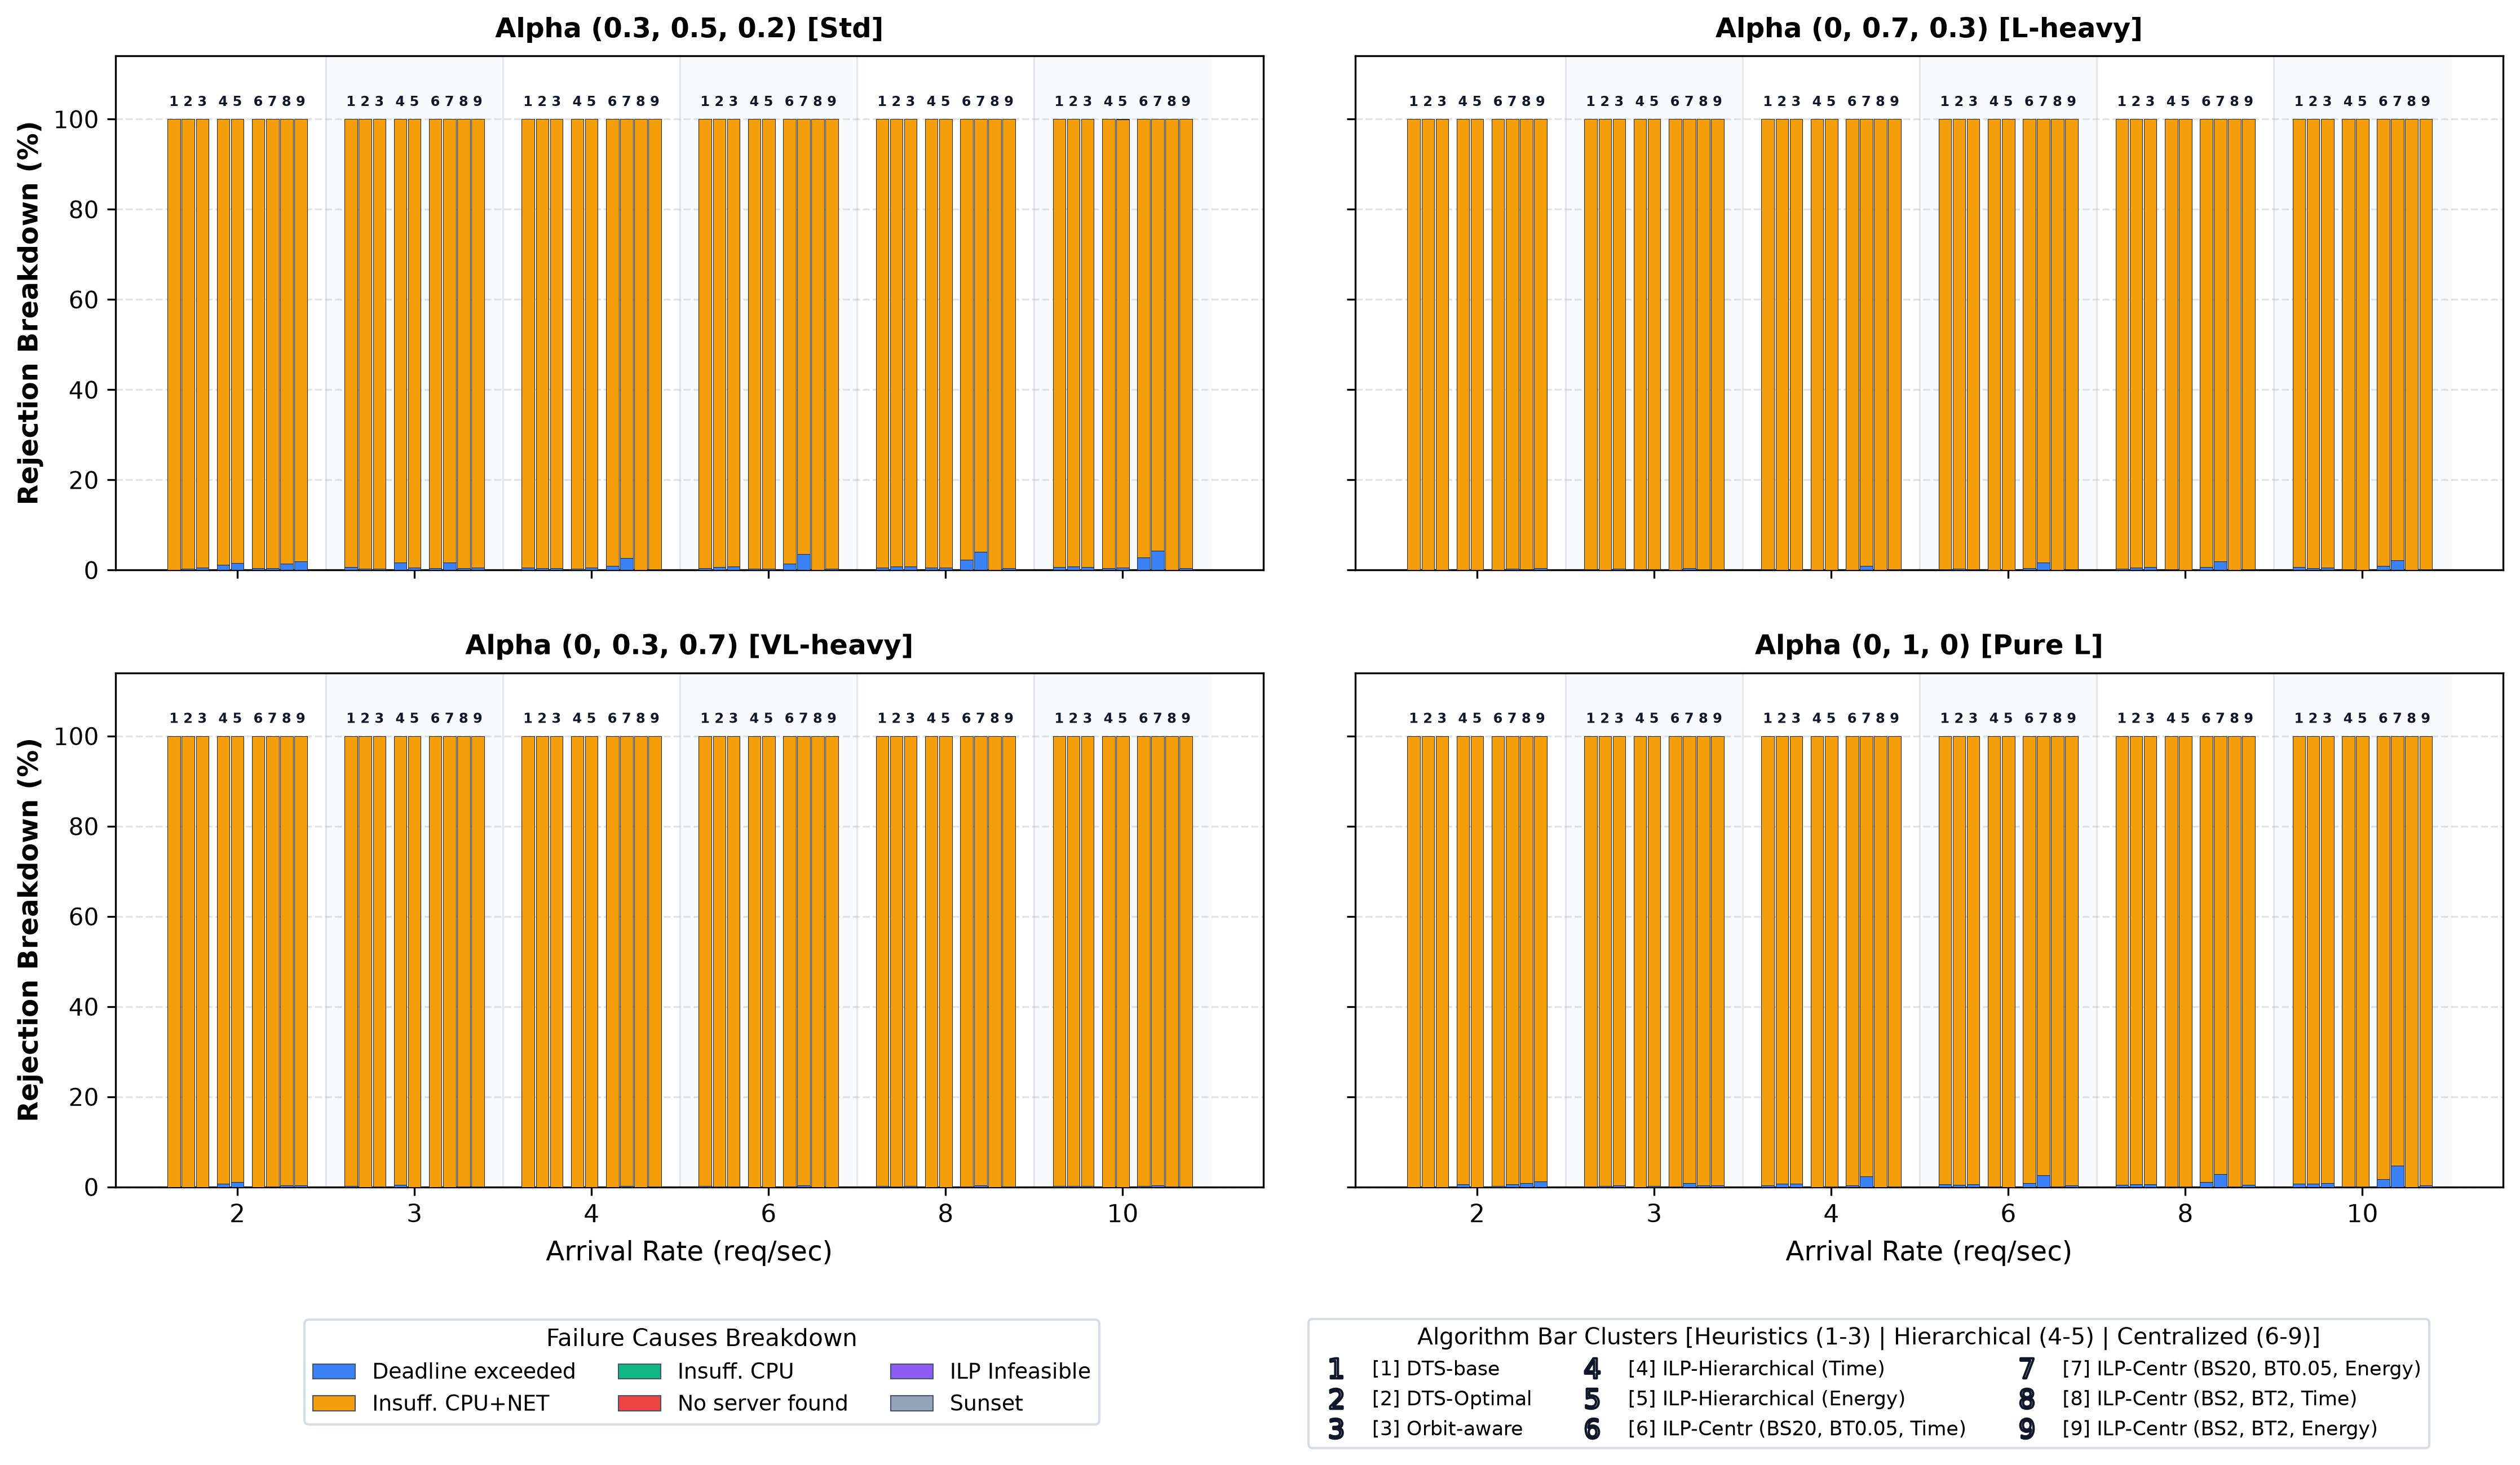
\includegraphics[width=\linewidth]{figures/03_Rejection_Causes_Beta_0_0_1_40kJ.png} \\
        \vspace{0.3cm}
        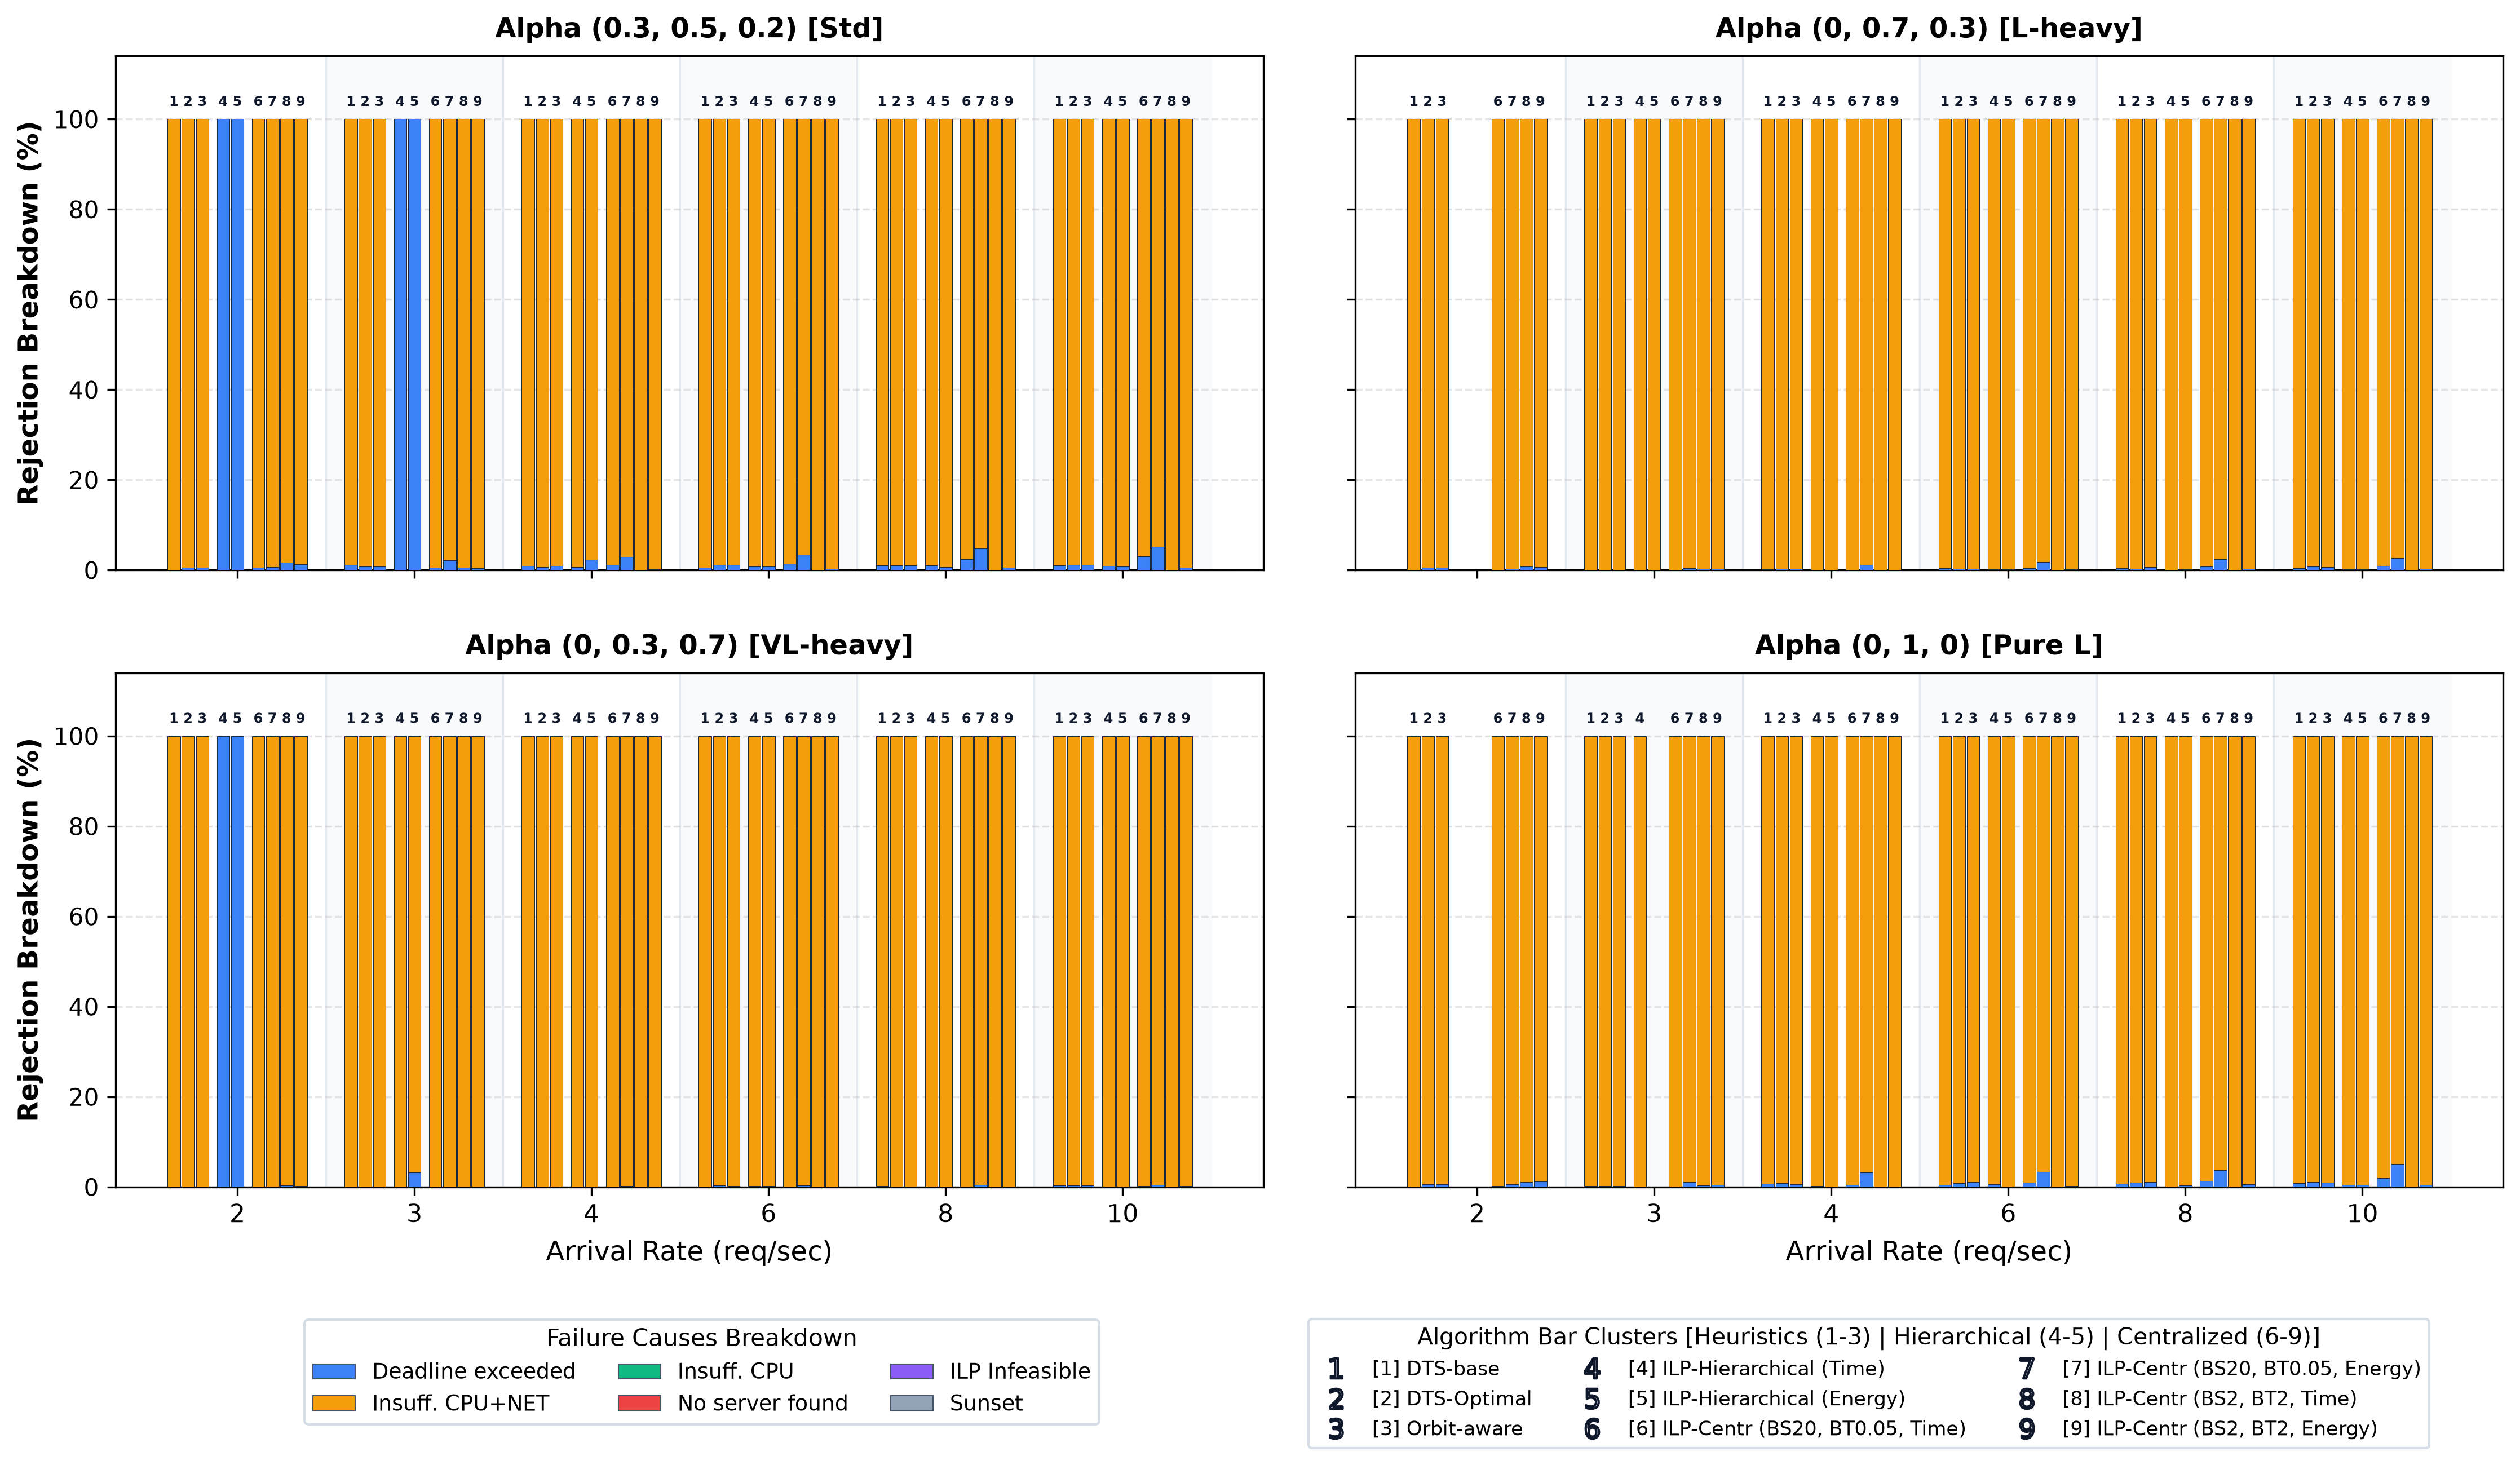
\includegraphics[width=\linewidth]{figures/03_Rejection_Causes_Beta_0_0_1_80kJ.png}
        \caption{Rejection Causes distribution under Data-Intensive Workload $\boldsymbol{\beta} = (0, 0, 1)$, showing the absolute dominance of joint link and energy saturation (\textit{Insuff. CPU+NET}).}
        \label{fig:rej_data}
    \end{adjustwidth}
\end{figure}

\subsubsection{Energy Elasticity and Global Optimality Supremacy}
The data-intensive scenario produces a remarkable inversion in algorithmic ranking. Transporting large payloads across optical links incurs heavy transceiver power consumption. At a tight $40\text{ kJ}$ budget, satellites exhaust their energy rapidly. However, doubling the capacity to $80\text{ kJ}$ unlocks massive throughput gains. Under $80\text{ kJ}$, mathematical optimization models decisively outperform distributed heuristics. \texttt{ILP-Hierarchical} achieves a near-perfect Success Rate of \textbf{$98\text{--}100\%$} at low loads. Furthermore, examining the $\boldsymbol{\alpha}$ sub-plots reveals that pushing payloads towards \textit{VL-heavy} or \textit{Pure L} drastically reduces heuristic efficiency, as their greedy, myopic routing logic saturates adjacent links, whereas ILP models successfully maneuver massive payloads around congested inter-plane routes.

\subsubsection{Structural Uniformity of Rejection Causes}
Figure~\ref{fig:rej_data} displays striking uniformity across all 9 algorithms: \textbf{virtually $100\%$ of all task rejections are categorized as \textit{Insufficient CPU+NET}} (orange bars). Rejections occur entirely because the joint requirement of massive data forwarding exhausts link transceivers and onboard battery budgets. The absolute absence of \textit{Deadline Exceeded} drops in this regime confirms that when local task computation is not the bottleneck, the physical infrastructure of the constellation dictates operational limits.

% =============================================================================
% SECTION 5.3: TRADE-OFF ANALYSIS AND OPERATIONAL GUIDELINES
% =============================================================================
\section{Trade-Off Analysis and Operational Discussion}
\label{sec:bench_tradeoffs}

Correlating the empirical findings across the 9 evaluated scenarios synthesizes four foundational operational trade-offs governing satellite task offloading.

\subsection{Theoretical Global Optimality vs. Ingress Queuing Latency}
\label{subsec:tradeoff_optimality_queuing}

The central dilemma of centralized satellite orchestration lies in the trade-off between global scheduling efficiency and ingress queuing latency:
\begin{itemize}
    \item \textbf{Distributed Heuristics:} Operate on an $M/M/1$ or $M/G/1$ queue with zero buffer aggregation. This responsiveness yields exceptional resilience against heavy request arrival rates preventing deadline expiration. However, lacking global visibility, heuristics make greedy, localized decisions that cause uneven battery drain and cannot avoid downstream link congestion (evidenced in the data-heavy scenarios).
    \item \textbf{Centralized ILP:} Solves an exact combinatorial problem over the entire constellation graph. While the actual execution time of the task on the target SEN remains bounded ($T_{exec} \le 0.30\text{ ms}$), the necessity of buffering requests to form optimization batches introduces static ingress delay ($T_{wait}$). In CPU-intensive scenarios, this waiting time consumes valuable deadline slack, triggering cascade rejections before tasks reach their assigned execution nodes.
\end{itemize}

\subsection{Energy Budget Sensitivity Across Dimensional Boundaries}
\label{subsec:tradeoff_energy_sensitivity}

Our results formally prove that battery reserve sizing ($40\text{ kJ}$ vs. $80\text{ kJ}$) exerts a heavily asymmetric impact depending on workload dimensionality:
\begin{itemize}
    \item \textbf{Compute-Bound Regimes ($\boldsymbol{\beta}=(0, 1, 0)$):} Highly inelastic to energy scaling. Adding battery reserves does not prevent processor queue overflow, and throughput curves remain static.
    \item \textbf{Communication-Bound Regimes ($\boldsymbol{\beta}=(0, 0, 1)$):} Highly elastic to energy scaling. Expanding battery capacity from $40\text{ kJ}$ to $80\text{ kJ}$ unlocks substantial throughput gains, enabling sustained multi-hop routing for heavy payloads without triggering early energy depletion.
\end{itemize}

\subsection{Architectural Synthesis and Deployment Guidelines}
\label{subsec:deployment_guidelines}

Based on the empirical evidence, Table~\ref{tab:synthesis_matrix} outlines prescriptive architectural guidelines recommending the optimal scheduling strategy based on mission profile and traffic conditions.

\begin{table}[ht!]
\centering
\small
\caption{Prescriptive architectural deployment matrix for Orbital Edge Computing missions.}
\label{tab:synthesis_matrix}
\begin{tabular}{@{}llll@{}}
\toprule
\textbf{Workload Characteristics} & \textbf{Traffic Regime} & \textbf{Recommended Paradigm} & \textbf{Primary Rationale} \\ \midrule
Data-Intensive (Large Payloads) & Low to Moderate & \texttt{ILP-Hierarchical / Centr} & Maximizes joint compute-routing efficiency \\
Data-Intensive (Large Payloads) & Heavy Stress & \texttt{DTS-Optimal} + Large Battery & Avoids ingress queuing collapse \\
CPU-Intensive (AI Inference) & Any Traffic & \texttt{OrbitAware / DTS-base} & Zero queuing; immediate drop on full CPU \\
Mixed Heterogeneous Services & $\lambda \le 4\text{ req/s}$ & \texttt{ILP-Centr (BS2, BT2)} & Balances joint allocation and energy \\
Mixed Heterogeneous Services & $\lambda > 6\text{ req/s}$ & \texttt{ILP-Centr (BS20, BT0.05)} & Low buffer dwell time; bounded latency \\ \bottomrule
\end{tabular}
\end{table}

% =============================================================================
% SECTION 5.4: SUMMARY OF CHAPTER FINDINGS
% =============================================================================
\section{Summary of Chapter Findings}
\label{sec:bench_summary}

The comprehensive comparative benchmark establishes four definitive conclusions:

\begin{enumerate}
    \item \textbf{Isolation of the Temporal vs. Physical Bottleneck:} In compute-heavy regimes, optimization-based failures are overwhelmingly driven by temporal deadline expiration (up to $90\%$ \textit{Deadline Exceeded}), whereas heuristic failures stem strictly from physical hardware limits ($100\%$ \textit{Insufficient CPU}).
    \item \textbf{Energy Elasticity in Data-Intensive Workloads:} Communication-heavy tasks reward global mathematical routing. ILP formulations achieve near-perfect success rates when supported by sufficient battery reserves ($80\text{ kJ}$), efficiently steering large payloads to avoid inter-plane link saturation.
    \item \textbf{Invariance of Local Node Execution ($T_{exec}$):} Across all scenarios, the physical task execution time on the assigned destination SEN remains strictly bounded ($<0.30\text{ ms}$), proving that performance degradation in centralized frameworks is caused by ingress batching latency, not localized computation logic or hardware limitations.
    \item \textbf{Absolute Elimination of Sunset Drops:} Across all 9 evaluated configurations and varying payload stresses, connection drops due to orbital eclipse remained consistently at $0\%$, confirming the absolute efficacy of the multi-objective sunset penalty $\gamma^*$.
\end{enumerate}

These empirical findings rigorously define the operational boundaries of centralized orbital orchestration, providing the foundation for the concluding assessments and future research directions presented in Chapter~\ref{chap:conclusions}.